\documentclass[twoside]{book}

% Packages required by doxygen
\usepackage{fixltx2e}
\usepackage{calc}
\usepackage{doxygen}
\usepackage[export]{adjustbox} % also loads graphicx
\usepackage{graphicx}
\usepackage[utf8]{inputenc}
\usepackage{makeidx}
\usepackage{multicol}
\usepackage{multirow}
\PassOptionsToPackage{warn}{textcomp}
\usepackage{textcomp}
\usepackage[nointegrals]{wasysym}
\usepackage[table]{xcolor}

% NLS support packages
\usepackage{hfont}

% Font selection
\usepackage[T1]{fontenc}
\usepackage[scaled=.90]{helvet}
\usepackage{courier}
\usepackage{amssymb}
\usepackage{sectsty}
\renewcommand{\familydefault}{\sfdefault}
\allsectionsfont{%
  \fontseries{bc}\selectfont%
  \color{darkgray}%
}
\renewcommand{\DoxyLabelFont}{%
  \fontseries{bc}\selectfont%
  \color{darkgray}%
}
\newcommand{\+}{\discretionary{\mbox{\scriptsize$\hookleftarrow$}}{}{}}

% Page & text layout
\usepackage{geometry}
\geometry{%
  a4paper,%
  top=2.5cm,%
  bottom=2.5cm,%
  left=2.5cm,%
  right=2.5cm%
}
\tolerance=750
\hfuzz=15pt
\hbadness=750
\setlength{\emergencystretch}{15pt}
\setlength{\parindent}{0cm}
\setlength{\parskip}{3ex plus 2ex minus 2ex}
\makeatletter
\renewcommand{\paragraph}{%
  \@startsection{paragraph}{4}{0ex}{-1.0ex}{1.0ex}{%
    \normalfont\normalsize\bfseries\SS@parafont%
  }%
}
\renewcommand{\subparagraph}{%
  \@startsection{subparagraph}{5}{0ex}{-1.0ex}{1.0ex}{%
    \normalfont\normalsize\bfseries\SS@subparafont%
  }%
}
\makeatother

% Headers & footers
\usepackage{fancyhdr}
\pagestyle{fancyplain}
\fancyhead[LE]{\fancyplain{}{\bfseries\thepage}}
\fancyhead[CE]{\fancyplain{}{}}
\fancyhead[RE]{\fancyplain{}{\bfseries\leftmark}}
\fancyhead[LO]{\fancyplain{}{\bfseries\rightmark}}
\fancyhead[CO]{\fancyplain{}{}}
\fancyhead[RO]{\fancyplain{}{\bfseries\thepage}}
\fancyfoot[LE]{\fancyplain{}{}}
\fancyfoot[CE]{\fancyplain{}{}}
\fancyfoot[RE]{\fancyplain{}{\bfseries\scriptsize 다음에 의해 생성됨 \+:  Doxygen }}
\fancyfoot[LO]{\fancyplain{}{\bfseries\scriptsize 다음에 의해 생성됨 \+:  Doxygen }}
\fancyfoot[CO]{\fancyplain{}{}}
\fancyfoot[RO]{\fancyplain{}{}}
\renewcommand{\footrulewidth}{0.4pt}
\renewcommand{\chaptermark}[1]{%
  \markboth{#1}{}%
}
\renewcommand{\sectionmark}[1]{%
  \markright{\thesection\ #1}%
}

% Indices & bibliography
\usepackage{natbib}
\usepackage[titles]{tocloft}
\setcounter{tocdepth}{3}
\setcounter{secnumdepth}{5}
\makeindex

% Hyperlinks (required, but should be loaded last)
\usepackage{ifpdf}
\ifpdf
  \usepackage[pdftex,pagebackref=true]{hyperref}
\else
  \usepackage[ps2pdf,pagebackref=true]{hyperref}
\fi
\hypersetup{%
  colorlinks=true,%
  linkcolor=blue,%
  citecolor=blue,%
  unicode%
}

% Custom commands
\newcommand{\clearemptydoublepage}{%
  \newpage{\pagestyle{empty}\cleardoublepage}%
}

\usepackage{caption}
\captionsetup{labelsep=space,justification=centering,font={bf},singlelinecheck=off,skip=4pt,position=top}

%===== C O N T E N T S =====

\begin{document}

% Titlepage & ToC
\hypersetup{pageanchor=false,
             bookmarksnumbered=true,
             pdfencoding=unicode
            }
\pagenumbering{roman}
\begin{titlepage}
\vspace*{7cm}
\begin{center}%
{\Large Keti\+WS }\\
\vspace*{1cm}
{\large 다음에 의해 생성됨 \+:  Doxygen 1.8.11}\\
\end{center}
\end{titlepage}
\clearemptydoublepage
\tableofcontents
\clearemptydoublepage
\pagenumbering{arabic}
\hypersetup{pageanchor=true}

%--- Begin generated contents ---
\chapter{Keti Local Planning Package}
\label{index}\hypertarget{index}{}\hypertarget{index_Introduction}{}\section{Introduction}\label{index_Introduction}
This package generates local path 
\chapter{모듈 색인}
\section{모듈}
다음은 모든 모듈들의 목록입니다.\+:\begin{DoxyCompactList}
\item \contentsline{section}{main}{\pageref{group___main_group}}{}
\item \contentsline{section}{algorithm}{\pageref{group___algorithm_group}}{}
\item \contentsline{section}{data}{\pageref{group___data_group}}{}
\item \contentsline{section}{data handling}{\pageref{group___data_handling_group}}{}
\end{DoxyCompactList}

\chapter{클래스 색인}
\section{클래스 목록}
다음은 클래스, 구조체, 공용체 그리고 인터페이스들입니다. (간략한 설명만을 보여줍니다) \+:\begin{DoxyCompactList}
\item\contentsline{section}{\hyperlink{class_angle_utils}{Angle\+Utils} }{\pageref{class_angle_utils}}{}
\item\contentsline{section}{\hyperlink{class_c_keti_local_planning}{C\+Keti\+Local\+Planning} \\*Planning local path avoiding obstacle and following lane }{\pageref{class_c_keti_local_planning}}{}
\item\contentsline{section}{\hyperlink{class_g_p_s_point}{G\+P\+S\+Point} \\*Type representing class containing (x,y,z,a) }{\pageref{class_g_p_s_point}}{}
\item\contentsline{section}{\hyperlink{class_lane_array_handler}{Lane\+Array\+Handler} \\*The Type\+Conversion class This class is handling lane array information }{\pageref{class_lane_array_handler}}{}
\item\contentsline{section}{\hyperlink{class_lane_handler}{Lane\+Handler} \\*This class treats lane information with autowar\+\_\+msgs\+::lane and std\+::vector$<$\+Way\+Point$>$ }{\pageref{class_lane_handler}}{}
\item\contentsline{section}{\hyperlink{class_point_handler}{Point\+Handler} \\*Point handling class }{\pageref{class_point_handler}}{}
\item\contentsline{section}{\hyperlink{class_pose_point_handler}{Pose\+Point\+Handler} \\*The Pose\+Position\+Handler class }{\pageref{class_pose_point_handler}}{}
\item\contentsline{section}{\hyperlink{class_ros_helpers}{Ros\+Helpers} }{\pageref{class_ros_helpers}}{}
\item\contentsline{section}{\hyperlink{class_way_point}{Way\+Point} \\*Type representing class containing (\hyperlink{class_g_p_s_point}{G\+P\+S\+Point}, v) }{\pageref{class_way_point}}{}
\end{DoxyCompactList}

\chapter{파일 색인}
\section{파일 목록}
다음은 모든 파일에 대한 목록입니다. (간략한 설명만을 보여줍니다) \+:\begin{DoxyCompactList}
\item\contentsline{section}{/home/dallddungi/keti\+\_\+ws/src/keti\+\_\+local\+\_\+planning/include/\hyperlink{cketilocalplanning_8h}{cketilocalplanning.\+h} }{\pageref{cketilocalplanning_8h}}{}
\item\contentsline{section}{/home/dallddungi/keti\+\_\+ws/src/keti\+\_\+local\+\_\+planning/include/\hyperlink{projectinfo_8h}{projectinfo.\+h} }{\pageref{projectinfo_8h}}{}
\item\contentsline{section}{/home/dallddungi/keti\+\_\+ws/src/keti\+\_\+local\+\_\+planning/include/\hyperlink{ros__helpers_8h}{ros\+\_\+helpers.\+h} }{\pageref{ros__helpers_8h}}{}
\item\contentsline{section}{/home/dallddungi/keti\+\_\+ws/src/keti\+\_\+local\+\_\+planning/include/data\+\_\+classes/\hyperlink{gpspoint_8h}{gpspoint.\+h} }{\pageref{gpspoint_8h}}{}
\item\contentsline{section}{/home/dallddungi/keti\+\_\+ws/src/keti\+\_\+local\+\_\+planning/include/data\+\_\+classes/\hyperlink{waypoint_8h}{waypoint.\+h} }{\pageref{waypoint_8h}}{}
\item\contentsline{section}{/home/dallddungi/keti\+\_\+ws/src/keti\+\_\+local\+\_\+planning/include/data\+\_\+handler/\hyperlink{lane__handler_8h}{lane\+\_\+handler.\+h} }{\pageref{lane__handler_8h}}{}
\item\contentsline{section}{/home/dallddungi/keti\+\_\+ws/src/keti\+\_\+local\+\_\+planning/include/data\+\_\+handler/\hyperlink{lanearray__handler_8h}{lanearray\+\_\+handler.\+h} }{\pageref{lanearray__handler_8h}}{}
\item\contentsline{section}{/home/dallddungi/keti\+\_\+ws/src/keti\+\_\+local\+\_\+planning/include/data\+\_\+handler/\hyperlink{point__handler_8h}{point\+\_\+handler.\+h} }{\pageref{point__handler_8h}}{}
\item\contentsline{section}{/home/dallddungi/keti\+\_\+ws/src/keti\+\_\+local\+\_\+planning/include/data\+\_\+handler/\hyperlink{pose__point__handler_8h}{pose\+\_\+point\+\_\+handler.\+h} }{\pageref{pose__point__handler_8h}}{}
\item\contentsline{section}{/home/dallddungi/keti\+\_\+ws/src/keti\+\_\+local\+\_\+planning/include/utils/\hyperlink{angle__utils_8h}{angle\+\_\+utils.\+h} }{\pageref{angle__utils_8h}}{}
\item\contentsline{section}{/home/dallddungi/keti\+\_\+ws/src/keti\+\_\+local\+\_\+planning/include/utils/\hyperlink{math__constant_8h}{math\+\_\+constant.\+h} }{\pageref{math__constant_8h}}{}
\item\contentsline{section}{/home/dallddungi/keti\+\_\+ws/src/keti\+\_\+local\+\_\+planning/src/\hyperlink{cketilocalplanning_8cpp}{cketilocalplanning.\+cpp} }{\pageref{cketilocalplanning_8cpp}}{}
\item\contentsline{section}{/home/dallddungi/keti\+\_\+ws/src/keti\+\_\+local\+\_\+planning/src/\hyperlink{ketilocalplanning__main_8cpp}{ketilocalplanning\+\_\+main.\+cpp} }{\pageref{ketilocalplanning__main_8cpp}}{}
\item\contentsline{section}{/home/dallddungi/keti\+\_\+ws/src/keti\+\_\+local\+\_\+planning/src/\hyperlink{ros__helpers_8cpp}{ros\+\_\+helpers.\+cpp} }{\pageref{ros__helpers_8cpp}}{}
\item\contentsline{section}{/home/dallddungi/keti\+\_\+ws/src/keti\+\_\+local\+\_\+planning/src/data\+\_\+handler/\hyperlink{lane__handler_8cpp}{lane\+\_\+handler.\+cpp} }{\pageref{lane__handler_8cpp}}{}
\item\contentsline{section}{/home/dallddungi/keti\+\_\+ws/src/keti\+\_\+local\+\_\+planning/src/data\+\_\+handler/\hyperlink{lanearray__handler_8cpp}{lanearray\+\_\+handler.\+cpp} }{\pageref{lanearray__handler_8cpp}}{}
\item\contentsline{section}{/home/dallddungi/keti\+\_\+ws/src/keti\+\_\+local\+\_\+planning/src/data\+\_\+handler/\hyperlink{pose__point__handler_8cpp}{pose\+\_\+point\+\_\+handler.\+cpp} }{\pageref{pose__point__handler_8cpp}}{}
\item\contentsline{section}{/home/dallddungi/keti\+\_\+ws/src/keti\+\_\+local\+\_\+planning/src/utils/\hyperlink{angle__utils_8cpp}{angle\+\_\+utils.\+cpp} }{\pageref{angle__utils_8cpp}}{}
\end{DoxyCompactList}

\chapter{모듈 문서화}
\hypertarget{group___main_group}{}\section{main}
\label{group___main_group}\index{main@{main}}
\subsection*{클래스}
\begin{DoxyCompactItemize}
\item 
class \hyperlink{class_c_keti_local_planning}{C\+Keti\+Local\+Planning}
\begin{DoxyCompactList}\small\item\em Planning local path avoiding obstacle and following lane. \end{DoxyCompactList}\end{DoxyCompactItemize}


\subsection{상세한 설명}

\hypertarget{group___algorithm_group}{}\section{algorithm}
\label{group___algorithm_group}\index{algorithm@{algorithm}}
Algorithm related class of Local Planning Library 
\hypertarget{group___data_group}{}\section{data}
\label{group___data_group}\index{data@{data}}
\subsection*{클래스}
\begin{DoxyCompactItemize}
\item 
class \hyperlink{class_g_p_s_point}{G\+P\+S\+Point}
\begin{DoxyCompactList}\small\item\em type representing class containing (x,y,z,a) \end{DoxyCompactList}\item 
class \hyperlink{class_way_point}{Way\+Point}
\begin{DoxyCompactList}\small\item\em type representing class containing (\hyperlink{class_g_p_s_point}{G\+P\+S\+Point}, v) \end{DoxyCompactList}\end{DoxyCompactItemize}


\subsection{상세한 설명}
Data related class of Local Planning Library 
\hypertarget{group___data_handling_group}{}\section{data handling}
\label{group___data_handling_group}\index{data handling@{data handling}}
\subsection*{클래스}
\begin{DoxyCompactItemize}
\item 
class \hyperlink{class_lane_handler}{Lane\+Handler}
\begin{DoxyCompactList}\small\item\em This class treats lane information with autowar\+\_\+msgs\+::lane and std\+::vector$<$\+Way\+Point$>$ \end{DoxyCompactList}\item 
class \hyperlink{class_lane_array_handler}{Lane\+Array\+Handler}
\begin{DoxyCompactList}\small\item\em The Type\+Conversion class This class is handling lane array information. \end{DoxyCompactList}\item 
class \hyperlink{class_point_handler}{Point\+Handler}
\begin{DoxyCompactList}\small\item\em Point handling class. \end{DoxyCompactList}\item 
class \hyperlink{class_pose_point_handler}{Pose\+Point\+Handler}
\begin{DoxyCompactList}\small\item\em The Pose\+Position\+Handler class. \end{DoxyCompactList}\end{DoxyCompactItemize}


\subsection{상세한 설명}

\chapter{클래스 문서화}
\hypertarget{class_angle_utils}{}\section{Angle\+Utils 클래스 참조}
\label{class_angle_utils}\index{Angle\+Utils@{Angle\+Utils}}


{\ttfamily \#include $<$angle\+\_\+utils.\+h$>$}



Angle\+Utils에 대한 협력 다이어그램\+:\nopagebreak
\begin{figure}[H]
\begin{center}
\leavevmode
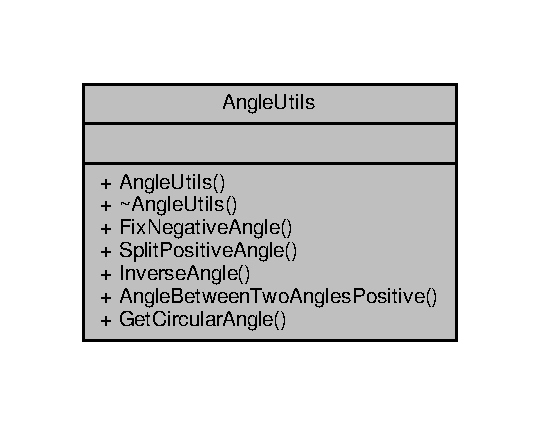
\includegraphics[width=259pt]{class_angle_utils__coll__graph}
\end{center}
\end{figure}
\subsection*{Public 멤버 함수}
\begin{DoxyCompactItemize}
\item 
\hyperlink{class_angle_utils_a244b7e39d429d0667180ee1f6c4688dc}{Angle\+Utils} ()
\item 
virtual \hyperlink{class_angle_utils_afd7d97d10e25e67dfad8a3700168f796}{$\sim$\+Angle\+Utils} ()
\end{DoxyCompactItemize}
\subsection*{정적 Public 멤버 함수}
\begin{DoxyCompactItemize}
\item 
static double \hyperlink{class_angle_utils_a27d9bd3a5b5816f9b94dbdadc785a75d}{Fix\+Negative\+Angle} (const double \&a)
\item 
static double \hyperlink{class_angle_utils_a91f3e34c9e1e35788d44a2f6bc5bc206}{Split\+Positive\+Angle} (const double \&a)
\item 
static double \hyperlink{class_angle_utils_a90a3b153450f72621fa4d601630f7999}{Inverse\+Angle} (const double \&a)
\item 
static double \hyperlink{class_angle_utils_aa9a3fb876a9b6d446a8033d2f901bb73}{Angle\+Between\+Two\+Angles\+Positive} (const double \&a1, const double \&a2)
\item 
static double \hyperlink{class_angle_utils_a5a51b312ed27e10ab9af2e092a897da7}{Get\+Circular\+Angle} (const double \&prev\+Cont\+Angle, const double \&prev\+Angle, const double \&curr\+Angle)
\end{DoxyCompactItemize}


\subsection{상세한 설명}


angle\+\_\+utils.\+h 파일의 8 번째 라인에서 정의되었습니다.



\subsection{생성자 \& 소멸자 문서화}
\index{Angle\+Utils@{Angle\+Utils}!Angle\+Utils@{Angle\+Utils}}
\index{Angle\+Utils@{Angle\+Utils}!Angle\+Utils@{Angle\+Utils}}
\subsubsection[{\texorpdfstring{Angle\+Utils()}{AngleUtils()}}]{\setlength{\rightskip}{0pt plus 5cm}Angle\+Utils\+::\+Angle\+Utils (
\begin{DoxyParamCaption}
{}
\end{DoxyParamCaption}
)}\hypertarget{class_angle_utils_a244b7e39d429d0667180ee1f6c4688dc}{}\label{class_angle_utils_a244b7e39d429d0667180ee1f6c4688dc}


angle\+\_\+utils.\+cpp 파일의 3 번째 라인에서 정의되었습니다.


\begin{DoxyCode}
4 \{
5 \}
\end{DoxyCode}
\index{Angle\+Utils@{Angle\+Utils}!````~Angle\+Utils@{$\sim$\+Angle\+Utils}}
\index{````~Angle\+Utils@{$\sim$\+Angle\+Utils}!Angle\+Utils@{Angle\+Utils}}
\subsubsection[{\texorpdfstring{$\sim$\+Angle\+Utils()}{~AngleUtils()}}]{\setlength{\rightskip}{0pt plus 5cm}Angle\+Utils\+::$\sim$\+Angle\+Utils (
\begin{DoxyParamCaption}
{}
\end{DoxyParamCaption}
)\hspace{0.3cm}{\ttfamily [virtual]}}\hypertarget{class_angle_utils_afd7d97d10e25e67dfad8a3700168f796}{}\label{class_angle_utils_afd7d97d10e25e67dfad8a3700168f796}


angle\+\_\+utils.\+cpp 파일의 7 번째 라인에서 정의되었습니다.


\begin{DoxyCode}
8 \{
9 \}
\end{DoxyCode}


\subsection{멤버 함수 문서화}
\index{Angle\+Utils@{Angle\+Utils}!Angle\+Between\+Two\+Angles\+Positive@{Angle\+Between\+Two\+Angles\+Positive}}
\index{Angle\+Between\+Two\+Angles\+Positive@{Angle\+Between\+Two\+Angles\+Positive}!Angle\+Utils@{Angle\+Utils}}
\subsubsection[{\texorpdfstring{Angle\+Between\+Two\+Angles\+Positive(const double \&a1, const double \&a2)}{AngleBetweenTwoAnglesPositive(const double &a1, const double &a2)}}]{\setlength{\rightskip}{0pt plus 5cm}double Angle\+Utils\+::\+Angle\+Between\+Two\+Angles\+Positive (
\begin{DoxyParamCaption}
\item[{const double \&}]{a1, }
\item[{const double \&}]{a2}
\end{DoxyParamCaption}
)\hspace{0.3cm}{\ttfamily [static]}}\hypertarget{class_angle_utils_aa9a3fb876a9b6d446a8033d2f901bb73}{}\label{class_angle_utils_aa9a3fb876a9b6d446a8033d2f901bb73}


angle\+\_\+utils.\+cpp 파일의 65 번째 라인에서 정의되었습니다.


\begin{DoxyCode}
66 \{
67    \textcolor{keywordtype}{double} diff = a1 - a2;
68    \textcolor{keywordflow}{if}(diff < 0)
69      diff = a2 - a1;
70 
71    \textcolor{keywordflow}{if}(diff > M\_PI)
72      diff = 2.0*M\_PI - diff;
73 
74    \textcolor{keywordflow}{return} diff;
75 \}
\end{DoxyCode}
\index{Angle\+Utils@{Angle\+Utils}!Fix\+Negative\+Angle@{Fix\+Negative\+Angle}}
\index{Fix\+Negative\+Angle@{Fix\+Negative\+Angle}!Angle\+Utils@{Angle\+Utils}}
\subsubsection[{\texorpdfstring{Fix\+Negative\+Angle(const double \&a)}{FixNegativeAngle(const double &a)}}]{\setlength{\rightskip}{0pt plus 5cm}double Angle\+Utils\+::\+Fix\+Negative\+Angle (
\begin{DoxyParamCaption}
\item[{const double \&}]{a}
\end{DoxyParamCaption}
)\hspace{0.3cm}{\ttfamily [static]}}\hypertarget{class_angle_utils_a27d9bd3a5b5816f9b94dbdadc785a75d}{}\label{class_angle_utils_a27d9bd3a5b5816f9b94dbdadc785a75d}


angle\+\_\+utils.\+cpp 파일의 13 번째 라인에서 정의되었습니다.


\begin{DoxyCode}
14 \{
15    \textcolor{keywordtype}{double} angle = 0;
16    \textcolor{keywordflow}{if} (a < -2.0*M\_PI || a > 2.0*M\_PI)
17   \{
18      angle = fmod(a, 2.0*M\_PI);
19   \}
20    \textcolor{keywordflow}{else}
21      angle = a;
22 
23 
24    \textcolor{keywordflow}{if}(angle < 0)
25    \{
26      angle = 2.0*M\_PI + angle;
27    \}
28 
29    \textcolor{keywordflow}{return} angle;
30 \}
\end{DoxyCode}
\index{Angle\+Utils@{Angle\+Utils}!Get\+Circular\+Angle@{Get\+Circular\+Angle}}
\index{Get\+Circular\+Angle@{Get\+Circular\+Angle}!Angle\+Utils@{Angle\+Utils}}
\subsubsection[{\texorpdfstring{Get\+Circular\+Angle(const double \&prev\+Cont\+Angle, const double \&prev\+Angle, const double \&curr\+Angle)}{GetCircularAngle(const double &prevContAngle, const double &prevAngle, const double &currAngle)}}]{\setlength{\rightskip}{0pt plus 5cm}double Angle\+Utils\+::\+Get\+Circular\+Angle (
\begin{DoxyParamCaption}
\item[{const double \&}]{prev\+Cont\+Angle, }
\item[{const double \&}]{prev\+Angle, }
\item[{const double \&}]{curr\+Angle}
\end{DoxyParamCaption}
)\hspace{0.3cm}{\ttfamily [static]}}\hypertarget{class_angle_utils_a5a51b312ed27e10ab9af2e092a897da7}{}\label{class_angle_utils_a5a51b312ed27e10ab9af2e092a897da7}


angle\+\_\+utils.\+cpp 파일의 77 번째 라인에서 정의되었습니다.


\begin{DoxyCode}
78 \{
79 
80   \textcolor{keywordtype}{double} diff = currAngle - prevAngle;
81   \textcolor{keywordflow}{if}(diff > M\_PI)
82     diff = diff - 2.0*M\_PI;
83   \textcolor{keywordflow}{if}(diff < -M\_PI)
84     diff = diff + 2.0*M\_PI;
85 
86   \textcolor{keywordtype}{double} c\_ang = 0;
87   \textcolor{keywordflow}{if}(prevContAngle == 0 || fabs(diff) < M\_PI\_2)
88      c\_ang = prevContAngle + diff;
89   \textcolor{keywordflow}{else}
90     c\_ang = prevContAngle;
91 
92   \textcolor{keywordflow}{return} c\_ang;
93 \}
\end{DoxyCode}
\index{Angle\+Utils@{Angle\+Utils}!Inverse\+Angle@{Inverse\+Angle}}
\index{Inverse\+Angle@{Inverse\+Angle}!Angle\+Utils@{Angle\+Utils}}
\subsubsection[{\texorpdfstring{Inverse\+Angle(const double \&a)}{InverseAngle(const double &a)}}]{\setlength{\rightskip}{0pt plus 5cm}double Angle\+Utils\+::\+Inverse\+Angle (
\begin{DoxyParamCaption}
\item[{const double \&}]{a}
\end{DoxyParamCaption}
)\hspace{0.3cm}{\ttfamily [static]}}\hypertarget{class_angle_utils_a90a3b153450f72621fa4d601630f7999}{}\label{class_angle_utils_a90a3b153450f72621fa4d601630f7999}


angle\+\_\+utils.\+cpp 파일의 53 번째 라인에서 정의되었습니다.


\begin{DoxyCode}
54 \{
55 
56    \textcolor{keywordtype}{double} angle = 0;
57    \textcolor{keywordflow}{if}(a <= M\_PI)
58     angle =  a + M\_PI;
59   \textcolor{keywordflow}{else}
60     angle = a - M\_PI;
61 
62    \textcolor{keywordflow}{return} angle;
63 \}
\end{DoxyCode}
\index{Angle\+Utils@{Angle\+Utils}!Split\+Positive\+Angle@{Split\+Positive\+Angle}}
\index{Split\+Positive\+Angle@{Split\+Positive\+Angle}!Angle\+Utils@{Angle\+Utils}}
\subsubsection[{\texorpdfstring{Split\+Positive\+Angle(const double \&a)}{SplitPositiveAngle(const double &a)}}]{\setlength{\rightskip}{0pt plus 5cm}double Angle\+Utils\+::\+Split\+Positive\+Angle (
\begin{DoxyParamCaption}
\item[{const double \&}]{a}
\end{DoxyParamCaption}
)\hspace{0.3cm}{\ttfamily [static]}}\hypertarget{class_angle_utils_a91f3e34c9e1e35788d44a2f6bc5bc206}{}\label{class_angle_utils_a91f3e34c9e1e35788d44a2f6bc5bc206}


angle\+\_\+utils.\+cpp 파일의 32 번째 라인에서 정의되었습니다.


\begin{DoxyCode}
33 \{
34    \textcolor{keywordtype}{double} angle = a;
35 
36   \textcolor{keywordflow}{if} (a < -2.0*M\_PI || a > 2.0*M\_PI)
37   \{
38     angle = fmod(a, 2.0*M\_PI);
39   \}
40 
41   \textcolor{keywordflow}{if} (angle > M\_PI)
42   \{
43     angle -= 2.0*M\_PI;
44   \}
45   \textcolor{keywordflow}{else} \textcolor{keywordflow}{if} (angle < -M\_PI)
46   \{
47     angle += 2.0*M\_PI;
48   \}
49 
50   \textcolor{keywordflow}{return} angle;
51 \}
\end{DoxyCode}


이 함수를 호출하는 함수들에 대한 그래프입니다.\+:\nopagebreak
\begin{figure}[H]
\begin{center}
\leavevmode
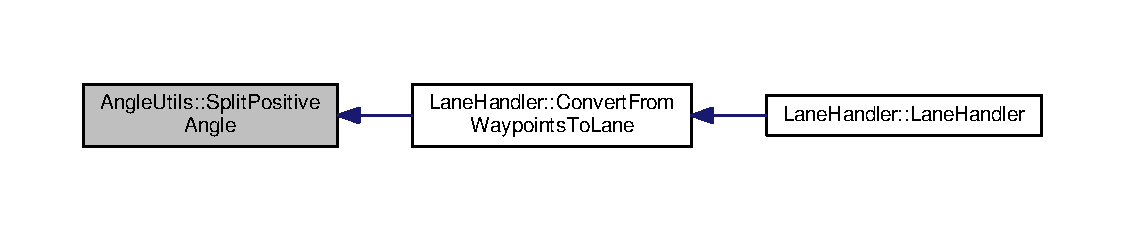
\includegraphics[width=350pt]{class_angle_utils_a91f3e34c9e1e35788d44a2f6bc5bc206_icgraph}
\end{center}
\end{figure}




이 클래스에 대한 문서화 페이지는 다음의 파일들로부터 생성되었습니다.\+:\begin{DoxyCompactItemize}
\item 
/home/dallddungi/keti\+\_\+ws/src/keti\+\_\+local\+\_\+planning/include/utils/\hyperlink{angle__utils_8h}{angle\+\_\+utils.\+h}\item 
/home/dallddungi/keti\+\_\+ws/src/keti\+\_\+local\+\_\+planning/src/utils/\hyperlink{angle__utils_8cpp}{angle\+\_\+utils.\+cpp}\end{DoxyCompactItemize}

\hypertarget{class_c_keti_local_planning}{}\section{C\+Keti\+Local\+Planning 클래스 참조}
\label{class_c_keti_local_planning}\index{C\+Keti\+Local\+Planning@{C\+Keti\+Local\+Planning}}


Planning local path avoiding obstacle and following lane.  




{\ttfamily \#include $<$cketilocalplanning.\+h$>$}



C\+Keti\+Local\+Planning에 대한 협력 다이어그램\+:\nopagebreak
\begin{figure}[H]
\begin{center}
\leavevmode
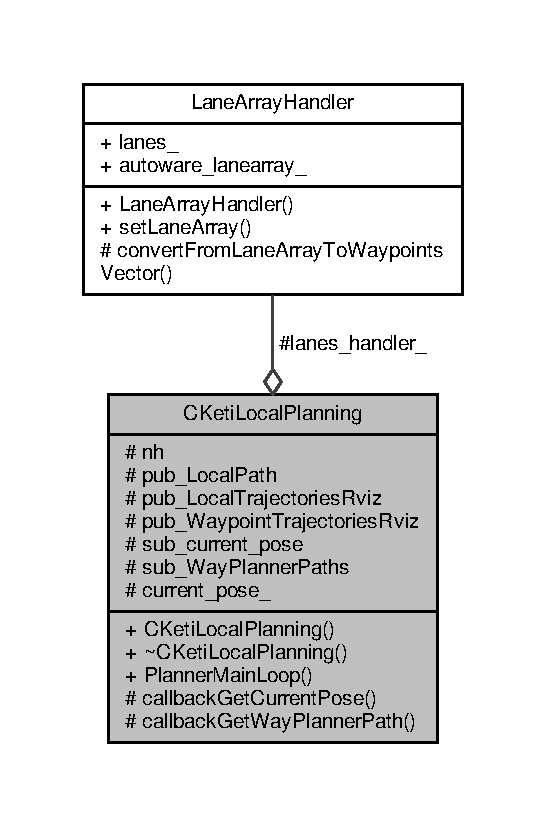
\includegraphics[width=262pt]{class_c_keti_local_planning__coll__graph}
\end{center}
\end{figure}
\subsection*{Public 멤버 함수}
\begin{DoxyCompactItemize}
\item 
\hyperlink{class_c_keti_local_planning_a64e789f070f7334aab7727c0ae276931}{C\+Keti\+Local\+Planning} ()
\item 
\hyperlink{class_c_keti_local_planning_adab5b7e3683328d05b50ed802e2fb5cd}{$\sim$\+C\+Keti\+Local\+Planning} ()
\item 
void \hyperlink{class_c_keti_local_planning_a3286318e734e7441036b43cec169978c}{Planner\+Main\+Loop} ()
\end{DoxyCompactItemize}
\subsection*{Protected 멤버 함수}
\begin{DoxyCompactItemize}
\item 
void \hyperlink{class_c_keti_local_planning_a144131de19f37584bab4412f98e1fc63}{callback\+Get\+Current\+Pose} (const geometry\+\_\+msgs\+::\+Pose\+Stamped\+Const\+Ptr \&msg)
\begin{DoxyCompactList}\small\item\em callback\+Get\+Current\+Pose \end{DoxyCompactList}\item 
void \hyperlink{class_c_keti_local_planning_ab385a1021d3d90f9f2b7b5a40dd791c2}{callback\+Get\+Way\+Planner\+Path} (const autoware\+\_\+msgs\+::\+Lane\+Array \&msg)
\begin{DoxyCompactList}\small\item\em callback\+Get\+Way\+Planner\+Path \end{DoxyCompactList}\end{DoxyCompactItemize}
\subsection*{Protected 속성}
\begin{DoxyCompactItemize}
\item 
ros\+::\+Node\+Handle \hyperlink{class_c_keti_local_planning_a39a260e89fa7805f6c0c7112c91cb847}{nh}
\item 
ros\+::\+Publisher \hyperlink{class_c_keti_local_planning_a42f394ae6069296e6f412eb5daa9dd3a}{pub\+\_\+\+Local\+Path}
\item 
ros\+::\+Publisher \hyperlink{class_c_keti_local_planning_a423ed1137dde91f12793bdcacb4e0bea}{pub\+\_\+\+Local\+Trajectories\+Rviz}
\item 
ros\+::\+Publisher \hyperlink{class_c_keti_local_planning_a54aec2f11f157100a74b09a9cf5fa38b}{pub\+\_\+\+Waypoint\+Trajectories\+Rviz}
\item 
ros\+::\+Subscriber \hyperlink{class_c_keti_local_planning_ac399c600a59f7b79448ba1f1bbfda8ca}{sub\+\_\+current\+\_\+pose}
\item 
ros\+::\+Subscriber \hyperlink{class_c_keti_local_planning_a75e59488889af86a89995f2c606677ce}{sub\+\_\+\+Way\+Planner\+Paths}
\item 
geometry\+\_\+msgs\+::\+Pose \hyperlink{class_c_keti_local_planning_a4f4dcb94c250fb4d324b33f2fa42ffcb}{current\+\_\+pose\+\_\+}
\item 
\hyperlink{class_lane_array_handler}{Lane\+Array\+Handler} \hyperlink{class_c_keti_local_planning_a6295120665288244397783d747cc60cf}{lanes\+\_\+handler\+\_\+}
\end{DoxyCompactItemize}


\subsection{상세한 설명}
Planning local path avoiding obstacle and following lane. 

\begin{DoxyAuthor}{작성자}
Yunjeong Kim(\href{mailto:dallddungi@naver.com}{\tt dallddungi@naver.\+com})
\end{DoxyAuthor}
It generates local path consisting of waypoints which follwoing lane while avoiding obstacles. 

cketilocalplanning.\+h 파일의 19 번째 라인에서 정의되었습니다.



\subsection{생성자 \& 소멸자 문서화}
\index{C\+Keti\+Local\+Planning@{C\+Keti\+Local\+Planning}!C\+Keti\+Local\+Planning@{C\+Keti\+Local\+Planning}}
\index{C\+Keti\+Local\+Planning@{C\+Keti\+Local\+Planning}!C\+Keti\+Local\+Planning@{C\+Keti\+Local\+Planning}}
\subsubsection[{\texorpdfstring{C\+Keti\+Local\+Planning()}{CKetiLocalPlanning()}}]{\setlength{\rightskip}{0pt plus 5cm}C\+Keti\+Local\+Planning\+::\+C\+Keti\+Local\+Planning (
\begin{DoxyParamCaption}
{}
\end{DoxyParamCaption}
)}\hypertarget{class_c_keti_local_planning_a64e789f070f7334aab7727c0ae276931}{}\label{class_c_keti_local_planning_a64e789f070f7334aab7727c0ae276931}


cketilocalplanning.\+cpp 파일의 7 번째 라인에서 정의되었습니다.


\begin{DoxyCode}
8 \{
9   \textcolor{comment}{// Publisher}
10   \hyperlink{class_c_keti_local_planning_a42f394ae6069296e6f412eb5daa9dd3a}{pub\_LocalPath} = \hyperlink{class_c_keti_local_planning_a39a260e89fa7805f6c0c7112c91cb847}{nh}.advertise<autoware\_msgs::lane>( \textcolor{stringliteral}{"/final\_waypoints"}, 100,\textcolor{keyword}{true});
11   \hyperlink{class_c_keti_local_planning_a423ed1137dde91f12793bdcacb4e0bea}{pub\_LocalTrajectoriesRviz} = \hyperlink{class_c_keti_local_planning_a39a260e89fa7805f6c0c7112c91cb847}{nh}.advertise<visualization\_msgs::MarkerArray>(\textcolor{stringliteral}{"
      local\_trajectories"}, 1);
12   \hyperlink{class_c_keti_local_planning_a54aec2f11f157100a74b09a9cf5fa38b}{pub\_WaypointTrajectoriesRviz} = \hyperlink{class_c_keti_local_planning_a39a260e89fa7805f6c0c7112c91cb847}{nh}.advertise<visualization\_msgs::MarkerArray
      >(\textcolor{stringliteral}{"waypoint\_trajectories"}, 1);
13 
14   \textcolor{comment}{// Subscriber}
15   \hyperlink{class_c_keti_local_planning_ac399c600a59f7b79448ba1f1bbfda8ca}{sub\_current\_pose}  = \hyperlink{class_c_keti_local_planning_a39a260e89fa7805f6c0c7112c91cb847}{nh}.subscribe(\textcolor{stringliteral}{"/current\_pose"},           1,      &
      \hyperlink{class_c_keti_local_planning_a144131de19f37584bab4412f98e1fc63}{CKetiLocalPlanning::callbackGetCurrentPose},       \textcolor{keyword}{this});
16   \hyperlink{class_c_keti_local_planning_a75e59488889af86a89995f2c606677ce}{sub\_WayPlannerPaths} = \hyperlink{class_c_keti_local_planning_a39a260e89fa7805f6c0c7112c91cb847}{nh}.subscribe(\textcolor{stringliteral}{"/lane\_waypoints\_array"},  1,      &
      \hyperlink{class_c_keti_local_planning_ab385a1021d3d90f9f2b7b5a40dd791c2}{CKetiLocalPlanning::callbackGetWayPlannerPath},     \textcolor{keyword}{this});
17 
18   \textcolor{comment}{// Initialize Variable}
19 
20 \}
\end{DoxyCode}


이 함수 내부에서 호출하는 함수들에 대한 그래프입니다.\+:\nopagebreak
\begin{figure}[H]
\begin{center}
\leavevmode
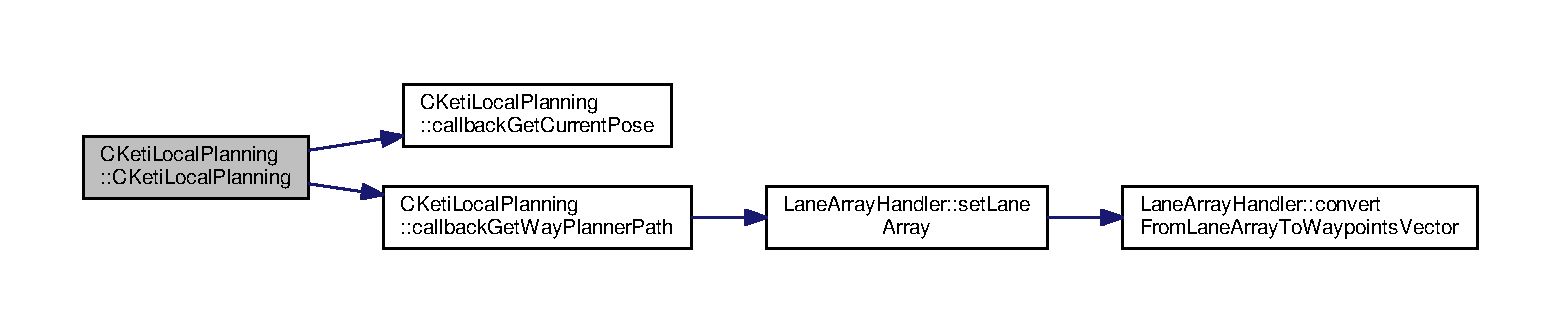
\includegraphics[width=350pt]{class_c_keti_local_planning_a64e789f070f7334aab7727c0ae276931_cgraph}
\end{center}
\end{figure}


\index{C\+Keti\+Local\+Planning@{C\+Keti\+Local\+Planning}!````~C\+Keti\+Local\+Planning@{$\sim$\+C\+Keti\+Local\+Planning}}
\index{````~C\+Keti\+Local\+Planning@{$\sim$\+C\+Keti\+Local\+Planning}!C\+Keti\+Local\+Planning@{C\+Keti\+Local\+Planning}}
\subsubsection[{\texorpdfstring{$\sim$\+C\+Keti\+Local\+Planning()}{~CKetiLocalPlanning()}}]{\setlength{\rightskip}{0pt plus 5cm}C\+Keti\+Local\+Planning\+::$\sim$\+C\+Keti\+Local\+Planning (
\begin{DoxyParamCaption}
{}
\end{DoxyParamCaption}
)}\hypertarget{class_c_keti_local_planning_adab5b7e3683328d05b50ed802e2fb5cd}{}\label{class_c_keti_local_planning_adab5b7e3683328d05b50ed802e2fb5cd}


cketilocalplanning.\+cpp 파일의 22 번째 라인에서 정의되었습니다.


\begin{DoxyCode}
23 \{
24 
25 \}
\end{DoxyCode}


\subsection{멤버 함수 문서화}
\index{C\+Keti\+Local\+Planning@{C\+Keti\+Local\+Planning}!callback\+Get\+Current\+Pose@{callback\+Get\+Current\+Pose}}
\index{callback\+Get\+Current\+Pose@{callback\+Get\+Current\+Pose}!C\+Keti\+Local\+Planning@{C\+Keti\+Local\+Planning}}
\subsubsection[{\texorpdfstring{callback\+Get\+Current\+Pose(const geometry\+\_\+msgs\+::\+Pose\+Stamped\+Const\+Ptr \&msg)}{callbackGetCurrentPose(const geometry_msgs::PoseStampedConstPtr &msg)}}]{\setlength{\rightskip}{0pt plus 5cm}void C\+Keti\+Local\+Planning\+::callback\+Get\+Current\+Pose (
\begin{DoxyParamCaption}
\item[{const geometry\+\_\+msgs\+::\+Pose\+Stamped\+Const\+Ptr \&}]{msg}
\end{DoxyParamCaption}
)\hspace{0.3cm}{\ttfamily [protected]}}\hypertarget{class_c_keti_local_planning_a144131de19f37584bab4412f98e1fc63}{}\label{class_c_keti_local_planning_a144131de19f37584bab4412f98e1fc63}


callback\+Get\+Current\+Pose 


\begin{DoxyParams}{매개변수}
{\em geometry\+\_\+msgs\+::\+Pose\+Stamped\+Const\+Ptr} & /current\+\_\+pose \\
\hline
\end{DoxyParams}


cketilocalplanning.\+cpp 파일의 28 번째 라인에서 정의되었습니다.


\begin{DoxyCode}
29 \{
30   \hyperlink{class_c_keti_local_planning_a4f4dcb94c250fb4d324b33f2fa42ffcb}{current\_pose\_} = msg->pose;
31 \}
\end{DoxyCode}


이 함수를 호출하는 함수들에 대한 그래프입니다.\+:\nopagebreak
\begin{figure}[H]
\begin{center}
\leavevmode
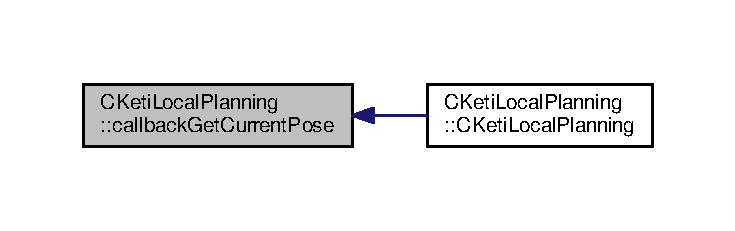
\includegraphics[width=350pt]{class_c_keti_local_planning_a144131de19f37584bab4412f98e1fc63_icgraph}
\end{center}
\end{figure}


\index{C\+Keti\+Local\+Planning@{C\+Keti\+Local\+Planning}!callback\+Get\+Way\+Planner\+Path@{callback\+Get\+Way\+Planner\+Path}}
\index{callback\+Get\+Way\+Planner\+Path@{callback\+Get\+Way\+Planner\+Path}!C\+Keti\+Local\+Planning@{C\+Keti\+Local\+Planning}}
\subsubsection[{\texorpdfstring{callback\+Get\+Way\+Planner\+Path(const autoware\+\_\+msgs\+::\+Lane\+Array \&msg)}{callbackGetWayPlannerPath(const autoware_msgs::LaneArray &msg)}}]{\setlength{\rightskip}{0pt plus 5cm}void C\+Keti\+Local\+Planning\+::callback\+Get\+Way\+Planner\+Path (
\begin{DoxyParamCaption}
\item[{const autoware\+\_\+msgs\+::\+Lane\+Array \&}]{msg}
\end{DoxyParamCaption}
)\hspace{0.3cm}{\ttfamily [protected]}}\hypertarget{class_c_keti_local_planning_ab385a1021d3d90f9f2b7b5a40dd791c2}{}\label{class_c_keti_local_planning_ab385a1021d3d90f9f2b7b5a40dd791c2}


callback\+Get\+Way\+Planner\+Path 


\begin{DoxyParams}{매개변수}
{\em autoware\+\_\+msgs\+::\+Lane\+Array\+Const\+Ptr} & /lane\+\_\+waypoints\+\_\+\+Array \\
\hline
\end{DoxyParams}


cketilocalplanning.\+cpp 파일의 33 번째 라인에서 정의되었습니다.


\begin{DoxyCode}
34 \{
35   \hyperlink{class_c_keti_local_planning_a6295120665288244397783d747cc60cf}{lanes\_handler\_}.\hyperlink{class_lane_array_handler_a345c18674ccfcbf1104bd5b030e04c0b}{setLaneArray}(msg);
36 \}
\end{DoxyCode}


이 함수 내부에서 호출하는 함수들에 대한 그래프입니다.\+:\nopagebreak
\begin{figure}[H]
\begin{center}
\leavevmode
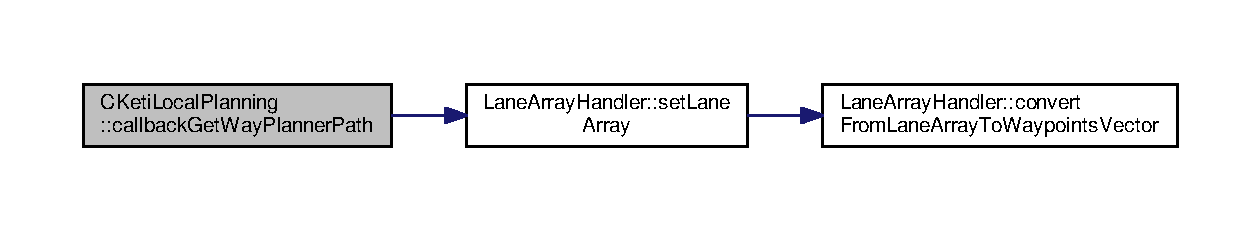
\includegraphics[width=350pt]{class_c_keti_local_planning_ab385a1021d3d90f9f2b7b5a40dd791c2_cgraph}
\end{center}
\end{figure}




이 함수를 호출하는 함수들에 대한 그래프입니다.\+:\nopagebreak
\begin{figure}[H]
\begin{center}
\leavevmode
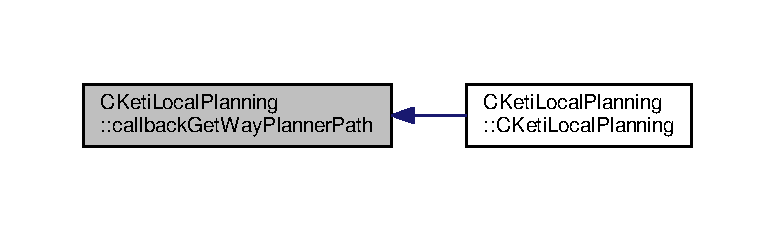
\includegraphics[width=350pt]{class_c_keti_local_planning_ab385a1021d3d90f9f2b7b5a40dd791c2_icgraph}
\end{center}
\end{figure}


\index{C\+Keti\+Local\+Planning@{C\+Keti\+Local\+Planning}!Planner\+Main\+Loop@{Planner\+Main\+Loop}}
\index{Planner\+Main\+Loop@{Planner\+Main\+Loop}!C\+Keti\+Local\+Planning@{C\+Keti\+Local\+Planning}}
\subsubsection[{\texorpdfstring{Planner\+Main\+Loop()}{PlannerMainLoop()}}]{\setlength{\rightskip}{0pt plus 5cm}void C\+Keti\+Local\+Planning\+::\+Planner\+Main\+Loop (
\begin{DoxyParamCaption}
{}
\end{DoxyParamCaption}
)}\hypertarget{class_c_keti_local_planning_a3286318e734e7441036b43cec169978c}{}\label{class_c_keti_local_planning_a3286318e734e7441036b43cec169978c}


cketilocalplanning.\+cpp 파일의 38 번째 라인에서 정의되었습니다.


\begin{DoxyCode}
39 \{
40   ros::Rate loop\_rate(100);
41 
42   \hyperlink{class_lane_handler}{LaneHandler} lane\_handler;
43 
44   \textcolor{keywordflow}{while} (ros::ok())
45   \{
46     \textcolor{keywordflow}{if}(\hyperlink{class_c_keti_local_planning_a6295120665288244397783d747cc60cf}{lanes\_handler\_}.\hyperlink{class_lane_array_handler_ab6fec5fc6f51e9b00949766093608b6f}{autoware\_lanearray\_}.lanes.empty())
47     \{
48       \textcolor{keywordflow}{continue};
49     \}\textcolor{keywordflow}{else}\{
50       lane\_handler.\hyperlink{class_lane_handler_a6c4cc7f5ae19a81cd24ba1427b0afb74}{setLane}(\hyperlink{class_c_keti_local_planning_a6295120665288244397783d747cc60cf}{lanes\_handler\_}.
      \hyperlink{class_lane_array_handler_ab6fec5fc6f51e9b00949766093608b6f}{autoware\_lanearray\_}.lanes.at(1));
51     \}
52     ros::spinOnce();
53     \textcolor{keywordtype}{int} closest\_waypoint\_number = lane\_handler.\hyperlink{class_lane_handler_a71033c4e67c07e09c2c3c18fabfb7463}{getClosestWaypoint}(
      \hyperlink{class_c_keti_local_planning_a4f4dcb94c250fb4d324b33f2fa42ffcb}{current\_pose\_});
54 
55     \textcolor{keywordflow}{if}(closest\_waypoint\_number == -1)\{
56       \textcolor{keywordflow}{continue};
57     \}
58     \textcolor{comment}{// out\_waypoints: local trajectory to be generated.}
59     \textcolor{comment}{// out\_trajectory: local trajectory to be published}
60     \textcolor{comment}{// Temperal Work: Generate local trajectory from 20 waypoints from the closest waypoint}
61     std::vector<WayPoint> out\_waypoints;
62     autoware\_msgs::lane out\_trajectory;
63     \textcolor{keywordflow}{if}(lane\_handler.\hyperlink{class_lane_handler_ac65a0139b3900a7c8dc3fe49d7a684f3}{waypoints\_lane\_}.size()-closest\_waypoint\_number>20)\{
64       out\_waypoints.insert(out\_waypoints.begin(),
65                            lane\_handler.\hyperlink{class_lane_handler_ac65a0139b3900a7c8dc3fe49d7a684f3}{waypoints\_lane\_}.begin()+closest\_waypoint\_number,
66                            lane\_handler.\hyperlink{class_lane_handler_ac65a0139b3900a7c8dc3fe49d7a684f3}{waypoints\_lane\_}.begin()+closest\_waypoint\_number+20);
67     \}\textcolor{keywordflow}{else}\{
68       out\_waypoints.insert(out\_waypoints.begin(),
69                            lane\_handler.\hyperlink{class_lane_handler_ac65a0139b3900a7c8dc3fe49d7a684f3}{waypoints\_lane\_}.begin()+closest\_waypoint\_number,
70                            lane\_handler.\hyperlink{class_lane_handler_ac65a0139b3900a7c8dc3fe49d7a684f3}{waypoints\_lane\_}.end());
71     \}
72     \hyperlink{class_lane_handler}{LaneHandler} out\_lane\_handler(out\_waypoints);
73     \hyperlink{class_c_keti_local_planning_a42f394ae6069296e6f412eb5daa9dd3a}{pub\_LocalPath}.publish(out\_lane\_handler.getAutowareLane());
74 
75     \textcolor{comment}{//Visualization for local path}
76     visualization\_msgs::MarkerArray local\_marker;
77     \hyperlink{class_ros_helpers_a00357e856ae16110fd9f3787cc3802d3}{RosHelpers::ConvertFromLocalPlannerHToAutowareVisualizePathFormat}
      (out\_waypoints,local\_marker);
78     \hyperlink{class_c_keti_local_planning_a423ed1137dde91f12793bdcacb4e0bea}{pub\_LocalTrajectoriesRviz}.publish(local\_marker);
79 
80     \textcolor{comment}{// Visualization for global path}
81     visualization\_msgs::MarkerArray waypoint\_marker;
82     \hyperlink{class_ros_helpers_ad82466a16ba11fded30d109a52b75074}{RosHelpers::ConvertFromPlannerHToAutowareVisualizePathFormat}
      (\hyperlink{class_c_keti_local_planning_a6295120665288244397783d747cc60cf}{lanes\_handler\_}.\hyperlink{class_lane_array_handler_a5f6a1e79b64a9092bfad57fd6676432b}{lanes\_},waypoint\_marker);
83     \hyperlink{class_c_keti_local_planning_a54aec2f11f157100a74b09a9cf5fa38b}{pub\_WaypointTrajectoriesRviz}.publish(waypoint\_marker);
84 
85 
86     loop\_rate.sleep();
87   \}
88 \}
\end{DoxyCode}


이 함수 내부에서 호출하는 함수들에 대한 그래프입니다.\+:\nopagebreak
\begin{figure}[H]
\begin{center}
\leavevmode
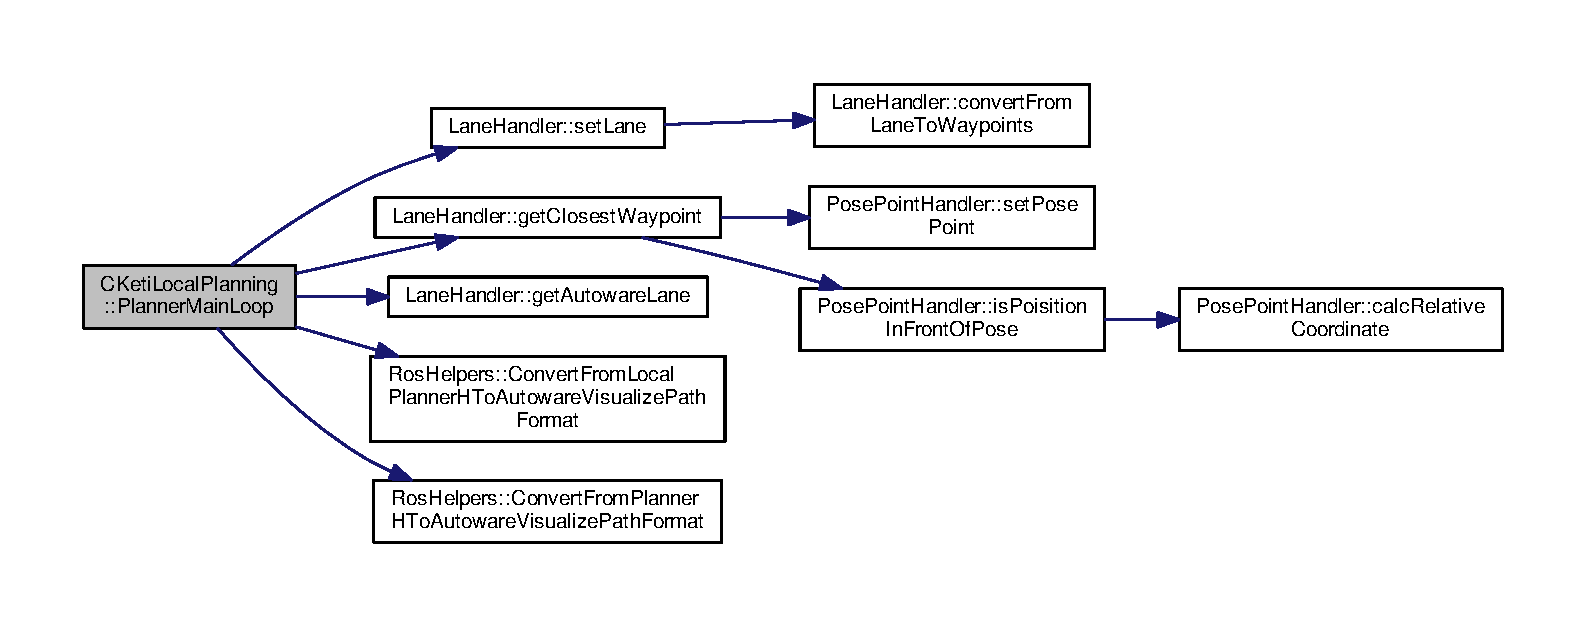
\includegraphics[width=350pt]{class_c_keti_local_planning_a3286318e734e7441036b43cec169978c_cgraph}
\end{center}
\end{figure}




이 함수를 호출하는 함수들에 대한 그래프입니다.\+:\nopagebreak
\begin{figure}[H]
\begin{center}
\leavevmode
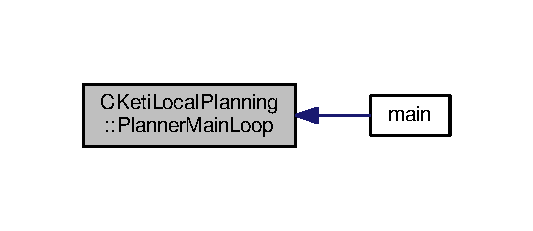
\includegraphics[width=256pt]{class_c_keti_local_planning_a3286318e734e7441036b43cec169978c_icgraph}
\end{center}
\end{figure}




\subsection{멤버 데이타 문서화}
\index{C\+Keti\+Local\+Planning@{C\+Keti\+Local\+Planning}!current\+\_\+pose\+\_\+@{current\+\_\+pose\+\_\+}}
\index{current\+\_\+pose\+\_\+@{current\+\_\+pose\+\_\+}!C\+Keti\+Local\+Planning@{C\+Keti\+Local\+Planning}}
\subsubsection[{\texorpdfstring{current\+\_\+pose\+\_\+}{current_pose_}}]{\setlength{\rightskip}{0pt plus 5cm}geometry\+\_\+msgs\+::\+Pose C\+Keti\+Local\+Planning\+::current\+\_\+pose\+\_\+\hspace{0.3cm}{\ttfamily [protected]}}\hypertarget{class_c_keti_local_planning_a4f4dcb94c250fb4d324b33f2fa42ffcb}{}\label{class_c_keti_local_planning_a4f4dcb94c250fb4d324b33f2fa42ffcb}


cketilocalplanning.\+h 파일의 29 번째 라인에서 정의되었습니다.

\index{C\+Keti\+Local\+Planning@{C\+Keti\+Local\+Planning}!lanes\+\_\+handler\+\_\+@{lanes\+\_\+handler\+\_\+}}
\index{lanes\+\_\+handler\+\_\+@{lanes\+\_\+handler\+\_\+}!C\+Keti\+Local\+Planning@{C\+Keti\+Local\+Planning}}
\subsubsection[{\texorpdfstring{lanes\+\_\+handler\+\_\+}{lanes_handler_}}]{\setlength{\rightskip}{0pt plus 5cm}{\bf Lane\+Array\+Handler} C\+Keti\+Local\+Planning\+::lanes\+\_\+handler\+\_\+\hspace{0.3cm}{\ttfamily [protected]}}\hypertarget{class_c_keti_local_planning_a6295120665288244397783d747cc60cf}{}\label{class_c_keti_local_planning_a6295120665288244397783d747cc60cf}


cketilocalplanning.\+h 파일의 30 번째 라인에서 정의되었습니다.

\index{C\+Keti\+Local\+Planning@{C\+Keti\+Local\+Planning}!nh@{nh}}
\index{nh@{nh}!C\+Keti\+Local\+Planning@{C\+Keti\+Local\+Planning}}
\subsubsection[{\texorpdfstring{nh}{nh}}]{\setlength{\rightskip}{0pt plus 5cm}ros\+::\+Node\+Handle C\+Keti\+Local\+Planning\+::nh\hspace{0.3cm}{\ttfamily [protected]}}\hypertarget{class_c_keti_local_planning_a39a260e89fa7805f6c0c7112c91cb847}{}\label{class_c_keti_local_planning_a39a260e89fa7805f6c0c7112c91cb847}


cketilocalplanning.\+h 파일의 22 번째 라인에서 정의되었습니다.

\index{C\+Keti\+Local\+Planning@{C\+Keti\+Local\+Planning}!pub\+\_\+\+Local\+Path@{pub\+\_\+\+Local\+Path}}
\index{pub\+\_\+\+Local\+Path@{pub\+\_\+\+Local\+Path}!C\+Keti\+Local\+Planning@{C\+Keti\+Local\+Planning}}
\subsubsection[{\texorpdfstring{pub\+\_\+\+Local\+Path}{pub_LocalPath}}]{\setlength{\rightskip}{0pt plus 5cm}ros\+::\+Publisher C\+Keti\+Local\+Planning\+::pub\+\_\+\+Local\+Path\hspace{0.3cm}{\ttfamily [protected]}}\hypertarget{class_c_keti_local_planning_a42f394ae6069296e6f412eb5daa9dd3a}{}\label{class_c_keti_local_planning_a42f394ae6069296e6f412eb5daa9dd3a}


cketilocalplanning.\+h 파일의 23 번째 라인에서 정의되었습니다.

\index{C\+Keti\+Local\+Planning@{C\+Keti\+Local\+Planning}!pub\+\_\+\+Local\+Trajectories\+Rviz@{pub\+\_\+\+Local\+Trajectories\+Rviz}}
\index{pub\+\_\+\+Local\+Trajectories\+Rviz@{pub\+\_\+\+Local\+Trajectories\+Rviz}!C\+Keti\+Local\+Planning@{C\+Keti\+Local\+Planning}}
\subsubsection[{\texorpdfstring{pub\+\_\+\+Local\+Trajectories\+Rviz}{pub_LocalTrajectoriesRviz}}]{\setlength{\rightskip}{0pt plus 5cm}ros\+::\+Publisher C\+Keti\+Local\+Planning\+::pub\+\_\+\+Local\+Trajectories\+Rviz\hspace{0.3cm}{\ttfamily [protected]}}\hypertarget{class_c_keti_local_planning_a423ed1137dde91f12793bdcacb4e0bea}{}\label{class_c_keti_local_planning_a423ed1137dde91f12793bdcacb4e0bea}


cketilocalplanning.\+h 파일의 24 번째 라인에서 정의되었습니다.

\index{C\+Keti\+Local\+Planning@{C\+Keti\+Local\+Planning}!pub\+\_\+\+Waypoint\+Trajectories\+Rviz@{pub\+\_\+\+Waypoint\+Trajectories\+Rviz}}
\index{pub\+\_\+\+Waypoint\+Trajectories\+Rviz@{pub\+\_\+\+Waypoint\+Trajectories\+Rviz}!C\+Keti\+Local\+Planning@{C\+Keti\+Local\+Planning}}
\subsubsection[{\texorpdfstring{pub\+\_\+\+Waypoint\+Trajectories\+Rviz}{pub_WaypointTrajectoriesRviz}}]{\setlength{\rightskip}{0pt plus 5cm}ros\+::\+Publisher C\+Keti\+Local\+Planning\+::pub\+\_\+\+Waypoint\+Trajectories\+Rviz\hspace{0.3cm}{\ttfamily [protected]}}\hypertarget{class_c_keti_local_planning_a54aec2f11f157100a74b09a9cf5fa38b}{}\label{class_c_keti_local_planning_a54aec2f11f157100a74b09a9cf5fa38b}


cketilocalplanning.\+h 파일의 25 번째 라인에서 정의되었습니다.

\index{C\+Keti\+Local\+Planning@{C\+Keti\+Local\+Planning}!sub\+\_\+current\+\_\+pose@{sub\+\_\+current\+\_\+pose}}
\index{sub\+\_\+current\+\_\+pose@{sub\+\_\+current\+\_\+pose}!C\+Keti\+Local\+Planning@{C\+Keti\+Local\+Planning}}
\subsubsection[{\texorpdfstring{sub\+\_\+current\+\_\+pose}{sub_current_pose}}]{\setlength{\rightskip}{0pt plus 5cm}ros\+::\+Subscriber C\+Keti\+Local\+Planning\+::sub\+\_\+current\+\_\+pose\hspace{0.3cm}{\ttfamily [protected]}}\hypertarget{class_c_keti_local_planning_ac399c600a59f7b79448ba1f1bbfda8ca}{}\label{class_c_keti_local_planning_ac399c600a59f7b79448ba1f1bbfda8ca}


cketilocalplanning.\+h 파일의 26 번째 라인에서 정의되었습니다.

\index{C\+Keti\+Local\+Planning@{C\+Keti\+Local\+Planning}!sub\+\_\+\+Way\+Planner\+Paths@{sub\+\_\+\+Way\+Planner\+Paths}}
\index{sub\+\_\+\+Way\+Planner\+Paths@{sub\+\_\+\+Way\+Planner\+Paths}!C\+Keti\+Local\+Planning@{C\+Keti\+Local\+Planning}}
\subsubsection[{\texorpdfstring{sub\+\_\+\+Way\+Planner\+Paths}{sub_WayPlannerPaths}}]{\setlength{\rightskip}{0pt plus 5cm}ros\+::\+Subscriber C\+Keti\+Local\+Planning\+::sub\+\_\+\+Way\+Planner\+Paths\hspace{0.3cm}{\ttfamily [protected]}}\hypertarget{class_c_keti_local_planning_a75e59488889af86a89995f2c606677ce}{}\label{class_c_keti_local_planning_a75e59488889af86a89995f2c606677ce}


cketilocalplanning.\+h 파일의 27 번째 라인에서 정의되었습니다.



이 클래스에 대한 문서화 페이지는 다음의 파일들로부터 생성되었습니다.\+:\begin{DoxyCompactItemize}
\item 
/home/dallddungi/keti\+\_\+ws/src/keti\+\_\+local\+\_\+planning/include/\hyperlink{cketilocalplanning_8h}{cketilocalplanning.\+h}\item 
/home/dallddungi/keti\+\_\+ws/src/keti\+\_\+local\+\_\+planning/src/\hyperlink{cketilocalplanning_8cpp}{cketilocalplanning.\+cpp}\end{DoxyCompactItemize}

\hypertarget{class_g_p_s_point}{}\section{G\+P\+S\+Point 클래스 참조}
\label{class_g_p_s_point}\index{G\+P\+S\+Point@{G\+P\+S\+Point}}


type representing class containing (x,y,z,a)  




{\ttfamily \#include $<$gpspoint.\+h$>$}



G\+P\+S\+Point에 대한 협력 다이어그램\+:\nopagebreak
\begin{figure}[H]
\begin{center}
\leavevmode
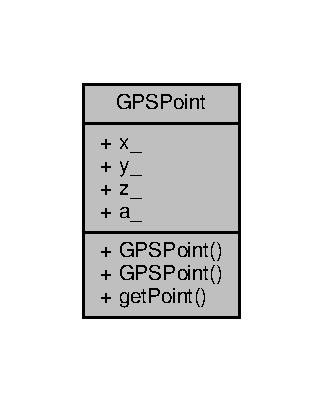
\includegraphics[width=155pt]{class_g_p_s_point__coll__graph}
\end{center}
\end{figure}
\subsection*{Public 멤버 함수}
\begin{DoxyCompactItemize}
\item 
\hyperlink{class_g_p_s_point_a7a635f12f124e516210755b0974ee1d4}{G\+P\+S\+Point} ()
\item 
\hyperlink{class_g_p_s_point_aab0d3a5aaee6586b615f55a82c17a10d}{G\+P\+S\+Point} (const double \&x, const double \&y, const double \&z, const double \&a)
\item 
geometry\+\_\+msgs\+::\+Point \hyperlink{class_g_p_s_point_aa02789544161ef0bcc40a24972f1b365}{get\+Point} ()
\end{DoxyCompactItemize}
\subsection*{Public 속성}
\begin{DoxyCompactItemize}
\item 
double \hyperlink{class_g_p_s_point_ad4b7325afe1ca0fcf8d2ef284ab9b62c}{x\+\_\+}
\item 
double \hyperlink{class_g_p_s_point_ad41d0e7a93f8766181402ce25af798fe}{y\+\_\+}
\item 
double \hyperlink{class_g_p_s_point_aa6622ef5c0c58fa1b59c1d5b77fe020c}{z\+\_\+}
\item 
double \hyperlink{class_g_p_s_point_ac4652d53d65aeb605f7eb35128a5ab90}{a\+\_\+}
\end{DoxyCompactItemize}


\subsection{상세한 설명}
type representing class containing (x,y,z,a) 

gpspoint.\+h 파일의 10 번째 라인에서 정의되었습니다.



\subsection{생성자 \& 소멸자 문서화}
\index{G\+P\+S\+Point@{G\+P\+S\+Point}!G\+P\+S\+Point@{G\+P\+S\+Point}}
\index{G\+P\+S\+Point@{G\+P\+S\+Point}!G\+P\+S\+Point@{G\+P\+S\+Point}}
\subsubsection[{\texorpdfstring{G\+P\+S\+Point()}{GPSPoint()}}]{\setlength{\rightskip}{0pt plus 5cm}G\+P\+S\+Point\+::\+G\+P\+S\+Point (
\begin{DoxyParamCaption}
{}
\end{DoxyParamCaption}
)\hspace{0.3cm}{\ttfamily [inline]}}\hypertarget{class_g_p_s_point_a7a635f12f124e516210755b0974ee1d4}{}\label{class_g_p_s_point_a7a635f12f124e516210755b0974ee1d4}


gpspoint.\+h 파일의 18 번째 라인에서 정의되었습니다.


\begin{DoxyCode}
19   \{
20     \hyperlink{class_g_p_s_point_ad4b7325afe1ca0fcf8d2ef284ab9b62c}{x\_} = 0;
21     \hyperlink{class_g_p_s_point_ad41d0e7a93f8766181402ce25af798fe}{y\_} = 0;
22     \hyperlink{class_g_p_s_point_aa6622ef5c0c58fa1b59c1d5b77fe020c}{z\_} = 0;
23     \hyperlink{class_g_p_s_point_ac4652d53d65aeb605f7eb35128a5ab90}{a\_} = 0;
24   \}
\end{DoxyCode}
\index{G\+P\+S\+Point@{G\+P\+S\+Point}!G\+P\+S\+Point@{G\+P\+S\+Point}}
\index{G\+P\+S\+Point@{G\+P\+S\+Point}!G\+P\+S\+Point@{G\+P\+S\+Point}}
\subsubsection[{\texorpdfstring{G\+P\+S\+Point(const double \&x, const double \&y, const double \&z, const double \&a)}{GPSPoint(const double &x, const double &y, const double &z, const double &a)}}]{\setlength{\rightskip}{0pt plus 5cm}G\+P\+S\+Point\+::\+G\+P\+S\+Point (
\begin{DoxyParamCaption}
\item[{const double \&}]{x, }
\item[{const double \&}]{y, }
\item[{const double \&}]{z, }
\item[{const double \&}]{a}
\end{DoxyParamCaption}
)\hspace{0.3cm}{\ttfamily [inline]}}\hypertarget{class_g_p_s_point_aab0d3a5aaee6586b615f55a82c17a10d}{}\label{class_g_p_s_point_aab0d3a5aaee6586b615f55a82c17a10d}


gpspoint.\+h 파일의 26 번째 라인에서 정의되었습니다.


\begin{DoxyCode}
27   \{
28     this->\hyperlink{class_g_p_s_point_ad4b7325afe1ca0fcf8d2ef284ab9b62c}{x\_} = x;
29     this->\hyperlink{class_g_p_s_point_ad41d0e7a93f8766181402ce25af798fe}{y\_} = y;
30     this->\hyperlink{class_g_p_s_point_aa6622ef5c0c58fa1b59c1d5b77fe020c}{z\_} = z;
31     this->\hyperlink{class_g_p_s_point_ac4652d53d65aeb605f7eb35128a5ab90}{a\_} = a;
32 
33   \}
\end{DoxyCode}


\subsection{멤버 함수 문서화}
\index{G\+P\+S\+Point@{G\+P\+S\+Point}!get\+Point@{get\+Point}}
\index{get\+Point@{get\+Point}!G\+P\+S\+Point@{G\+P\+S\+Point}}
\subsubsection[{\texorpdfstring{get\+Point()}{getPoint()}}]{\setlength{\rightskip}{0pt plus 5cm}geometry\+\_\+msgs\+::\+Point G\+P\+S\+Point\+::get\+Point (
\begin{DoxyParamCaption}
{}
\end{DoxyParamCaption}
)\hspace{0.3cm}{\ttfamily [inline]}}\hypertarget{class_g_p_s_point_aa02789544161ef0bcc40a24972f1b365}{}\label{class_g_p_s_point_aa02789544161ef0bcc40a24972f1b365}


gpspoint.\+h 파일의 35 번째 라인에서 정의되었습니다.


\begin{DoxyCode}
36   \{
37     geometry\_msgs::Point pt;
38     pt.x = \hyperlink{class_g_p_s_point_ad4b7325afe1ca0fcf8d2ef284ab9b62c}{x\_};
39     pt.y = \hyperlink{class_g_p_s_point_ad41d0e7a93f8766181402ce25af798fe}{y\_};
40     pt.z = \hyperlink{class_g_p_s_point_aa6622ef5c0c58fa1b59c1d5b77fe020c}{z\_};
41     \textcolor{keywordflow}{return} pt;
42   \}
\end{DoxyCode}


\subsection{멤버 데이타 문서화}
\index{G\+P\+S\+Point@{G\+P\+S\+Point}!a\+\_\+@{a\+\_\+}}
\index{a\+\_\+@{a\+\_\+}!G\+P\+S\+Point@{G\+P\+S\+Point}}
\subsubsection[{\texorpdfstring{a\+\_\+}{a_}}]{\setlength{\rightskip}{0pt plus 5cm}double G\+P\+S\+Point\+::a\+\_\+}\hypertarget{class_g_p_s_point_ac4652d53d65aeb605f7eb35128a5ab90}{}\label{class_g_p_s_point_ac4652d53d65aeb605f7eb35128a5ab90}


gpspoint.\+h 파일의 16 번째 라인에서 정의되었습니다.

\index{G\+P\+S\+Point@{G\+P\+S\+Point}!x\+\_\+@{x\+\_\+}}
\index{x\+\_\+@{x\+\_\+}!G\+P\+S\+Point@{G\+P\+S\+Point}}
\subsubsection[{\texorpdfstring{x\+\_\+}{x_}}]{\setlength{\rightskip}{0pt plus 5cm}double G\+P\+S\+Point\+::x\+\_\+}\hypertarget{class_g_p_s_point_ad4b7325afe1ca0fcf8d2ef284ab9b62c}{}\label{class_g_p_s_point_ad4b7325afe1ca0fcf8d2ef284ab9b62c}


gpspoint.\+h 파일의 13 번째 라인에서 정의되었습니다.

\index{G\+P\+S\+Point@{G\+P\+S\+Point}!y\+\_\+@{y\+\_\+}}
\index{y\+\_\+@{y\+\_\+}!G\+P\+S\+Point@{G\+P\+S\+Point}}
\subsubsection[{\texorpdfstring{y\+\_\+}{y_}}]{\setlength{\rightskip}{0pt plus 5cm}double G\+P\+S\+Point\+::y\+\_\+}\hypertarget{class_g_p_s_point_ad41d0e7a93f8766181402ce25af798fe}{}\label{class_g_p_s_point_ad41d0e7a93f8766181402ce25af798fe}


gpspoint.\+h 파일의 14 번째 라인에서 정의되었습니다.

\index{G\+P\+S\+Point@{G\+P\+S\+Point}!z\+\_\+@{z\+\_\+}}
\index{z\+\_\+@{z\+\_\+}!G\+P\+S\+Point@{G\+P\+S\+Point}}
\subsubsection[{\texorpdfstring{z\+\_\+}{z_}}]{\setlength{\rightskip}{0pt plus 5cm}double G\+P\+S\+Point\+::z\+\_\+}\hypertarget{class_g_p_s_point_aa6622ef5c0c58fa1b59c1d5b77fe020c}{}\label{class_g_p_s_point_aa6622ef5c0c58fa1b59c1d5b77fe020c}


gpspoint.\+h 파일의 15 번째 라인에서 정의되었습니다.



이 클래스에 대한 문서화 페이지는 다음의 파일로부터 생성되었습니다.\+:\begin{DoxyCompactItemize}
\item 
/home/dallddungi/keti\+\_\+ws/src/keti\+\_\+local\+\_\+planning/include/data\+\_\+classes/\hyperlink{gpspoint_8h}{gpspoint.\+h}\end{DoxyCompactItemize}

\hypertarget{class_lane_array_handler}{}\section{Lane\+Array\+Handler 클래스 참조}
\label{class_lane_array_handler}\index{Lane\+Array\+Handler@{Lane\+Array\+Handler}}


The Type\+Conversion class This class is handling lane array information.  




{\ttfamily \#include $<$lanearray\+\_\+handler.\+h$>$}



Lane\+Array\+Handler에 대한 협력 다이어그램\+:\nopagebreak
\begin{figure}[H]
\begin{center}
\leavevmode
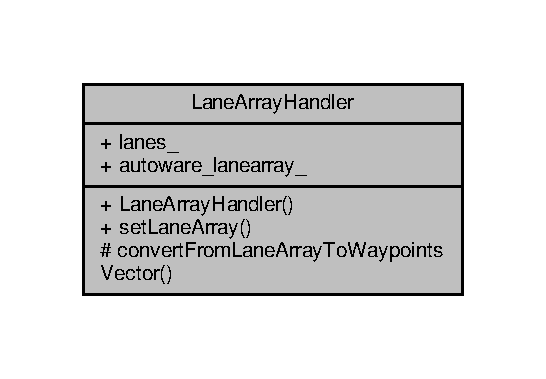
\includegraphics[width=262pt]{class_lane_array_handler__coll__graph}
\end{center}
\end{figure}
\subsection*{Public 멤버 함수}
\begin{DoxyCompactItemize}
\item 
\hyperlink{class_lane_array_handler_a5ffda8b0667a0b1060b4efe8d07789e1}{Lane\+Array\+Handler} ()
\item 
void \hyperlink{class_lane_array_handler_a345c18674ccfcbf1104bd5b030e04c0b}{set\+Lane\+Array} (const autoware\+\_\+msgs\+::\+Lane\+Array \&lane\+\_\+array)
\end{DoxyCompactItemize}
\subsection*{Public 속성}
\begin{DoxyCompactItemize}
\item 
std\+::vector$<$ std\+::vector$<$ \hyperlink{class_way_point}{Way\+Point} $>$ $>$ \hyperlink{class_lane_array_handler_a5f6a1e79b64a9092bfad57fd6676432b}{lanes\+\_\+}
\item 
autoware\+\_\+msgs\+::\+Lane\+Array \hyperlink{class_lane_array_handler_ab6fec5fc6f51e9b00949766093608b6f}{autoware\+\_\+lanearray\+\_\+}
\end{DoxyCompactItemize}
\subsection*{Protected 멤버 함수}
\begin{DoxyCompactItemize}
\item 
std\+::vector$<$ std\+::vector$<$ \hyperlink{class_way_point}{Way\+Point} $>$ $>$ \hyperlink{class_lane_array_handler_a24dff427e3c72bb3a26cdcc44c718044}{convert\+From\+Lane\+Array\+To\+Waypoints\+Vector} (const autoware\+\_\+msgs\+::\+Lane\+Array \&lane\+\_\+array)
\end{DoxyCompactItemize}


\subsection{상세한 설명}
The Type\+Conversion class This class is handling lane array information. 

lanearray\+\_\+handler.\+h 파일의 15 번째 라인에서 정의되었습니다.



\subsection{생성자 \& 소멸자 문서화}
\index{Lane\+Array\+Handler@{Lane\+Array\+Handler}!Lane\+Array\+Handler@{Lane\+Array\+Handler}}
\index{Lane\+Array\+Handler@{Lane\+Array\+Handler}!Lane\+Array\+Handler@{Lane\+Array\+Handler}}
\subsubsection[{\texorpdfstring{Lane\+Array\+Handler()}{LaneArrayHandler()}}]{\setlength{\rightskip}{0pt plus 5cm}Lane\+Array\+Handler\+::\+Lane\+Array\+Handler (
\begin{DoxyParamCaption}
{}
\end{DoxyParamCaption}
)}\hypertarget{class_lane_array_handler_a5ffda8b0667a0b1060b4efe8d07789e1}{}\label{class_lane_array_handler_a5ffda8b0667a0b1060b4efe8d07789e1}


lanearray\+\_\+handler.\+cpp 파일의 4 번째 라인에서 정의되었습니다.


\begin{DoxyCode}
5 \{
6 
7 \}
\end{DoxyCode}


\subsection{멤버 함수 문서화}
\index{Lane\+Array\+Handler@{Lane\+Array\+Handler}!convert\+From\+Lane\+Array\+To\+Waypoints\+Vector@{convert\+From\+Lane\+Array\+To\+Waypoints\+Vector}}
\index{convert\+From\+Lane\+Array\+To\+Waypoints\+Vector@{convert\+From\+Lane\+Array\+To\+Waypoints\+Vector}!Lane\+Array\+Handler@{Lane\+Array\+Handler}}
\subsubsection[{\texorpdfstring{convert\+From\+Lane\+Array\+To\+Waypoints\+Vector(const autoware\+\_\+msgs\+::\+Lane\+Array \&lane\+\_\+array)}{convertFromLaneArrayToWaypointsVector(const autoware_msgs::LaneArray &lane_array)}}]{\setlength{\rightskip}{0pt plus 5cm}std\+::vector$<$ std\+::vector$<$ {\bf Way\+Point} $>$ $>$ Lane\+Array\+Handler\+::convert\+From\+Lane\+Array\+To\+Waypoints\+Vector (
\begin{DoxyParamCaption}
\item[{const autoware\+\_\+msgs\+::\+Lane\+Array \&}]{lane\+\_\+array}
\end{DoxyParamCaption}
)\hspace{0.3cm}{\ttfamily [protected]}}\hypertarget{class_lane_array_handler_a24dff427e3c72bb3a26cdcc44c718044}{}\label{class_lane_array_handler_a24dff427e3c72bb3a26cdcc44c718044}


lanearray\+\_\+handler.\+cpp 파일의 13 번째 라인에서 정의되었습니다.


\begin{DoxyCode}
14 \{
15   std::vector<std::vector<WayPoint> > paths;
16   \textcolor{keywordflow}{for}(\textcolor{keywordtype}{unsigned} \textcolor{keywordtype}{int} i = 0 ; i < lane\_array.lanes.size(); i++)
17   \{
18     std::vector<WayPoint> path;
19     \textcolor{keywordflow}{for}(\textcolor{keywordtype}{unsigned} \textcolor{keywordtype}{int} j = 0 ; j < lane\_array.lanes.at(i).waypoints.size(); j++)
20     \{
21       \hyperlink{class_way_point}{WayPoint} wp(lane\_array.lanes.at(i).waypoints.at(j).pose.pose.position.x,
22                   lane\_array.lanes.at(i).waypoints.at(j).pose.pose.position.y,
23                   lane\_array.lanes.at(i).waypoints.at(j).pose.pose.position.z,
24                   tf::getYaw(lane\_array.lanes.at(i).waypoints.at(j).pose.pose.orientation));
25       wp.v\_ = lane\_array.lanes.at(i).waypoints.at(j).twist.twist.linear.x;
26       path.push\_back(wp);
27     \}
28     paths.push\_back(path);
29   \}
30   \textcolor{keywordflow}{return} paths;
31 \}
\end{DoxyCode}


이 함수를 호출하는 함수들에 대한 그래프입니다.\+:\nopagebreak
\begin{figure}[H]
\begin{center}
\leavevmode
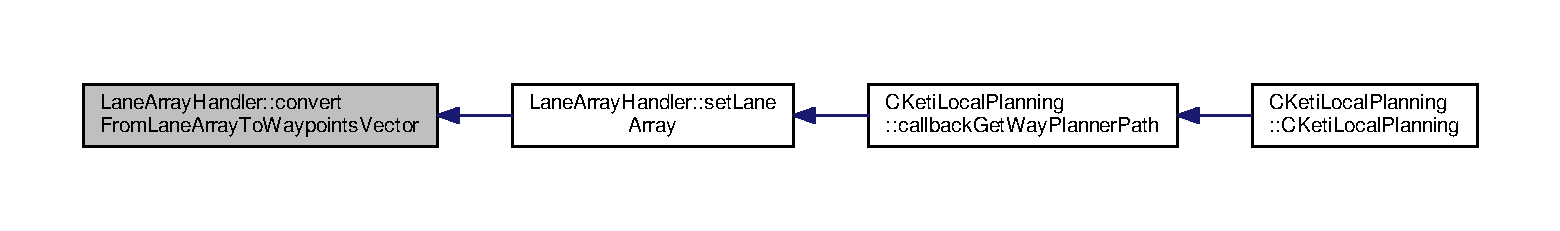
\includegraphics[width=350pt]{class_lane_array_handler_a24dff427e3c72bb3a26cdcc44c718044_icgraph}
\end{center}
\end{figure}


\index{Lane\+Array\+Handler@{Lane\+Array\+Handler}!set\+Lane\+Array@{set\+Lane\+Array}}
\index{set\+Lane\+Array@{set\+Lane\+Array}!Lane\+Array\+Handler@{Lane\+Array\+Handler}}
\subsubsection[{\texorpdfstring{set\+Lane\+Array(const autoware\+\_\+msgs\+::\+Lane\+Array \&lane\+\_\+array)}{setLaneArray(const autoware_msgs::LaneArray &lane_array)}}]{\setlength{\rightskip}{0pt plus 5cm}void Lane\+Array\+Handler\+::set\+Lane\+Array (
\begin{DoxyParamCaption}
\item[{const autoware\+\_\+msgs\+::\+Lane\+Array \&}]{lane\+\_\+array}
\end{DoxyParamCaption}
)}\hypertarget{class_lane_array_handler_a345c18674ccfcbf1104bd5b030e04c0b}{}\label{class_lane_array_handler_a345c18674ccfcbf1104bd5b030e04c0b}


lanearray\+\_\+handler.\+cpp 파일의 8 번째 라인에서 정의되었습니다.


\begin{DoxyCode}
9 \{
10   \hyperlink{class_lane_array_handler_a5f6a1e79b64a9092bfad57fd6676432b}{lanes\_} = \hyperlink{class_lane_array_handler_a24dff427e3c72bb3a26cdcc44c718044}{convertFromLaneArrayToWaypointsVector}(lane\_array);
11   \hyperlink{class_lane_array_handler_ab6fec5fc6f51e9b00949766093608b6f}{autoware\_lanearray\_} = lane\_array;
12 \}
\end{DoxyCode}


이 함수 내부에서 호출하는 함수들에 대한 그래프입니다.\+:\nopagebreak
\begin{figure}[H]
\begin{center}
\leavevmode
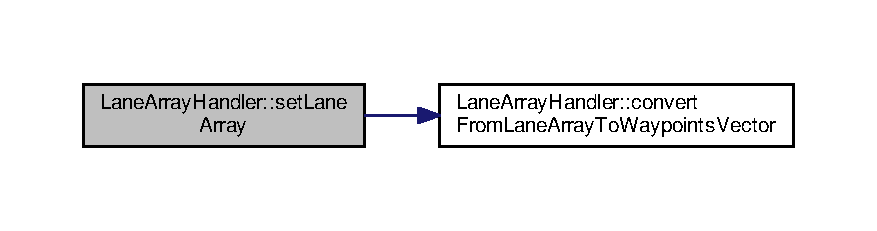
\includegraphics[width=350pt]{class_lane_array_handler_a345c18674ccfcbf1104bd5b030e04c0b_cgraph}
\end{center}
\end{figure}




이 함수를 호출하는 함수들에 대한 그래프입니다.\+:\nopagebreak
\begin{figure}[H]
\begin{center}
\leavevmode
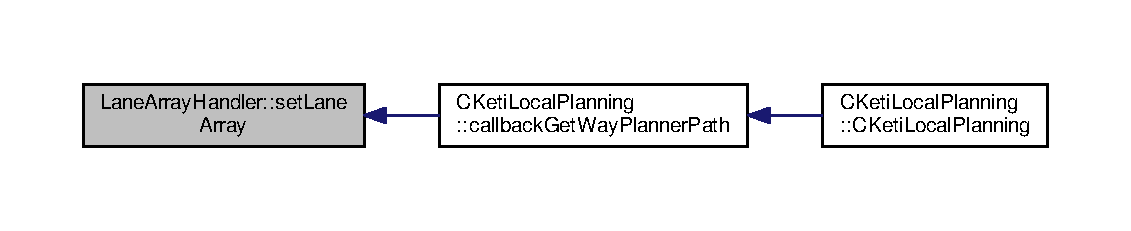
\includegraphics[width=350pt]{class_lane_array_handler_a345c18674ccfcbf1104bd5b030e04c0b_icgraph}
\end{center}
\end{figure}




\subsection{멤버 데이타 문서화}
\index{Lane\+Array\+Handler@{Lane\+Array\+Handler}!autoware\+\_\+lanearray\+\_\+@{autoware\+\_\+lanearray\+\_\+}}
\index{autoware\+\_\+lanearray\+\_\+@{autoware\+\_\+lanearray\+\_\+}!Lane\+Array\+Handler@{Lane\+Array\+Handler}}
\subsubsection[{\texorpdfstring{autoware\+\_\+lanearray\+\_\+}{autoware_lanearray_}}]{\setlength{\rightskip}{0pt plus 5cm}autoware\+\_\+msgs\+::\+Lane\+Array Lane\+Array\+Handler\+::autoware\+\_\+lanearray\+\_\+}\hypertarget{class_lane_array_handler_ab6fec5fc6f51e9b00949766093608b6f}{}\label{class_lane_array_handler_ab6fec5fc6f51e9b00949766093608b6f}


lanearray\+\_\+handler.\+h 파일의 20 번째 라인에서 정의되었습니다.

\index{Lane\+Array\+Handler@{Lane\+Array\+Handler}!lanes\+\_\+@{lanes\+\_\+}}
\index{lanes\+\_\+@{lanes\+\_\+}!Lane\+Array\+Handler@{Lane\+Array\+Handler}}
\subsubsection[{\texorpdfstring{lanes\+\_\+}{lanes_}}]{\setlength{\rightskip}{0pt plus 5cm}std\+::vector$<$std\+::vector$<${\bf Way\+Point}$>$ $>$ Lane\+Array\+Handler\+::lanes\+\_\+}\hypertarget{class_lane_array_handler_a5f6a1e79b64a9092bfad57fd6676432b}{}\label{class_lane_array_handler_a5f6a1e79b64a9092bfad57fd6676432b}


lanearray\+\_\+handler.\+h 파일의 19 번째 라인에서 정의되었습니다.



이 클래스에 대한 문서화 페이지는 다음의 파일들로부터 생성되었습니다.\+:\begin{DoxyCompactItemize}
\item 
/home/dallddungi/keti\+\_\+ws/src/keti\+\_\+local\+\_\+planning/include/data\+\_\+handler/\hyperlink{lanearray__handler_8h}{lanearray\+\_\+handler.\+h}\item 
/home/dallddungi/keti\+\_\+ws/src/keti\+\_\+local\+\_\+planning/src/data\+\_\+handler/\hyperlink{lanearray__handler_8cpp}{lanearray\+\_\+handler.\+cpp}\end{DoxyCompactItemize}

\hypertarget{class_lane_handler}{}\section{Lane\+Handler 클래스 참조}
\label{class_lane_handler}\index{Lane\+Handler@{Lane\+Handler}}


This class treats lane information with autowar\+\_\+msgs\+::lane and std\+::vector$<$\+Way\+Point$>$  




{\ttfamily \#include $<$lane\+\_\+handler.\+h$>$}



Lane\+Handler에 대한 협력 다이어그램\+:\nopagebreak
\begin{figure}[H]
\begin{center}
\leavevmode
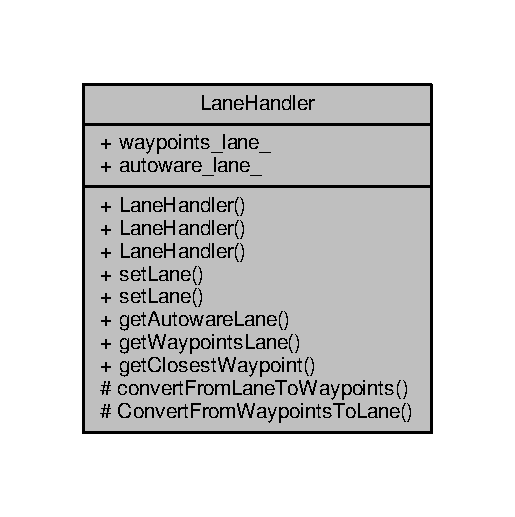
\includegraphics[width=247pt]{class_lane_handler__coll__graph}
\end{center}
\end{figure}
\subsection*{Public 멤버 함수}
\begin{DoxyCompactItemize}
\item 
\hyperlink{class_lane_handler_ac8a26880811b795d49d9b3578d3f03fb}{Lane\+Handler} ()
\item 
\hyperlink{class_lane_handler_af9236889af0e7d75ca3230d47175a9b5}{Lane\+Handler} (const std\+::vector$<$ \hyperlink{class_way_point}{Way\+Point} $>$ \&lane)
\item 
\hyperlink{class_lane_handler_af00842c287a4ea45b48a0d928b861048}{Lane\+Handler} (const autoware\+\_\+msgs\+::lane \&lane)
\item 
void \hyperlink{class_lane_handler_a6c4cc7f5ae19a81cd24ba1427b0afb74}{set\+Lane} (const autoware\+\_\+msgs\+::lane \&lane)
\item 
void \hyperlink{class_lane_handler_a33776b288c92ee7e63f865e6c9526ff3}{set\+Lane} (const std\+::vector$<$ \hyperlink{class_way_point}{Way\+Point} $>$ \&lane)
\item 
autoware\+\_\+msgs\+::lane \hyperlink{class_lane_handler_a9d66775c597130ccbd369d50c7572c2e}{get\+Autoware\+Lane} ()
\item 
std\+::vector$<$ \hyperlink{class_way_point}{Way\+Point} $>$ \hyperlink{class_lane_handler_afe241272b5017d7d0e439d08bbf855d9}{get\+Waypoints\+Lane} ()
\item 
int \hyperlink{class_lane_handler_a71033c4e67c07e09c2c3c18fabfb7463}{get\+Closest\+Waypoint} (const geometry\+\_\+msgs\+::\+Pose \&wp)
\begin{DoxyCompactList}\small\item\em Find a point on the lane which is the closest point to the \hyperlink{class_way_point}{Way\+Point}. \end{DoxyCompactList}\end{DoxyCompactItemize}
\subsection*{Public 속성}
\begin{DoxyCompactItemize}
\item 
std\+::vector$<$ \hyperlink{class_way_point}{Way\+Point} $>$ \hyperlink{class_lane_handler_ac65a0139b3900a7c8dc3fe49d7a684f3}{waypoints\+\_\+lane\+\_\+}
\item 
autoware\+\_\+msgs\+::lane \hyperlink{class_lane_handler_a167378a780eafb8242f7b12bd5460ac0}{autoware\+\_\+lane\+\_\+}
\end{DoxyCompactItemize}
\subsection*{Protected 멤버 함수}
\begin{DoxyCompactItemize}
\item 
void \hyperlink{class_lane_handler_a48d47e25edd09df1aa859904bd68c8f1}{convert\+From\+Lane\+To\+Waypoints} (const autoware\+\_\+msgs\+::lane \&lane, std\+::vector$<$ \hyperlink{class_way_point}{Way\+Point} $>$ \&path)
\item 
void \hyperlink{class_lane_handler_a70a120b84428226b70754055b42dca2f}{Convert\+From\+Waypoints\+To\+Lane} (const std\+::vector$<$ \hyperlink{class_way_point}{Way\+Point} $>$ \&path, const int \&i\+Start, autoware\+\_\+msgs\+::lane \&trajectory)
\end{DoxyCompactItemize}


\subsection{상세한 설명}
This class treats lane information with autowar\+\_\+msgs\+::lane and std\+::vector$<$\+Way\+Point$>$ 

lane\+\_\+handler.\+h 파일의 12 번째 라인에서 정의되었습니다.



\subsection{생성자 \& 소멸자 문서화}
\index{Lane\+Handler@{Lane\+Handler}!Lane\+Handler@{Lane\+Handler}}
\index{Lane\+Handler@{Lane\+Handler}!Lane\+Handler@{Lane\+Handler}}
\subsubsection[{\texorpdfstring{Lane\+Handler()}{LaneHandler()}}]{\setlength{\rightskip}{0pt plus 5cm}Lane\+Handler\+::\+Lane\+Handler (
\begin{DoxyParamCaption}
{}
\end{DoxyParamCaption}
)}\hypertarget{class_lane_handler_ac8a26880811b795d49d9b3578d3f03fb}{}\label{class_lane_handler_ac8a26880811b795d49d9b3578d3f03fb}


lane\+\_\+handler.\+cpp 파일의 7 번째 라인에서 정의되었습니다.


\begin{DoxyCode}
8 \{
9 
10 \}
\end{DoxyCode}
\index{Lane\+Handler@{Lane\+Handler}!Lane\+Handler@{Lane\+Handler}}
\index{Lane\+Handler@{Lane\+Handler}!Lane\+Handler@{Lane\+Handler}}
\subsubsection[{\texorpdfstring{Lane\+Handler(const std\+::vector$<$ Way\+Point $>$ \&lane)}{LaneHandler(const std::vector< WayPoint > &lane)}}]{\setlength{\rightskip}{0pt plus 5cm}Lane\+Handler\+::\+Lane\+Handler (
\begin{DoxyParamCaption}
\item[{const std\+::vector$<$ {\bf Way\+Point} $>$ \&}]{lane}
\end{DoxyParamCaption}
)}\hypertarget{class_lane_handler_af9236889af0e7d75ca3230d47175a9b5}{}\label{class_lane_handler_af9236889af0e7d75ca3230d47175a9b5}


lane\+\_\+handler.\+cpp 파일의 12 번째 라인에서 정의되었습니다.


\begin{DoxyCode}
13 \{
14   \hyperlink{class_lane_handler_ac65a0139b3900a7c8dc3fe49d7a684f3}{waypoints\_lane\_} = lane;
15   \hyperlink{class_lane_handler_a70a120b84428226b70754055b42dca2f}{ConvertFromWaypointsToLane}(lane,0,\hyperlink{class_lane_handler_a167378a780eafb8242f7b12bd5460ac0}{autoware\_lane\_});
16 \}
\end{DoxyCode}


이 함수 내부에서 호출하는 함수들에 대한 그래프입니다.\+:\nopagebreak
\begin{figure}[H]
\begin{center}
\leavevmode
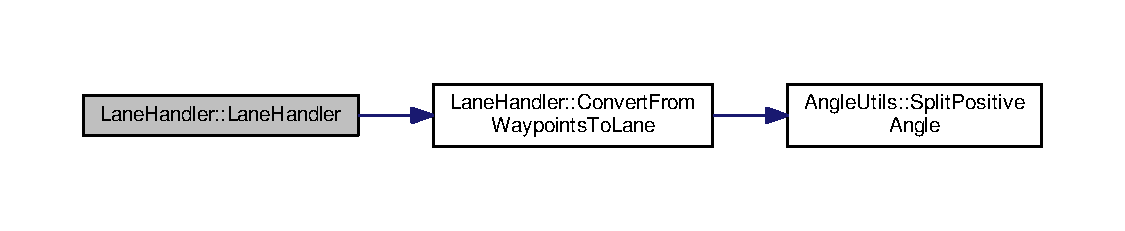
\includegraphics[width=350pt]{class_lane_handler_af9236889af0e7d75ca3230d47175a9b5_cgraph}
\end{center}
\end{figure}


\index{Lane\+Handler@{Lane\+Handler}!Lane\+Handler@{Lane\+Handler}}
\index{Lane\+Handler@{Lane\+Handler}!Lane\+Handler@{Lane\+Handler}}
\subsubsection[{\texorpdfstring{Lane\+Handler(const autoware\+\_\+msgs\+::lane \&lane)}{LaneHandler(const autoware_msgs::lane &lane)}}]{\setlength{\rightskip}{0pt plus 5cm}Lane\+Handler\+::\+Lane\+Handler (
\begin{DoxyParamCaption}
\item[{const autoware\+\_\+msgs\+::lane \&}]{lane}
\end{DoxyParamCaption}
)}\hypertarget{class_lane_handler_af00842c287a4ea45b48a0d928b861048}{}\label{class_lane_handler_af00842c287a4ea45b48a0d928b861048}


lane\+\_\+handler.\+cpp 파일의 18 번째 라인에서 정의되었습니다.


\begin{DoxyCode}
19 \{
20   \hyperlink{class_lane_handler_a167378a780eafb8242f7b12bd5460ac0}{autoware\_lane\_} = lane;
21   \hyperlink{class_lane_handler_a48d47e25edd09df1aa859904bd68c8f1}{convertFromLaneToWaypoints}(lane, \hyperlink{class_lane_handler_ac65a0139b3900a7c8dc3fe49d7a684f3}{waypoints\_lane\_});
22 \}
\end{DoxyCode}


이 함수 내부에서 호출하는 함수들에 대한 그래프입니다.\+:\nopagebreak
\begin{figure}[H]
\begin{center}
\leavevmode
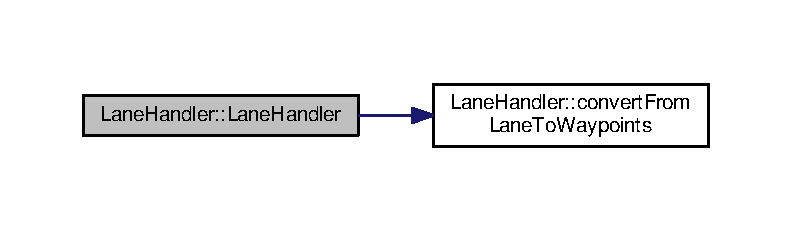
\includegraphics[width=350pt]{class_lane_handler_af00842c287a4ea45b48a0d928b861048_cgraph}
\end{center}
\end{figure}




\subsection{멤버 함수 문서화}
\index{Lane\+Handler@{Lane\+Handler}!convert\+From\+Lane\+To\+Waypoints@{convert\+From\+Lane\+To\+Waypoints}}
\index{convert\+From\+Lane\+To\+Waypoints@{convert\+From\+Lane\+To\+Waypoints}!Lane\+Handler@{Lane\+Handler}}
\subsubsection[{\texorpdfstring{convert\+From\+Lane\+To\+Waypoints(const autoware\+\_\+msgs\+::lane \&lane, std\+::vector$<$ Way\+Point $>$ \&path)}{convertFromLaneToWaypoints(const autoware_msgs::lane &lane, std::vector< WayPoint > &path)}}]{\setlength{\rightskip}{0pt plus 5cm}void Lane\+Handler\+::convert\+From\+Lane\+To\+Waypoints (
\begin{DoxyParamCaption}
\item[{const autoware\+\_\+msgs\+::lane \&}]{lane, }
\item[{std\+::vector$<$ {\bf Way\+Point} $>$ \&}]{path}
\end{DoxyParamCaption}
)\hspace{0.3cm}{\ttfamily [protected]}}\hypertarget{class_lane_handler_a48d47e25edd09df1aa859904bd68c8f1}{}\label{class_lane_handler_a48d47e25edd09df1aa859904bd68c8f1}


lane\+\_\+handler.\+cpp 파일의 42 번째 라인에서 정의되었습니다.


\begin{DoxyCode}
43 \{
44   \textcolor{keywordflow}{for}(\textcolor{keywordtype}{unsigned} \textcolor{keywordtype}{int} j = 0 ; j < lane.waypoints.size(); j++)
45   \{
46     \hyperlink{class_way_point}{WayPoint} wp(lane.waypoints.at(j).pose.pose.position.x,
47                 lane.waypoints.at(j).pose.pose.position.y,
48                 lane.waypoints.at(j).pose.pose.position.z,
49                 tf::getYaw(lane.waypoints.at(j).pose.pose.orientation));
50     wp.v\_ = lane.waypoints.at(j).twist.twist.linear.x;
51     path.push\_back(wp);
52   \}
53 \}
\end{DoxyCode}


이 함수를 호출하는 함수들에 대한 그래프입니다.\+:\nopagebreak
\begin{figure}[H]
\begin{center}
\leavevmode
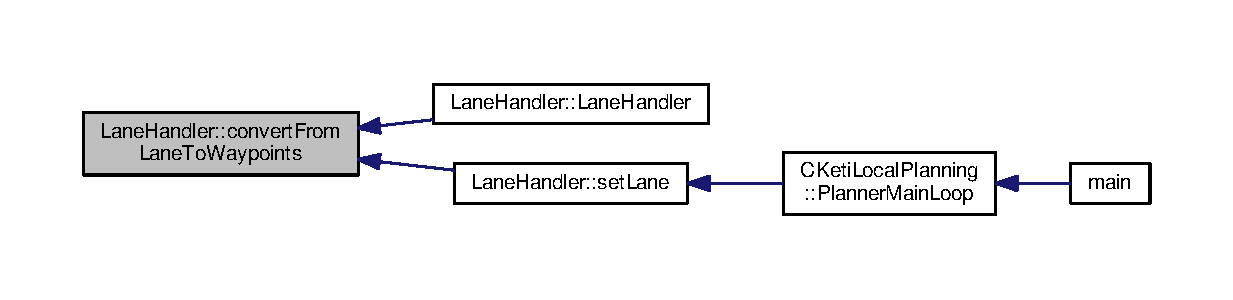
\includegraphics[width=350pt]{class_lane_handler_a48d47e25edd09df1aa859904bd68c8f1_icgraph}
\end{center}
\end{figure}


\index{Lane\+Handler@{Lane\+Handler}!Convert\+From\+Waypoints\+To\+Lane@{Convert\+From\+Waypoints\+To\+Lane}}
\index{Convert\+From\+Waypoints\+To\+Lane@{Convert\+From\+Waypoints\+To\+Lane}!Lane\+Handler@{Lane\+Handler}}
\subsubsection[{\texorpdfstring{Convert\+From\+Waypoints\+To\+Lane(const std\+::vector$<$ Way\+Point $>$ \&path, const int \&i\+Start, autoware\+\_\+msgs\+::lane \&trajectory)}{ConvertFromWaypointsToLane(const std::vector< WayPoint > &path, const int &iStart, autoware_msgs::lane &trajectory)}}]{\setlength{\rightskip}{0pt plus 5cm}void Lane\+Handler\+::\+Convert\+From\+Waypoints\+To\+Lane (
\begin{DoxyParamCaption}
\item[{const std\+::vector$<$ {\bf Way\+Point} $>$ \&}]{path, }
\item[{const int \&}]{i\+Start, }
\item[{autoware\+\_\+msgs\+::lane \&}]{trajectory}
\end{DoxyParamCaption}
)\hspace{0.3cm}{\ttfamily [protected]}}\hypertarget{class_lane_handler_a70a120b84428226b70754055b42dca2f}{}\label{class_lane_handler_a70a120b84428226b70754055b42dca2f}


lane\+\_\+handler.\+cpp 파일의 55 번째 라인에서 정의되었습니다.


\begin{DoxyCode}
57 \{
58   trajectory.waypoints.clear();
59   \textcolor{keywordflow}{for}(\textcolor{keywordtype}{unsigned} \textcolor{keywordtype}{int} i=iStart; i < path.size(); i++)
60   \{
61     autoware\_msgs::waypoint wp;
62     wp.pose.pose.position.x = path.at(i).pos\_.x\_;
63     wp.pose.pose.position.y = path.at(i).pos\_.y\_;
64     wp.pose.pose.position.z = path.at(i).pos\_.z\_;
65     wp.pose.pose.orientation = tf::createQuaternionMsgFromYaw(
      \hyperlink{class_angle_utils_a91f3e34c9e1e35788d44a2f6bc5bc206}{AngleUtils::SplitPositiveAngle}(path.at(i).pos\_.a\_));
66     wp.twist.twist.linear.x = path.at(i).v\_;
67     trajectory.waypoints.push\_back(wp);
68   \}
69 \}
\end{DoxyCode}


이 함수 내부에서 호출하는 함수들에 대한 그래프입니다.\+:\nopagebreak
\begin{figure}[H]
\begin{center}
\leavevmode
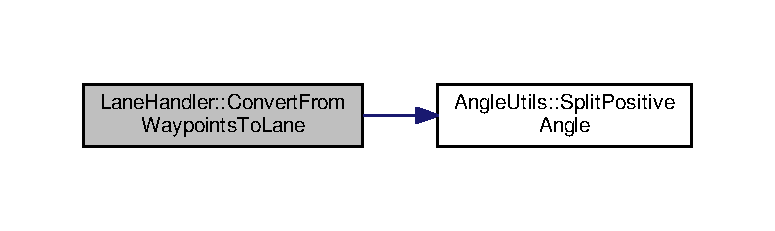
\includegraphics[width=350pt]{class_lane_handler_a70a120b84428226b70754055b42dca2f_cgraph}
\end{center}
\end{figure}




이 함수를 호출하는 함수들에 대한 그래프입니다.\+:\nopagebreak
\begin{figure}[H]
\begin{center}
\leavevmode
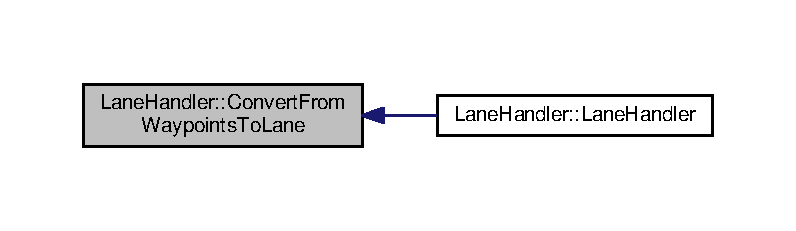
\includegraphics[width=350pt]{class_lane_handler_a70a120b84428226b70754055b42dca2f_icgraph}
\end{center}
\end{figure}


\index{Lane\+Handler@{Lane\+Handler}!get\+Autoware\+Lane@{get\+Autoware\+Lane}}
\index{get\+Autoware\+Lane@{get\+Autoware\+Lane}!Lane\+Handler@{Lane\+Handler}}
\subsubsection[{\texorpdfstring{get\+Autoware\+Lane()}{getAutowareLane()}}]{\setlength{\rightskip}{0pt plus 5cm}autoware\+\_\+msgs\+::lane Lane\+Handler\+::get\+Autoware\+Lane (
\begin{DoxyParamCaption}
{}
\end{DoxyParamCaption}
)}\hypertarget{class_lane_handler_a9d66775c597130ccbd369d50c7572c2e}{}\label{class_lane_handler_a9d66775c597130ccbd369d50c7572c2e}


lane\+\_\+handler.\+cpp 파일의 33 번째 라인에서 정의되었습니다.


\begin{DoxyCode}
34 \{
35   \textcolor{keywordflow}{return} \hyperlink{class_lane_handler_a167378a780eafb8242f7b12bd5460ac0}{autoware\_lane\_};
36 \}
\end{DoxyCode}


이 함수를 호출하는 함수들에 대한 그래프입니다.\+:\nopagebreak
\begin{figure}[H]
\begin{center}
\leavevmode
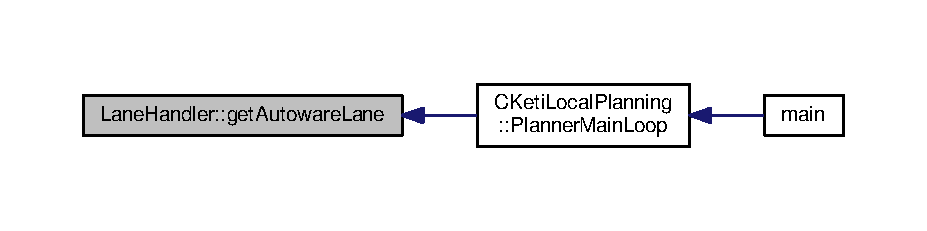
\includegraphics[width=350pt]{class_lane_handler_a9d66775c597130ccbd369d50c7572c2e_icgraph}
\end{center}
\end{figure}


\index{Lane\+Handler@{Lane\+Handler}!get\+Closest\+Waypoint@{get\+Closest\+Waypoint}}
\index{get\+Closest\+Waypoint@{get\+Closest\+Waypoint}!Lane\+Handler@{Lane\+Handler}}
\subsubsection[{\texorpdfstring{get\+Closest\+Waypoint(const geometry\+\_\+msgs\+::\+Pose \&wp)}{getClosestWaypoint(const geometry_msgs::Pose &wp)}}]{\setlength{\rightskip}{0pt plus 5cm}int Lane\+Handler\+::get\+Closest\+Waypoint (
\begin{DoxyParamCaption}
\item[{const geometry\+\_\+msgs\+::\+Pose \&}]{current\+\_\+pose}
\end{DoxyParamCaption}
)}\hypertarget{class_lane_handler_a71033c4e67c07e09c2c3c18fabfb7463}{}\label{class_lane_handler_a71033c4e67c07e09c2c3c18fabfb7463}


Find a point on the lane which is the closest point to the \hyperlink{class_way_point}{Way\+Point}. 

Find the closest waypoint index on the lane from point.


\begin{DoxyParams}{매개변수}
{\em wp} & \\
\hline
\end{DoxyParams}
\begin{DoxyReturn}{반환값}
index of the closest waypoint on the lane.
\end{DoxyReturn}

\begin{DoxyParams}{매개변수}
{\em current\+\_\+pose} & \\
\hline
\end{DoxyParams}
\begin{DoxyReturn}{반환값}

\end{DoxyReturn}


lane\+\_\+handler.\+cpp 파일의 77 번째 라인에서 정의되었습니다.


\begin{DoxyCode}
78 \{
79 
80   \textcolor{keywordflow}{if} (\hyperlink{class_lane_handler_ac65a0139b3900a7c8dc3fe49d7a684f3}{waypoints\_lane\_}.empty()==\textcolor{keyword}{true})
81     \textcolor{keywordflow}{return} -1;
82 
83   \textcolor{comment}{// search closest candidate within a certain meter}
84   \textcolor{keywordtype}{double} search\_distance = 5.0;
85   std::vector<int> waypoint\_candidates;
86   \hyperlink{class_pose_point_handler}{PosePointHandler} pp\_handler;
87 
88   \textcolor{keywordflow}{for} (\textcolor{keywordtype}{unsigned} \textcolor{keywordtype}{int} i = 1; i < \hyperlink{class_lane_handler_ac65a0139b3900a7c8dc3fe49d7a684f3}{waypoints\_lane\_}.size(); i++)
89   \{
90     pp\_handler.\hyperlink{class_pose_point_handler_a6d037671a1c93d9d51a7b0e40eacd3fa}{setPosePoint}(current\_pose,\hyperlink{class_lane_handler_ac65a0139b3900a7c8dc3fe49d7a684f3}{waypoints\_lane\_}.at(i).getPoint());
91     \textcolor{keywordflow}{if} (\hyperlink{class_lane_handler_ac65a0139b3900a7c8dc3fe49d7a684f3}{waypoints\_lane\_}.at(i).getDistance(current\_pose.position) > search\_distance)
92       \textcolor{keywordflow}{continue};
93 
94     \textcolor{keywordflow}{if} (!pp\_handler.\hyperlink{class_pose_point_handler_a030d4318ea42d398798b675624ebd07b}{isPoisitionInFrontOfPose}())
95       \textcolor{keywordflow}{continue};
96 
97     waypoint\_candidates.push\_back(i);
98   \}
99 
100   \textcolor{comment}{// get closest waypoint from candidates}
101   \textcolor{keywordflow}{if} (!waypoint\_candidates.empty())
102   \{
103     \textcolor{keywordtype}{int} waypoint\_min = -1;
104     \textcolor{keywordtype}{double} distance\_min = DBL\_MAX;
105     \textcolor{keywordflow}{for}(uint el=0; el<waypoint\_candidates.size();el++)
106     \{
107       \textcolor{keywordtype}{int} cur\_way = waypoint\_candidates.at(el);
108       \textcolor{keywordtype}{double} d = \hyperlink{class_lane_handler_ac65a0139b3900a7c8dc3fe49d7a684f3}{waypoints\_lane\_}.at(cur\_way).getDistance(current\_pose.position);
109       \textcolor{keywordflow}{if} (d < distance\_min)
110       \{
111         waypoint\_min = cur\_way;
112         distance\_min = d;
113       \}
114     \}
115     \textcolor{keywordflow}{return} waypoint\_min;
116   \}
117   \textcolor{keywordflow}{else}
118   \{
119     ROS\_INFO(\textcolor{stringliteral}{"no candidate. search closest waypoint from all waypoints..."});
120     \textcolor{comment}{// if there is no candidate...}
121     \textcolor{keywordtype}{int} waypoint\_min = -1;
122     \textcolor{keywordtype}{double} distance\_min = DBL\_MAX;
123     \textcolor{keywordflow}{for} (\textcolor{keywordtype}{unsigned} \textcolor{keywordtype}{int} i = 1; i <\hyperlink{class_lane_handler_ac65a0139b3900a7c8dc3fe49d7a684f3}{waypoints\_lane\_}.size(); i++)
124     \{
125       pp\_handler.\hyperlink{class_pose_point_handler_a6d037671a1c93d9d51a7b0e40eacd3fa}{setPosePoint}(current\_pose,\hyperlink{class_lane_handler_ac65a0139b3900a7c8dc3fe49d7a684f3}{waypoints\_lane\_}.at(i).getPoint());
126 
127       \textcolor{keywordflow}{if} (!pp\_handler.\hyperlink{class_pose_point_handler_a030d4318ea42d398798b675624ebd07b}{isPoisitionInFrontOfPose}())
128         \textcolor{keywordflow}{continue};
129 
130 
131       \textcolor{keywordtype}{double} d = \hyperlink{class_lane_handler_ac65a0139b3900a7c8dc3fe49d7a684f3}{waypoints\_lane\_}.at(i).getDistance(current\_pose.position);
132       \textcolor{keywordflow}{if} (d < distance\_min)
133       \{
134         waypoint\_min = i;
135         distance\_min = d;
136       \}
137     \}
138     \textcolor{keywordflow}{return} waypoint\_min;
139   \}
140 \}
\end{DoxyCode}


이 함수 내부에서 호출하는 함수들에 대한 그래프입니다.\+:\nopagebreak
\begin{figure}[H]
\begin{center}
\leavevmode
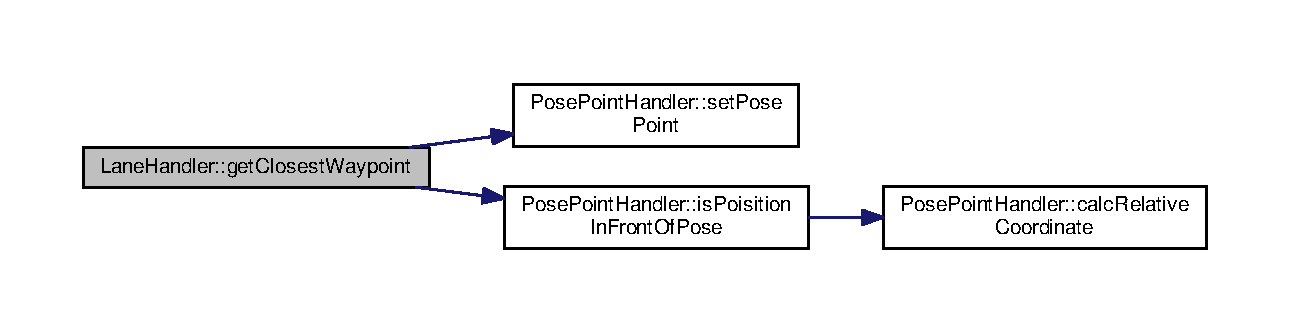
\includegraphics[width=350pt]{class_lane_handler_a71033c4e67c07e09c2c3c18fabfb7463_cgraph}
\end{center}
\end{figure}




이 함수를 호출하는 함수들에 대한 그래프입니다.\+:\nopagebreak
\begin{figure}[H]
\begin{center}
\leavevmode
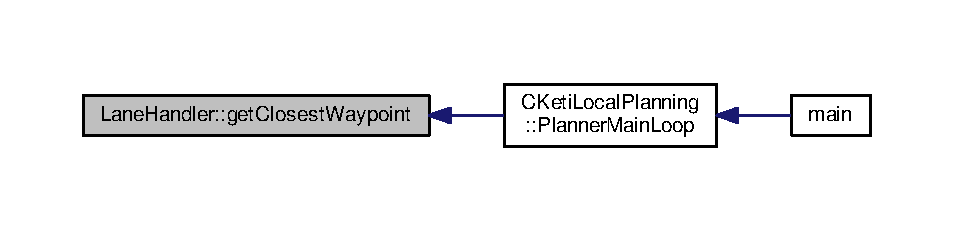
\includegraphics[width=350pt]{class_lane_handler_a71033c4e67c07e09c2c3c18fabfb7463_icgraph}
\end{center}
\end{figure}


\index{Lane\+Handler@{Lane\+Handler}!get\+Waypoints\+Lane@{get\+Waypoints\+Lane}}
\index{get\+Waypoints\+Lane@{get\+Waypoints\+Lane}!Lane\+Handler@{Lane\+Handler}}
\subsubsection[{\texorpdfstring{get\+Waypoints\+Lane()}{getWaypointsLane()}}]{\setlength{\rightskip}{0pt plus 5cm}std\+::vector$<$ {\bf Way\+Point} $>$ Lane\+Handler\+::get\+Waypoints\+Lane (
\begin{DoxyParamCaption}
{}
\end{DoxyParamCaption}
)}\hypertarget{class_lane_handler_afe241272b5017d7d0e439d08bbf855d9}{}\label{class_lane_handler_afe241272b5017d7d0e439d08bbf855d9}


lane\+\_\+handler.\+cpp 파일의 37 번째 라인에서 정의되었습니다.


\begin{DoxyCode}
38 \{
39   \textcolor{keywordflow}{return} \hyperlink{class_lane_handler_ac65a0139b3900a7c8dc3fe49d7a684f3}{waypoints\_lane\_};
40 \}
\end{DoxyCode}
\index{Lane\+Handler@{Lane\+Handler}!set\+Lane@{set\+Lane}}
\index{set\+Lane@{set\+Lane}!Lane\+Handler@{Lane\+Handler}}
\subsubsection[{\texorpdfstring{set\+Lane(const autoware\+\_\+msgs\+::lane \&lane)}{setLane(const autoware_msgs::lane &lane)}}]{\setlength{\rightskip}{0pt plus 5cm}void Lane\+Handler\+::set\+Lane (
\begin{DoxyParamCaption}
\item[{const autoware\+\_\+msgs\+::lane \&}]{lane}
\end{DoxyParamCaption}
)}\hypertarget{class_lane_handler_a6c4cc7f5ae19a81cd24ba1427b0afb74}{}\label{class_lane_handler_a6c4cc7f5ae19a81cd24ba1427b0afb74}


lane\+\_\+handler.\+cpp 파일의 23 번째 라인에서 정의되었습니다.


\begin{DoxyCode}
24 \{
25   \hyperlink{class_lane_handler_a167378a780eafb8242f7b12bd5460ac0}{autoware\_lane\_} = lane;
26   \hyperlink{class_lane_handler_a48d47e25edd09df1aa859904bd68c8f1}{convertFromLaneToWaypoints}(lane, \hyperlink{class_lane_handler_ac65a0139b3900a7c8dc3fe49d7a684f3}{waypoints\_lane\_});
27 \}
\end{DoxyCode}


이 함수 내부에서 호출하는 함수들에 대한 그래프입니다.\+:\nopagebreak
\begin{figure}[H]
\begin{center}
\leavevmode
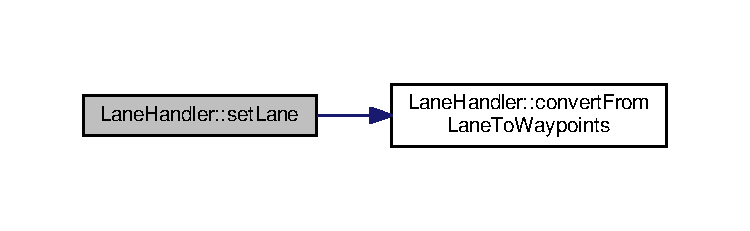
\includegraphics[width=350pt]{class_lane_handler_a6c4cc7f5ae19a81cd24ba1427b0afb74_cgraph}
\end{center}
\end{figure}




이 함수를 호출하는 함수들에 대한 그래프입니다.\+:\nopagebreak
\begin{figure}[H]
\begin{center}
\leavevmode
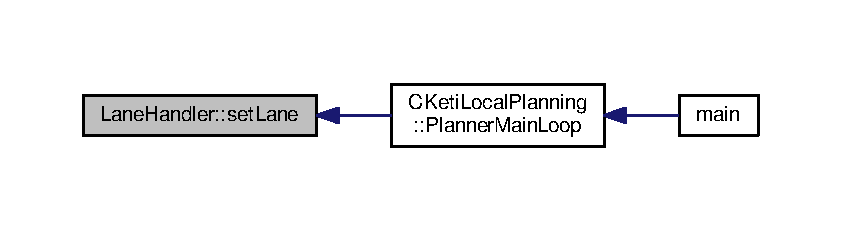
\includegraphics[width=350pt]{class_lane_handler_a6c4cc7f5ae19a81cd24ba1427b0afb74_icgraph}
\end{center}
\end{figure}


\index{Lane\+Handler@{Lane\+Handler}!set\+Lane@{set\+Lane}}
\index{set\+Lane@{set\+Lane}!Lane\+Handler@{Lane\+Handler}}
\subsubsection[{\texorpdfstring{set\+Lane(const std\+::vector$<$ Way\+Point $>$ \&lane)}{setLane(const std::vector< WayPoint > &lane)}}]{\setlength{\rightskip}{0pt plus 5cm}void Lane\+Handler\+::set\+Lane (
\begin{DoxyParamCaption}
\item[{const std\+::vector$<$ {\bf Way\+Point} $>$ \&}]{lane}
\end{DoxyParamCaption}
)}\hypertarget{class_lane_handler_a33776b288c92ee7e63f865e6c9526ff3}{}\label{class_lane_handler_a33776b288c92ee7e63f865e6c9526ff3}


lane\+\_\+handler.\+cpp 파일의 28 번째 라인에서 정의되었습니다.


\begin{DoxyCode}
29 \{
30   \hyperlink{class_lane_handler_ac65a0139b3900a7c8dc3fe49d7a684f3}{waypoints\_lane\_} = lane;
31 \}
\end{DoxyCode}


\subsection{멤버 데이타 문서화}
\index{Lane\+Handler@{Lane\+Handler}!autoware\+\_\+lane\+\_\+@{autoware\+\_\+lane\+\_\+}}
\index{autoware\+\_\+lane\+\_\+@{autoware\+\_\+lane\+\_\+}!Lane\+Handler@{Lane\+Handler}}
\subsubsection[{\texorpdfstring{autoware\+\_\+lane\+\_\+}{autoware_lane_}}]{\setlength{\rightskip}{0pt plus 5cm}autoware\+\_\+msgs\+::lane Lane\+Handler\+::autoware\+\_\+lane\+\_\+}\hypertarget{class_lane_handler_a167378a780eafb8242f7b12bd5460ac0}{}\label{class_lane_handler_a167378a780eafb8242f7b12bd5460ac0}


lane\+\_\+handler.\+h 파일의 17 번째 라인에서 정의되었습니다.

\index{Lane\+Handler@{Lane\+Handler}!waypoints\+\_\+lane\+\_\+@{waypoints\+\_\+lane\+\_\+}}
\index{waypoints\+\_\+lane\+\_\+@{waypoints\+\_\+lane\+\_\+}!Lane\+Handler@{Lane\+Handler}}
\subsubsection[{\texorpdfstring{waypoints\+\_\+lane\+\_\+}{waypoints_lane_}}]{\setlength{\rightskip}{0pt plus 5cm}std\+::vector$<${\bf Way\+Point}$>$ Lane\+Handler\+::waypoints\+\_\+lane\+\_\+}\hypertarget{class_lane_handler_ac65a0139b3900a7c8dc3fe49d7a684f3}{}\label{class_lane_handler_ac65a0139b3900a7c8dc3fe49d7a684f3}


lane\+\_\+handler.\+h 파일의 16 번째 라인에서 정의되었습니다.



이 클래스에 대한 문서화 페이지는 다음의 파일들로부터 생성되었습니다.\+:\begin{DoxyCompactItemize}
\item 
/home/dallddungi/keti\+\_\+ws/src/keti\+\_\+local\+\_\+planning/include/data\+\_\+handler/\hyperlink{lane__handler_8h}{lane\+\_\+handler.\+h}\item 
/home/dallddungi/keti\+\_\+ws/src/keti\+\_\+local\+\_\+planning/src/data\+\_\+handler/\hyperlink{lane__handler_8cpp}{lane\+\_\+handler.\+cpp}\end{DoxyCompactItemize}

\hypertarget{class_point_handler}{}\section{Point\+Handler 클래스 참조}
\label{class_point_handler}\index{Point\+Handler@{Point\+Handler}}


Point handling class.  




{\ttfamily \#include $<$point\+\_\+handler.\+h$>$}



Point\+Handler에 대한 협력 다이어그램\+:\nopagebreak
\begin{figure}[H]
\begin{center}
\leavevmode
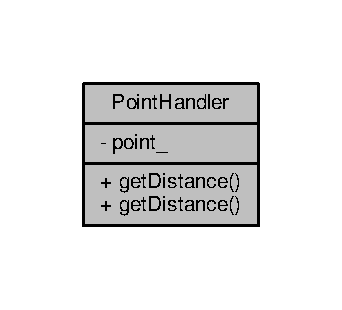
\includegraphics[width=164pt]{class_point_handler__coll__graph}
\end{center}
\end{figure}
\subsection*{Public 멤버 함수}
\begin{DoxyCompactItemize}
\item 
double \hyperlink{class_point_handler_ae5d42991d2fe2a2e89afc4defc9158e1}{get\+Distance} (geometry\+\_\+msgs\+::\+Point point)
\item 
double \hyperlink{class_point_handler_ae5d42991d2fe2a2e89afc4defc9158e1}{get\+Distance} (geometry\+\_\+msgs\+::\+Point point)
\end{DoxyCompactItemize}
\subsection*{Private 속성}
\begin{DoxyCompactItemize}
\item 
geometry\+\_\+msgs\+::\+Point \hyperlink{class_point_handler_ad95d3d370852a0dfb97f099e01934f6a}{point\+\_\+}
\end{DoxyCompactItemize}


\subsection{상세한 설명}
Point handling class. 

point\+\_\+handler.\+h 파일의 11 번째 라인에서 정의되었습니다.



\subsection{멤버 함수 문서화}
\index{Point\+Handler@{Point\+Handler}!get\+Distance@{get\+Distance}}
\index{get\+Distance@{get\+Distance}!Point\+Handler@{Point\+Handler}}
\subsubsection[{\texorpdfstring{get\+Distance(geometry\+\_\+msgs\+::\+Point point)}{getDistance(geometry_msgs::Point point)}}]{\setlength{\rightskip}{0pt plus 5cm}double Point\+Handler\+::get\+Distance (
\begin{DoxyParamCaption}
\item[{geometry\+\_\+msgs\+::\+Point}]{point}
\end{DoxyParamCaption}
)\hspace{0.3cm}{\ttfamily [inline]}}\hypertarget{class_point_handler_ae5d42991d2fe2a2e89afc4defc9158e1}{}\label{class_point_handler_ae5d42991d2fe2a2e89afc4defc9158e1}


point\+\_\+handler.\+h 파일의 15 번째 라인에서 정의되었습니다.


\begin{DoxyCode}
16   \{
17     \textcolor{keywordflow}{return} sqrt(pow(point.x-\hyperlink{class_point_handler_ad95d3d370852a0dfb97f099e01934f6a}{point\_}.x,2)+pow(point.y-\hyperlink{class_point_handler_ad95d3d370852a0dfb97f099e01934f6a}{point\_}.y,2)+pow(point.z-
      \hyperlink{class_point_handler_ad95d3d370852a0dfb97f099e01934f6a}{point\_}.z,2));
18   \}
\end{DoxyCode}
\index{Point\+Handler@{Point\+Handler}!get\+Distance@{get\+Distance}}
\index{get\+Distance@{get\+Distance}!Point\+Handler@{Point\+Handler}}
\subsubsection[{\texorpdfstring{get\+Distance(geometry\+\_\+msgs\+::\+Point point)}{getDistance(geometry_msgs::Point point)}}]{\setlength{\rightskip}{0pt plus 5cm}double Point\+Handler\+::get\+Distance (
\begin{DoxyParamCaption}
\item[{geometry\+\_\+msgs\+::\+Point}]{point}
\end{DoxyParamCaption}
)\hspace{0.3cm}{\ttfamily [inline]}}\hypertarget{class_point_handler_ae5d42991d2fe2a2e89afc4defc9158e1}{}\label{class_point_handler_ae5d42991d2fe2a2e89afc4defc9158e1}


point\+\_\+handler.\+h 파일의 15 번째 라인에서 정의되었습니다.


\begin{DoxyCode}
16   \{
17     \textcolor{keywordflow}{return} sqrt(pow(point.x-\hyperlink{class_point_handler_ad95d3d370852a0dfb97f099e01934f6a}{point\_}.x,2)+pow(point.y-\hyperlink{class_point_handler_ad95d3d370852a0dfb97f099e01934f6a}{point\_}.y,2)+pow(point.z-
      \hyperlink{class_point_handler_ad95d3d370852a0dfb97f099e01934f6a}{point\_}.z,2));
18   \}
\end{DoxyCode}


\subsection{멤버 데이타 문서화}
\index{Point\+Handler@{Point\+Handler}!point\+\_\+@{point\+\_\+}}
\index{point\+\_\+@{point\+\_\+}!Point\+Handler@{Point\+Handler}}
\subsubsection[{\texorpdfstring{point\+\_\+}{point_}}]{\setlength{\rightskip}{0pt plus 5cm}geometry\+\_\+msgs\+::\+Point Point\+Handler\+::point\+\_\+\hspace{0.3cm}{\ttfamily [private]}}\hypertarget{class_point_handler_ad95d3d370852a0dfb97f099e01934f6a}{}\label{class_point_handler_ad95d3d370852a0dfb97f099e01934f6a}


point\+\_\+handler.\+h 파일의 13 번째 라인에서 정의되었습니다.



이 클래스에 대한 문서화 페이지는 다음의 파일로부터 생성되었습니다.\+:\begin{DoxyCompactItemize}
\item 
/home/dallddungi/keti\+\_\+ws/src/keti\+\_\+local\+\_\+planning/include/data\+\_\+handler/\hyperlink{point__handler_8h}{point\+\_\+handler.\+h}\end{DoxyCompactItemize}

\hypertarget{class_pose_point_handler}{}\section{Pose\+Point\+Handler 클래스 참조}
\label{class_pose_point_handler}\index{Pose\+Point\+Handler@{Pose\+Point\+Handler}}


The Pose\+Position\+Handler class.  




{\ttfamily \#include $<$pose\+\_\+point\+\_\+handler.\+h$>$}



Pose\+Point\+Handler에 대한 협력 다이어그램\+:\nopagebreak
\begin{figure}[H]
\begin{center}
\leavevmode
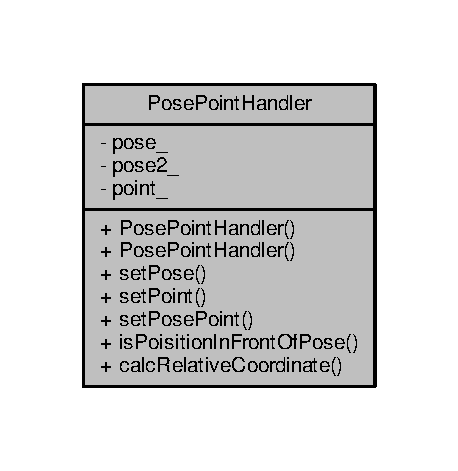
\includegraphics[width=220pt]{class_pose_point_handler__coll__graph}
\end{center}
\end{figure}
\subsection*{Public 멤버 함수}
\begin{DoxyCompactItemize}
\item 
\hyperlink{class_pose_point_handler_a752ad3fb30dbe034908e7e6be50b9a42}{Pose\+Point\+Handler} ()
\item 
\hyperlink{class_pose_point_handler_a6c9b665fb0434622641bb1c1e71d40ef}{Pose\+Point\+Handler} (const geometry\+\_\+msgs\+::\+Pose \&pose, const geometry\+\_\+msgs\+::\+Point \&point)
\item 
void \hyperlink{class_pose_point_handler_ae75fcd9ec5c7dcf9194939aa631e47ae}{set\+Pose} (const geometry\+\_\+msgs\+::\+Pose \&pose)
\item 
void \hyperlink{class_pose_point_handler_a948561235698288597b3c65f03f1d1aa}{set\+Point} (const geometry\+\_\+msgs\+::\+Point \&point)
\item 
void \hyperlink{class_pose_point_handler_a6d037671a1c93d9d51a7b0e40eacd3fa}{set\+Pose\+Point} (const geometry\+\_\+msgs\+::\+Pose \&pose, const geometry\+\_\+msgs\+::\+Point \&point)
\item 
bool \hyperlink{class_pose_point_handler_a030d4318ea42d398798b675624ebd07b}{is\+Poisition\+In\+Front\+Of\+Pose} ()
\begin{DoxyCompactList}\small\item\em Check whether a point is in the front of the current\+\_\+pose. \end{DoxyCompactList}\item 
geometry\+\_\+msgs\+::\+Point \hyperlink{class_pose_point_handler_a8ca33b37d5cb22e1310b863fcb94676c}{calc\+Relative\+Coordinate} ()
\end{DoxyCompactItemize}
\subsection*{Private 속성}
\begin{DoxyCompactItemize}
\item 
geometry\+\_\+msgs\+::\+Pose \hyperlink{class_pose_point_handler_ab78a62b6b03dee10487bf53339685a7d}{pose\+\_\+}
\item 
geometry\+\_\+msgs\+::\+Pose \hyperlink{class_pose_point_handler_ad615a2da1c3cd5cc3b5162390dac6136}{pose2\+\_\+}
\item 
geometry\+\_\+msgs\+::\+Point \hyperlink{class_pose_point_handler_aa6dc915c1a9a98a64dd78c51f4b5ae02}{point\+\_\+}
\end{DoxyCompactItemize}


\subsection{상세한 설명}
The Pose\+Position\+Handler class. 

pose\+\_\+point\+\_\+handler.\+h 파일의 10 번째 라인에서 정의되었습니다.



\subsection{생성자 \& 소멸자 문서화}
\index{Pose\+Point\+Handler@{Pose\+Point\+Handler}!Pose\+Point\+Handler@{Pose\+Point\+Handler}}
\index{Pose\+Point\+Handler@{Pose\+Point\+Handler}!Pose\+Point\+Handler@{Pose\+Point\+Handler}}
\subsubsection[{\texorpdfstring{Pose\+Point\+Handler()}{PosePointHandler()}}]{\setlength{\rightskip}{0pt plus 5cm}Pose\+Point\+Handler\+::\+Pose\+Point\+Handler (
\begin{DoxyParamCaption}
{}
\end{DoxyParamCaption}
)}\hypertarget{class_pose_point_handler_a752ad3fb30dbe034908e7e6be50b9a42}{}\label{class_pose_point_handler_a752ad3fb30dbe034908e7e6be50b9a42}


pose\+\_\+point\+\_\+handler.\+cpp 파일의 4 번째 라인에서 정의되었습니다.


\begin{DoxyCode}
5 \{
6 
7 \}
\end{DoxyCode}
\index{Pose\+Point\+Handler@{Pose\+Point\+Handler}!Pose\+Point\+Handler@{Pose\+Point\+Handler}}
\index{Pose\+Point\+Handler@{Pose\+Point\+Handler}!Pose\+Point\+Handler@{Pose\+Point\+Handler}}
\subsubsection[{\texorpdfstring{Pose\+Point\+Handler(const geometry\+\_\+msgs\+::\+Pose \&pose, const geometry\+\_\+msgs\+::\+Point \&point)}{PosePointHandler(const geometry_msgs::Pose &pose, const geometry_msgs::Point &point)}}]{\setlength{\rightskip}{0pt plus 5cm}Pose\+Point\+Handler\+::\+Pose\+Point\+Handler (
\begin{DoxyParamCaption}
\item[{const geometry\+\_\+msgs\+::\+Pose \&}]{pose, }
\item[{const geometry\+\_\+msgs\+::\+Point \&}]{point}
\end{DoxyParamCaption}
)}\hypertarget{class_pose_point_handler_a6c9b665fb0434622641bb1c1e71d40ef}{}\label{class_pose_point_handler_a6c9b665fb0434622641bb1c1e71d40ef}


pose\+\_\+point\+\_\+handler.\+cpp 파일의 8 번째 라인에서 정의되었습니다.


\begin{DoxyCode}
9 \{
10   \hyperlink{class_pose_point_handler_ab78a62b6b03dee10487bf53339685a7d}{pose\_} = pose;
11   \hyperlink{class_pose_point_handler_aa6dc915c1a9a98a64dd78c51f4b5ae02}{point\_} = point;
12 \}
\end{DoxyCode}


\subsection{멤버 함수 문서화}
\index{Pose\+Point\+Handler@{Pose\+Point\+Handler}!calc\+Relative\+Coordinate@{calc\+Relative\+Coordinate}}
\index{calc\+Relative\+Coordinate@{calc\+Relative\+Coordinate}!Pose\+Point\+Handler@{Pose\+Point\+Handler}}
\subsubsection[{\texorpdfstring{calc\+Relative\+Coordinate()}{calcRelativeCoordinate()}}]{\setlength{\rightskip}{0pt plus 5cm}geometry\+\_\+msgs\+::\+Point Pose\+Point\+Handler\+::calc\+Relative\+Coordinate (
\begin{DoxyParamCaption}
{}
\end{DoxyParamCaption}
)}\hypertarget{class_pose_point_handler_a8ca33b37d5cb22e1310b863fcb94676c}{}\label{class_pose_point_handler_a8ca33b37d5cb22e1310b863fcb94676c}


pose\+\_\+point\+\_\+handler.\+cpp 파일의 36 번째 라인에서 정의되었습니다.


\begin{DoxyCode}
37 \{
38   tf::Transform inverse;
39   tf::poseMsgToTF(\hyperlink{class_pose_point_handler_ab78a62b6b03dee10487bf53339685a7d}{pose\_}, inverse);
40   tf::Transform transform = inverse.inverse();
41 
42   tf::Point p;
43   pointMsgToTF(\hyperlink{class_pose_point_handler_aa6dc915c1a9a98a64dd78c51f4b5ae02}{point\_}, p);
44   tf::Point tf\_p = transform * p;
45   geometry\_msgs::Point tf\_point\_msg;
46   pointTFToMsg(tf\_p, tf\_point\_msg);
47 
48   \textcolor{keywordflow}{return} tf\_point\_msg;
49 \}
\end{DoxyCode}


이 함수를 호출하는 함수들에 대한 그래프입니다.\+:\nopagebreak
\begin{figure}[H]
\begin{center}
\leavevmode
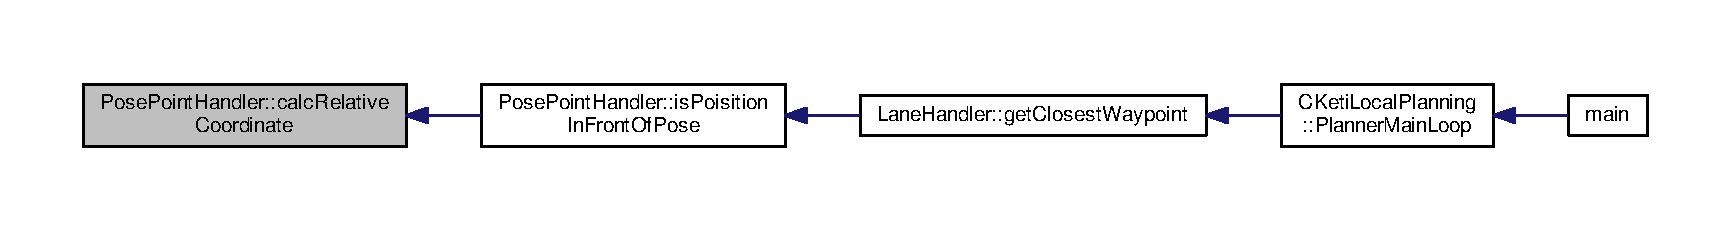
\includegraphics[width=350pt]{class_pose_point_handler_a8ca33b37d5cb22e1310b863fcb94676c_icgraph}
\end{center}
\end{figure}


\index{Pose\+Point\+Handler@{Pose\+Point\+Handler}!is\+Poisition\+In\+Front\+Of\+Pose@{is\+Poisition\+In\+Front\+Of\+Pose}}
\index{is\+Poisition\+In\+Front\+Of\+Pose@{is\+Poisition\+In\+Front\+Of\+Pose}!Pose\+Point\+Handler@{Pose\+Point\+Handler}}
\subsubsection[{\texorpdfstring{is\+Poisition\+In\+Front\+Of\+Pose()}{isPoisitionInFrontOfPose()}}]{\setlength{\rightskip}{0pt plus 5cm}bool Pose\+Point\+Handler\+::is\+Poisition\+In\+Front\+Of\+Pose (
\begin{DoxyParamCaption}
{}
\end{DoxyParamCaption}
)}\hypertarget{class_pose_point_handler_a030d4318ea42d398798b675624ebd07b}{}\label{class_pose_point_handler_a030d4318ea42d398798b675624ebd07b}


Check whether a point is in the front of the current\+\_\+pose. 


\begin{DoxyParams}{매개변수}
{\em pose} & data \\
\hline
\end{DoxyParams}
\begin{DoxyReturn}{반환값}
If ture, \hyperlink{class_way_point}{Way\+Point} is in front of the current pose. 
\end{DoxyReturn}


pose\+\_\+point\+\_\+handler.\+cpp 파일의 27 번째 라인에서 정의되었습니다.


\begin{DoxyCode}
28 \{
29   \textcolor{keywordtype}{double} x = \hyperlink{class_pose_point_handler_a8ca33b37d5cb22e1310b863fcb94676c}{PosePointHandler::calcRelativeCoordinate}().x;
30   \textcolor{keywordflow}{if} (x < 0)
31     \textcolor{keywordflow}{return} \textcolor{keyword}{false};
32   \textcolor{keywordflow}{else}
33     \textcolor{keywordflow}{return} \textcolor{keyword}{true};
34 \}
\end{DoxyCode}


이 함수 내부에서 호출하는 함수들에 대한 그래프입니다.\+:\nopagebreak
\begin{figure}[H]
\begin{center}
\leavevmode
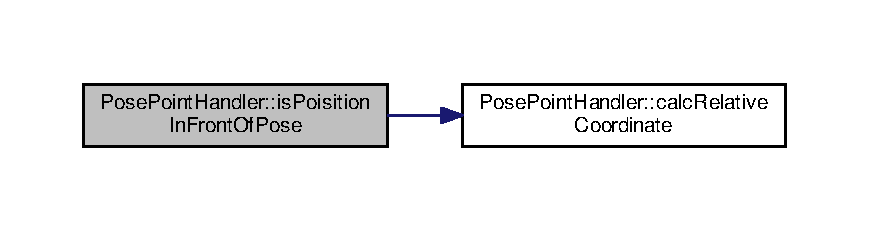
\includegraphics[width=350pt]{class_pose_point_handler_a030d4318ea42d398798b675624ebd07b_cgraph}
\end{center}
\end{figure}




이 함수를 호출하는 함수들에 대한 그래프입니다.\+:\nopagebreak
\begin{figure}[H]
\begin{center}
\leavevmode
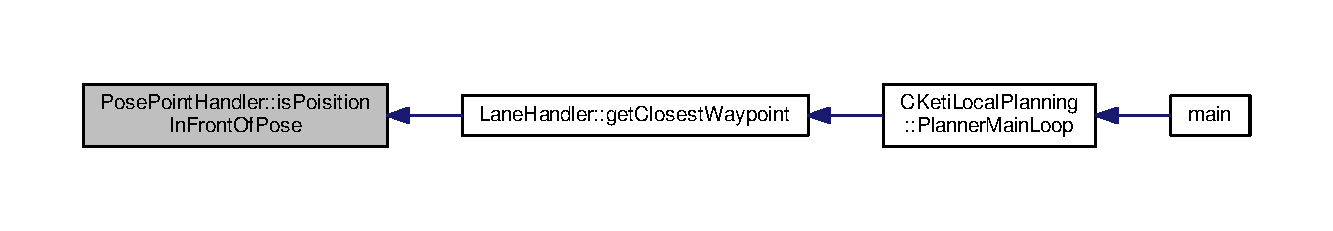
\includegraphics[width=350pt]{class_pose_point_handler_a030d4318ea42d398798b675624ebd07b_icgraph}
\end{center}
\end{figure}


\index{Pose\+Point\+Handler@{Pose\+Point\+Handler}!set\+Point@{set\+Point}}
\index{set\+Point@{set\+Point}!Pose\+Point\+Handler@{Pose\+Point\+Handler}}
\subsubsection[{\texorpdfstring{set\+Point(const geometry\+\_\+msgs\+::\+Point \&point)}{setPoint(const geometry_msgs::Point &point)}}]{\setlength{\rightskip}{0pt plus 5cm}void Pose\+Point\+Handler\+::set\+Point (
\begin{DoxyParamCaption}
\item[{const geometry\+\_\+msgs\+::\+Point \&}]{point}
\end{DoxyParamCaption}
)}\hypertarget{class_pose_point_handler_a948561235698288597b3c65f03f1d1aa}{}\label{class_pose_point_handler_a948561235698288597b3c65f03f1d1aa}


pose\+\_\+point\+\_\+handler.\+cpp 파일의 18 번째 라인에서 정의되었습니다.


\begin{DoxyCode}
19 \{
20   \hyperlink{class_pose_point_handler_aa6dc915c1a9a98a64dd78c51f4b5ae02}{point\_} = point;
21 \}
\end{DoxyCode}
\index{Pose\+Point\+Handler@{Pose\+Point\+Handler}!set\+Pose@{set\+Pose}}
\index{set\+Pose@{set\+Pose}!Pose\+Point\+Handler@{Pose\+Point\+Handler}}
\subsubsection[{\texorpdfstring{set\+Pose(const geometry\+\_\+msgs\+::\+Pose \&pose)}{setPose(const geometry_msgs::Pose &pose)}}]{\setlength{\rightskip}{0pt plus 5cm}void Pose\+Point\+Handler\+::set\+Pose (
\begin{DoxyParamCaption}
\item[{const geometry\+\_\+msgs\+::\+Pose \&}]{pose}
\end{DoxyParamCaption}
)}\hypertarget{class_pose_point_handler_ae75fcd9ec5c7dcf9194939aa631e47ae}{}\label{class_pose_point_handler_ae75fcd9ec5c7dcf9194939aa631e47ae}


pose\+\_\+point\+\_\+handler.\+cpp 파일의 14 번째 라인에서 정의되었습니다.


\begin{DoxyCode}
15 \{
16   \hyperlink{class_pose_point_handler_ab78a62b6b03dee10487bf53339685a7d}{pose\_} = pose;
17 \}
\end{DoxyCode}
\index{Pose\+Point\+Handler@{Pose\+Point\+Handler}!set\+Pose\+Point@{set\+Pose\+Point}}
\index{set\+Pose\+Point@{set\+Pose\+Point}!Pose\+Point\+Handler@{Pose\+Point\+Handler}}
\subsubsection[{\texorpdfstring{set\+Pose\+Point(const geometry\+\_\+msgs\+::\+Pose \&pose, const geometry\+\_\+msgs\+::\+Point \&point)}{setPosePoint(const geometry_msgs::Pose &pose, const geometry_msgs::Point &point)}}]{\setlength{\rightskip}{0pt plus 5cm}void Pose\+Point\+Handler\+::set\+Pose\+Point (
\begin{DoxyParamCaption}
\item[{const geometry\+\_\+msgs\+::\+Pose \&}]{pose, }
\item[{const geometry\+\_\+msgs\+::\+Point \&}]{point}
\end{DoxyParamCaption}
)}\hypertarget{class_pose_point_handler_a6d037671a1c93d9d51a7b0e40eacd3fa}{}\label{class_pose_point_handler_a6d037671a1c93d9d51a7b0e40eacd3fa}


pose\+\_\+point\+\_\+handler.\+cpp 파일의 22 번째 라인에서 정의되었습니다.


\begin{DoxyCode}
23 \{
24   \hyperlink{class_pose_point_handler_ab78a62b6b03dee10487bf53339685a7d}{pose\_} = pose;
25   \hyperlink{class_pose_point_handler_aa6dc915c1a9a98a64dd78c51f4b5ae02}{point\_} = point;
26 \}
\end{DoxyCode}


이 함수를 호출하는 함수들에 대한 그래프입니다.\+:\nopagebreak
\begin{figure}[H]
\begin{center}
\leavevmode
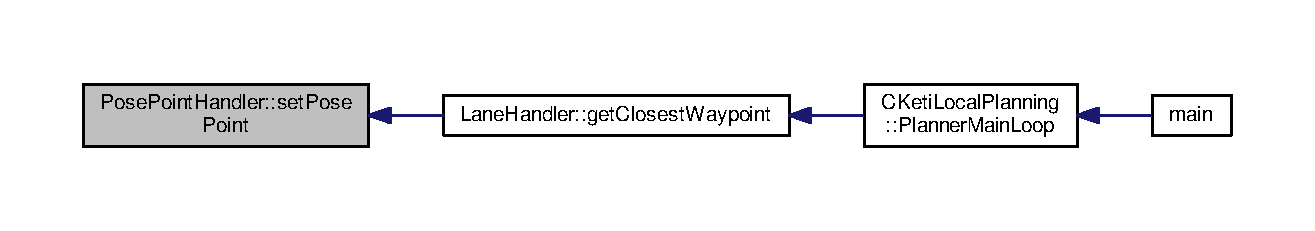
\includegraphics[width=350pt]{class_pose_point_handler_a6d037671a1c93d9d51a7b0e40eacd3fa_icgraph}
\end{center}
\end{figure}




\subsection{멤버 데이타 문서화}
\index{Pose\+Point\+Handler@{Pose\+Point\+Handler}!point\+\_\+@{point\+\_\+}}
\index{point\+\_\+@{point\+\_\+}!Pose\+Point\+Handler@{Pose\+Point\+Handler}}
\subsubsection[{\texorpdfstring{point\+\_\+}{point_}}]{\setlength{\rightskip}{0pt plus 5cm}geometry\+\_\+msgs\+::\+Point Pose\+Point\+Handler\+::point\+\_\+\hspace{0.3cm}{\ttfamily [private]}}\hypertarget{class_pose_point_handler_aa6dc915c1a9a98a64dd78c51f4b5ae02}{}\label{class_pose_point_handler_aa6dc915c1a9a98a64dd78c51f4b5ae02}


pose\+\_\+point\+\_\+handler.\+h 파일의 15 번째 라인에서 정의되었습니다.

\index{Pose\+Point\+Handler@{Pose\+Point\+Handler}!pose2\+\_\+@{pose2\+\_\+}}
\index{pose2\+\_\+@{pose2\+\_\+}!Pose\+Point\+Handler@{Pose\+Point\+Handler}}
\subsubsection[{\texorpdfstring{pose2\+\_\+}{pose2_}}]{\setlength{\rightskip}{0pt plus 5cm}geometry\+\_\+msgs\+::\+Pose Pose\+Point\+Handler\+::pose2\+\_\+\hspace{0.3cm}{\ttfamily [private]}}\hypertarget{class_pose_point_handler_ad615a2da1c3cd5cc3b5162390dac6136}{}\label{class_pose_point_handler_ad615a2da1c3cd5cc3b5162390dac6136}


pose\+\_\+point\+\_\+handler.\+h 파일의 14 번째 라인에서 정의되었습니다.

\index{Pose\+Point\+Handler@{Pose\+Point\+Handler}!pose\+\_\+@{pose\+\_\+}}
\index{pose\+\_\+@{pose\+\_\+}!Pose\+Point\+Handler@{Pose\+Point\+Handler}}
\subsubsection[{\texorpdfstring{pose\+\_\+}{pose_}}]{\setlength{\rightskip}{0pt plus 5cm}geometry\+\_\+msgs\+::\+Pose Pose\+Point\+Handler\+::pose\+\_\+\hspace{0.3cm}{\ttfamily [private]}}\hypertarget{class_pose_point_handler_ab78a62b6b03dee10487bf53339685a7d}{}\label{class_pose_point_handler_ab78a62b6b03dee10487bf53339685a7d}


pose\+\_\+point\+\_\+handler.\+h 파일의 13 번째 라인에서 정의되었습니다.



이 클래스에 대한 문서화 페이지는 다음의 파일들로부터 생성되었습니다.\+:\begin{DoxyCompactItemize}
\item 
/home/dallddungi/keti\+\_\+ws/src/keti\+\_\+local\+\_\+planning/include/data\+\_\+handler/\hyperlink{pose__point__handler_8h}{pose\+\_\+point\+\_\+handler.\+h}\item 
/home/dallddungi/keti\+\_\+ws/src/keti\+\_\+local\+\_\+planning/src/data\+\_\+handler/\hyperlink{pose__point__handler_8cpp}{pose\+\_\+point\+\_\+handler.\+cpp}\end{DoxyCompactItemize}

\hypertarget{class_ros_helpers}{}\section{Ros\+Helpers 클래스 참조}
\label{class_ros_helpers}\index{Ros\+Helpers@{Ros\+Helpers}}


{\ttfamily \#include $<$ros\+\_\+helpers.\+h$>$}



Ros\+Helpers에 대한 협력 다이어그램\+:\nopagebreak
\begin{figure}[H]
\begin{center}
\leavevmode
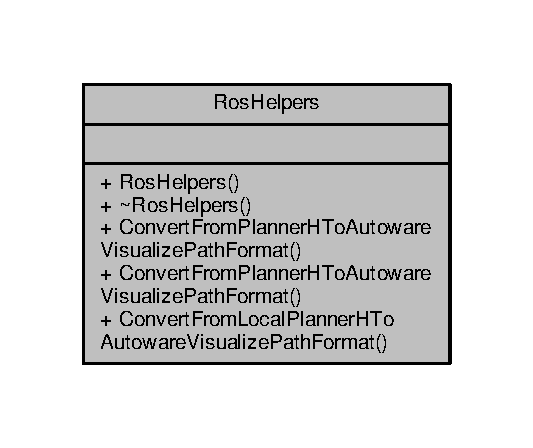
\includegraphics[width=256pt]{class_ros_helpers__coll__graph}
\end{center}
\end{figure}
\subsection*{Public 멤버 함수}
\begin{DoxyCompactItemize}
\item 
\hyperlink{class_ros_helpers_aee54c7b32e2c62ccc73e00f96a392f6f}{Ros\+Helpers} ()
\item 
virtual \hyperlink{class_ros_helpers_a8ffdfbb8effbdbbc162e5e3168faba84}{$\sim$\+Ros\+Helpers} ()
\end{DoxyCompactItemize}
\subsection*{정적 Public 멤버 함수}
\begin{DoxyCompactItemize}
\item 
static void \hyperlink{class_ros_helpers_ad82466a16ba11fded30d109a52b75074}{Convert\+From\+Planner\+H\+To\+Autoware\+Visualize\+Path\+Format} (const std\+::vector$<$ std\+::vector$<$ \hyperlink{class_way_point}{Way\+Point} $>$ $>$ \&global\+Paths, visualization\+\_\+msgs\+::\+Marker\+Array \&marker\+Array)
\item 
static void \hyperlink{class_ros_helpers_a88faef5f185405585e3394c9bf2feb36}{Convert\+From\+Planner\+H\+To\+Autoware\+Visualize\+Path\+Format} (const std\+::vector$<$ \hyperlink{class_way_point}{Way\+Point} $>$ \&global\+Paths, visualization\+\_\+msgs\+::\+Marker\+Array \&marker\+Array)
\item 
static void \hyperlink{class_ros_helpers_a00357e856ae16110fd9f3787cc3802d3}{Convert\+From\+Local\+Planner\+H\+To\+Autoware\+Visualize\+Path\+Format} (const std\+::vector$<$ \hyperlink{class_way_point}{Way\+Point} $>$ \&paths, visualization\+\_\+msgs\+::\+Marker\+Array \&marker\+Array)
\end{DoxyCompactItemize}


\subsection{상세한 설명}


ros\+\_\+helpers.\+h 파일의 8 번째 라인에서 정의되었습니다.



\subsection{생성자 \& 소멸자 문서화}
\index{Ros\+Helpers@{Ros\+Helpers}!Ros\+Helpers@{Ros\+Helpers}}
\index{Ros\+Helpers@{Ros\+Helpers}!Ros\+Helpers@{Ros\+Helpers}}
\subsubsection[{\texorpdfstring{Ros\+Helpers()}{RosHelpers()}}]{\setlength{\rightskip}{0pt plus 5cm}Ros\+Helpers\+::\+Ros\+Helpers (
\begin{DoxyParamCaption}
{}
\end{DoxyParamCaption}
)}\hypertarget{class_ros_helpers_aee54c7b32e2c62ccc73e00f96a392f6f}{}\label{class_ros_helpers_aee54c7b32e2c62ccc73e00f96a392f6f}


ros\+\_\+helpers.\+cpp 파일의 3 번째 라인에서 정의되었습니다.


\begin{DoxyCode}
3                        \{
4 
5 \}
\end{DoxyCode}
\index{Ros\+Helpers@{Ros\+Helpers}!````~Ros\+Helpers@{$\sim$\+Ros\+Helpers}}
\index{````~Ros\+Helpers@{$\sim$\+Ros\+Helpers}!Ros\+Helpers@{Ros\+Helpers}}
\subsubsection[{\texorpdfstring{$\sim$\+Ros\+Helpers()}{~RosHelpers()}}]{\setlength{\rightskip}{0pt plus 5cm}Ros\+Helpers\+::$\sim$\+Ros\+Helpers (
\begin{DoxyParamCaption}
{}
\end{DoxyParamCaption}
)\hspace{0.3cm}{\ttfamily [virtual]}}\hypertarget{class_ros_helpers_a8ffdfbb8effbdbbc162e5e3168faba84}{}\label{class_ros_helpers_a8ffdfbb8effbdbbc162e5e3168faba84}


ros\+\_\+helpers.\+cpp 파일의 7 번째 라인에서 정의되었습니다.


\begin{DoxyCode}
7                         \{
8 \}
\end{DoxyCode}


\subsection{멤버 함수 문서화}
\index{Ros\+Helpers@{Ros\+Helpers}!Convert\+From\+Local\+Planner\+H\+To\+Autoware\+Visualize\+Path\+Format@{Convert\+From\+Local\+Planner\+H\+To\+Autoware\+Visualize\+Path\+Format}}
\index{Convert\+From\+Local\+Planner\+H\+To\+Autoware\+Visualize\+Path\+Format@{Convert\+From\+Local\+Planner\+H\+To\+Autoware\+Visualize\+Path\+Format}!Ros\+Helpers@{Ros\+Helpers}}
\subsubsection[{\texorpdfstring{Convert\+From\+Local\+Planner\+H\+To\+Autoware\+Visualize\+Path\+Format(const std\+::vector$<$ Way\+Point $>$ \&paths, visualization\+\_\+msgs\+::\+Marker\+Array \&marker\+Array)}{ConvertFromLocalPlannerHToAutowareVisualizePathFormat(const std::vector< WayPoint > &paths, visualization_msgs::MarkerArray &markerArray)}}]{\setlength{\rightskip}{0pt plus 5cm}void Ros\+Helpers\+::\+Convert\+From\+Local\+Planner\+H\+To\+Autoware\+Visualize\+Path\+Format (
\begin{DoxyParamCaption}
\item[{const std\+::vector$<$ {\bf Way\+Point} $>$ \&}]{paths, }
\item[{visualization\+\_\+msgs\+::\+Marker\+Array \&}]{marker\+Array}
\end{DoxyParamCaption}
)\hspace{0.3cm}{\ttfamily [static]}}\hypertarget{class_ros_helpers_a00357e856ae16110fd9f3787cc3802d3}{}\label{class_ros_helpers_a00357e856ae16110fd9f3787cc3802d3}


ros\+\_\+helpers.\+cpp 파일의 94 번째 라인에서 정의되었습니다.


\begin{DoxyCode}
97 \{
98   visualization\_msgs::Marker lane\_waypoint\_marker;
99   lane\_waypoint\_marker.header.frame\_id = \textcolor{stringliteral}{"map"};
100   lane\_waypoint\_marker.header.stamp = ros::Time();
101   lane\_waypoint\_marker.ns = \textcolor{stringliteral}{"global\_lane\_array\_marker"};
102   lane\_waypoint\_marker.type = visualization\_msgs::Marker::LINE\_STRIP;
103   lane\_waypoint\_marker.action = visualization\_msgs::Marker::ADD;
104   lane\_waypoint\_marker.scale.x = 0.1;
105   lane\_waypoint\_marker.scale.y = 0.1;
106   \textcolor{comment}{//lane\_waypoint\_marker.scale.z = 0.1;}
107   lane\_waypoint\_marker.frame\_locked = \textcolor{keyword}{false};
108   std\_msgs::ColorRGBA  total\_color, curr\_color;
109 
110 
111   lane\_waypoint\_marker.points.clear();
112   lane\_waypoint\_marker.id = 1;
113 
114   \textcolor{keywordflow}{for} (\textcolor{keywordtype}{unsigned} \textcolor{keywordtype}{int} j=0; j < paths.size(); j++)
115   \{
116     geometry\_msgs::Point point;
117 
118     point.x = paths.at(j).pos\_.x\_;
119     point.y = paths.at(j).pos\_.y\_;
120     point.z = paths.at(j).pos\_.z\_;
121 
122     lane\_waypoint\_marker.points.push\_back(point);
123   \}
124 
125   lane\_waypoint\_marker.color.a = 0.9;
126   lane\_waypoint\_marker.color.r = 0.0;
127   lane\_waypoint\_marker.color.g = 1.0;
128   lane\_waypoint\_marker.color.b = 0;
129 
130   markerArray.markers.push\_back(lane\_waypoint\_marker);
131 
132 \}
\end{DoxyCode}


이 함수를 호출하는 함수들에 대한 그래프입니다.\+:\nopagebreak
\begin{figure}[H]
\begin{center}
\leavevmode
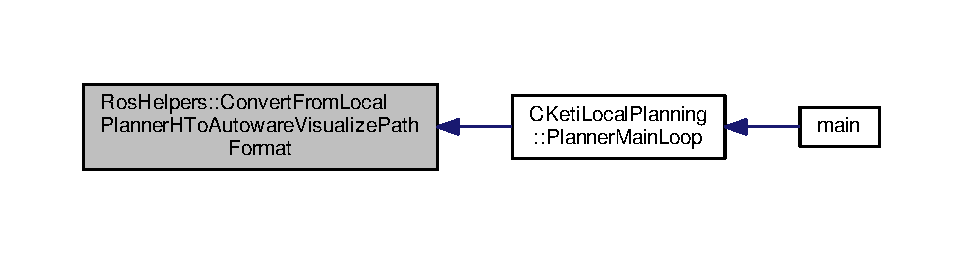
\includegraphics[width=350pt]{class_ros_helpers_a00357e856ae16110fd9f3787cc3802d3_icgraph}
\end{center}
\end{figure}


\index{Ros\+Helpers@{Ros\+Helpers}!Convert\+From\+Planner\+H\+To\+Autoware\+Visualize\+Path\+Format@{Convert\+From\+Planner\+H\+To\+Autoware\+Visualize\+Path\+Format}}
\index{Convert\+From\+Planner\+H\+To\+Autoware\+Visualize\+Path\+Format@{Convert\+From\+Planner\+H\+To\+Autoware\+Visualize\+Path\+Format}!Ros\+Helpers@{Ros\+Helpers}}
\subsubsection[{\texorpdfstring{Convert\+From\+Planner\+H\+To\+Autoware\+Visualize\+Path\+Format(const std\+::vector$<$ std\+::vector$<$ Way\+Point $>$ $>$ \&global\+Paths, visualization\+\_\+msgs\+::\+Marker\+Array \&marker\+Array)}{ConvertFromPlannerHToAutowareVisualizePathFormat(const std::vector< std::vector< WayPoint > > &globalPaths, visualization_msgs::MarkerArray &markerArray)}}]{\setlength{\rightskip}{0pt plus 5cm}void Ros\+Helpers\+::\+Convert\+From\+Planner\+H\+To\+Autoware\+Visualize\+Path\+Format (
\begin{DoxyParamCaption}
\item[{const std\+::vector$<$ std\+::vector$<$ {\bf Way\+Point} $>$ $>$ \&}]{global\+Paths, }
\item[{visualization\+\_\+msgs\+::\+Marker\+Array \&}]{marker\+Array}
\end{DoxyParamCaption}
)\hspace{0.3cm}{\ttfamily [static]}}\hypertarget{class_ros_helpers_ad82466a16ba11fded30d109a52b75074}{}\label{class_ros_helpers_ad82466a16ba11fded30d109a52b75074}


ros\+\_\+helpers.\+cpp 파일의 11 번째 라인에서 정의되었습니다.


\begin{DoxyCode}
13 \{
14   visualization\_msgs::Marker lane\_waypoint\_marker;
15   lane\_waypoint\_marker.header.frame\_id = \textcolor{stringliteral}{"map"};
16   lane\_waypoint\_marker.header.stamp = ros::Time();
17   lane\_waypoint\_marker.ns = \textcolor{stringliteral}{"global\_lane\_array\_marker"};
18   lane\_waypoint\_marker.type = visualization\_msgs::Marker::LINE\_STRIP;
19   lane\_waypoint\_marker.action = visualization\_msgs::Marker::ADD;
20 
21 
22   std\_msgs::ColorRGBA roll\_color, total\_color, curr\_color;
23   lane\_waypoint\_marker.points.clear();
24   lane\_waypoint\_marker.id = 1;
25   lane\_waypoint\_marker.scale.x = 0.1;
26   lane\_waypoint\_marker.scale.y = 0.1;
27   total\_color.r = 1;
28   total\_color.g = 0;
29   total\_color.b = 0;
30   total\_color.a = 0.5;
31   lane\_waypoint\_marker.color = total\_color;
32   lane\_waypoint\_marker.frame\_locked = \textcolor{keyword}{false};
33 
34   \textcolor{keywordtype}{int} count = 0;
35   \textcolor{keywordflow}{for} (\textcolor{keywordtype}{unsigned} \textcolor{keywordtype}{int} i = 0; i < globalPaths.size(); i++)
36   \{
37     lane\_waypoint\_marker.points.clear();
38     lane\_waypoint\_marker.id = count;
39 
40     \textcolor{keywordflow}{for} (\textcolor{keywordtype}{unsigned} \textcolor{keywordtype}{int} j=0; j < globalPaths.at(i).size(); j++)
41     \{
42       geometry\_msgs::Point point;
43 
44       point.x = globalPaths.at(i).at(j).pos\_.x\_;
45       point.y = globalPaths.at(i).at(j).pos\_.y\_;
46       point.z = globalPaths.at(i).at(j).pos\_.z\_;
47 
48       lane\_waypoint\_marker.points.push\_back(point);
49     \}
50 
51     markerArray.markers.push\_back(lane\_waypoint\_marker);
52     count++;
53   \}
54 \}
\end{DoxyCode}


이 함수를 호출하는 함수들에 대한 그래프입니다.\+:\nopagebreak
\begin{figure}[H]
\begin{center}
\leavevmode
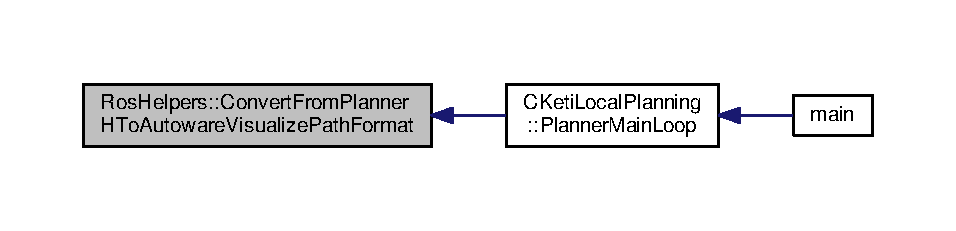
\includegraphics[width=350pt]{class_ros_helpers_ad82466a16ba11fded30d109a52b75074_icgraph}
\end{center}
\end{figure}


\index{Ros\+Helpers@{Ros\+Helpers}!Convert\+From\+Planner\+H\+To\+Autoware\+Visualize\+Path\+Format@{Convert\+From\+Planner\+H\+To\+Autoware\+Visualize\+Path\+Format}}
\index{Convert\+From\+Planner\+H\+To\+Autoware\+Visualize\+Path\+Format@{Convert\+From\+Planner\+H\+To\+Autoware\+Visualize\+Path\+Format}!Ros\+Helpers@{Ros\+Helpers}}
\subsubsection[{\texorpdfstring{Convert\+From\+Planner\+H\+To\+Autoware\+Visualize\+Path\+Format(const std\+::vector$<$ Way\+Point $>$ \&global\+Paths, visualization\+\_\+msgs\+::\+Marker\+Array \&marker\+Array)}{ConvertFromPlannerHToAutowareVisualizePathFormat(const std::vector< WayPoint > &globalPaths, visualization_msgs::MarkerArray &markerArray)}}]{\setlength{\rightskip}{0pt plus 5cm}void Ros\+Helpers\+::\+Convert\+From\+Planner\+H\+To\+Autoware\+Visualize\+Path\+Format (
\begin{DoxyParamCaption}
\item[{const std\+::vector$<$ {\bf Way\+Point} $>$ \&}]{global\+Paths, }
\item[{visualization\+\_\+msgs\+::\+Marker\+Array \&}]{marker\+Array}
\end{DoxyParamCaption}
)\hspace{0.3cm}{\ttfamily [static]}}\hypertarget{class_ros_helpers_a88faef5f185405585e3394c9bf2feb36}{}\label{class_ros_helpers_a88faef5f185405585e3394c9bf2feb36}


ros\+\_\+helpers.\+cpp 파일의 57 번째 라인에서 정의되었습니다.


\begin{DoxyCode}
59 \{
60   visualization\_msgs::Marker lane\_waypoint\_marker;
61   lane\_waypoint\_marker.header.frame\_id = \textcolor{stringliteral}{"map"};
62   lane\_waypoint\_marker.header.stamp = ros::Time();
63   lane\_waypoint\_marker.ns = \textcolor{stringliteral}{"global\_lane\_array\_marker"};
64   lane\_waypoint\_marker.type = visualization\_msgs::Marker::LINE\_STRIP;
65   lane\_waypoint\_marker.action = visualization\_msgs::Marker::ADD;
66 
67 
68   std\_msgs::ColorRGBA roll\_color, total\_color, curr\_color;
69   lane\_waypoint\_marker.points.clear();
70   lane\_waypoint\_marker.id = 1;
71   lane\_waypoint\_marker.scale.x = 0.1;
72   lane\_waypoint\_marker.scale.y = 0.1;
73   total\_color.r = 1;
74   total\_color.g = 0;
75   total\_color.b = 0;
76   total\_color.a = 0.5;
77   lane\_waypoint\_marker.color = total\_color;
78   lane\_waypoint\_marker.frame\_locked = \textcolor{keyword}{false};
79 
80   \textcolor{keywordflow}{for} (\textcolor{keywordtype}{unsigned} \textcolor{keywordtype}{int} j=0; j < globalPaths.size(); j++)
81   \{
82     geometry\_msgs::Point point;
83 
84     point.x = globalPaths.at(j).pos\_.x\_;
85     point.y = globalPaths.at(j).pos\_.y\_;
86     point.z = globalPaths.at(j).pos\_.z\_;
87 
88     lane\_waypoint\_marker.points.push\_back(point);
89   \}
90   markerArray.markers.push\_back(lane\_waypoint\_marker);
91 \}
\end{DoxyCode}


이 클래스에 대한 문서화 페이지는 다음의 파일들로부터 생성되었습니다.\+:\begin{DoxyCompactItemize}
\item 
/home/dallddungi/keti\+\_\+ws/src/keti\+\_\+local\+\_\+planning/include/\hyperlink{ros__helpers_8h}{ros\+\_\+helpers.\+h}\item 
/home/dallddungi/keti\+\_\+ws/src/keti\+\_\+local\+\_\+planning/src/\hyperlink{ros__helpers_8cpp}{ros\+\_\+helpers.\+cpp}\end{DoxyCompactItemize}

\hypertarget{class_way_point}{}\section{Way\+Point 클래스 참조}
\label{class_way_point}\index{Way\+Point@{Way\+Point}}


type representing class containing (\hyperlink{class_g_p_s_point}{G\+P\+S\+Point}, v)  




{\ttfamily \#include $<$waypoint.\+h$>$}



Way\+Point에 대한 협력 다이어그램\+:\nopagebreak
\begin{figure}[H]
\begin{center}
\leavevmode
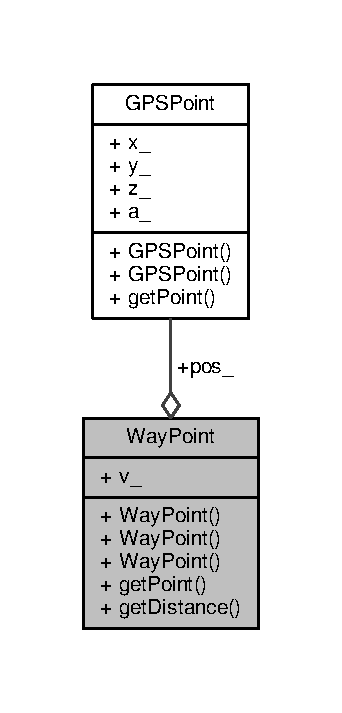
\includegraphics[width=164pt]{class_way_point__coll__graph}
\end{center}
\end{figure}
\subsection*{Public 멤버 함수}
\begin{DoxyCompactItemize}
\item 
\hyperlink{class_way_point_a0388a615719454d38b5a8160d8058550}{Way\+Point} ()
\item 
\hyperlink{class_way_point_a0a5358f5f8894bf9bc0279e4758f712d}{Way\+Point} (const double \&x, const double \&y, const double \&z, const double \&a)
\item 
\hyperlink{class_way_point_afb55bf3008e6df983912ca195a4994e1}{Way\+Point} (const double \&x, const double \&y, const double \&z, const double \&a, const double \&v)
\item 
geometry\+\_\+msgs\+::\+Point \hyperlink{class_way_point_a3d0e6433de5c74a13be5f6f276d0a71d}{get\+Point} ()
\item 
double \hyperlink{class_way_point_ad2b8fa2161cb6dfa5d7ff8f993f1c62c}{get\+Distance} (geometry\+\_\+msgs\+::\+Point point)
\end{DoxyCompactItemize}
\subsection*{Public 속성}
\begin{DoxyCompactItemize}
\item 
\hyperlink{class_g_p_s_point}{G\+P\+S\+Point} \hyperlink{class_way_point_aef2ddd64bef263157f27d69e40f1e7e3}{pos\+\_\+}
\item 
double \hyperlink{class_way_point_aecad0ca0d0dbb03cf02d92d31e5e99bd}{v\+\_\+}
\end{DoxyCompactItemize}


\subsection{상세한 설명}
type representing class containing (\hyperlink{class_g_p_s_point}{G\+P\+S\+Point}, v) 

waypoint.\+h 파일의 10 번째 라인에서 정의되었습니다.



\subsection{생성자 \& 소멸자 문서화}
\index{Way\+Point@{Way\+Point}!Way\+Point@{Way\+Point}}
\index{Way\+Point@{Way\+Point}!Way\+Point@{Way\+Point}}
\subsubsection[{\texorpdfstring{Way\+Point()}{WayPoint()}}]{\setlength{\rightskip}{0pt plus 5cm}Way\+Point\+::\+Way\+Point (
\begin{DoxyParamCaption}
{}
\end{DoxyParamCaption}
)\hspace{0.3cm}{\ttfamily [inline]}}\hypertarget{class_way_point_a0388a615719454d38b5a8160d8058550}{}\label{class_way_point_a0388a615719454d38b5a8160d8058550}


waypoint.\+h 파일의 15 번째 라인에서 정의되었습니다.


\begin{DoxyCode}
16   \{
17 
18   \}
\end{DoxyCode}
\index{Way\+Point@{Way\+Point}!Way\+Point@{Way\+Point}}
\index{Way\+Point@{Way\+Point}!Way\+Point@{Way\+Point}}
\subsubsection[{\texorpdfstring{Way\+Point(const double \&x, const double \&y, const double \&z, const double \&a)}{WayPoint(const double &x, const double &y, const double &z, const double &a)}}]{\setlength{\rightskip}{0pt plus 5cm}Way\+Point\+::\+Way\+Point (
\begin{DoxyParamCaption}
\item[{const double \&}]{x, }
\item[{const double \&}]{y, }
\item[{const double \&}]{z, }
\item[{const double \&}]{a}
\end{DoxyParamCaption}
)\hspace{0.3cm}{\ttfamily [inline]}}\hypertarget{class_way_point_a0a5358f5f8894bf9bc0279e4758f712d}{}\label{class_way_point_a0a5358f5f8894bf9bc0279e4758f712d}


waypoint.\+h 파일의 19 번째 라인에서 정의되었습니다.


\begin{DoxyCode}
20   \{
21     \hyperlink{class_way_point_aef2ddd64bef263157f27d69e40f1e7e3}{pos\_}.\hyperlink{class_g_p_s_point_ad4b7325afe1ca0fcf8d2ef284ab9b62c}{x\_} = x;
22     \hyperlink{class_way_point_aef2ddd64bef263157f27d69e40f1e7e3}{pos\_}.\hyperlink{class_g_p_s_point_ad41d0e7a93f8766181402ce25af798fe}{y\_} = y;
23     \hyperlink{class_way_point_aef2ddd64bef263157f27d69e40f1e7e3}{pos\_}.\hyperlink{class_g_p_s_point_aa6622ef5c0c58fa1b59c1d5b77fe020c}{z\_} = z;
24     \hyperlink{class_way_point_aef2ddd64bef263157f27d69e40f1e7e3}{pos\_}.\hyperlink{class_g_p_s_point_ac4652d53d65aeb605f7eb35128a5ab90}{a\_} = a;
25   \}
\end{DoxyCode}
\index{Way\+Point@{Way\+Point}!Way\+Point@{Way\+Point}}
\index{Way\+Point@{Way\+Point}!Way\+Point@{Way\+Point}}
\subsubsection[{\texorpdfstring{Way\+Point(const double \&x, const double \&y, const double \&z, const double \&a, const double \&v)}{WayPoint(const double &x, const double &y, const double &z, const double &a, const double &v)}}]{\setlength{\rightskip}{0pt plus 5cm}Way\+Point\+::\+Way\+Point (
\begin{DoxyParamCaption}
\item[{const double \&}]{x, }
\item[{const double \&}]{y, }
\item[{const double \&}]{z, }
\item[{const double \&}]{a, }
\item[{const double \&}]{v}
\end{DoxyParamCaption}
)\hspace{0.3cm}{\ttfamily [inline]}}\hypertarget{class_way_point_afb55bf3008e6df983912ca195a4994e1}{}\label{class_way_point_afb55bf3008e6df983912ca195a4994e1}


waypoint.\+h 파일의 26 번째 라인에서 정의되었습니다.


\begin{DoxyCode}
27   \{
28     \hyperlink{class_way_point_aef2ddd64bef263157f27d69e40f1e7e3}{pos\_}.\hyperlink{class_g_p_s_point_ad4b7325afe1ca0fcf8d2ef284ab9b62c}{x\_} = x;
29     \hyperlink{class_way_point_aef2ddd64bef263157f27d69e40f1e7e3}{pos\_}.\hyperlink{class_g_p_s_point_ad41d0e7a93f8766181402ce25af798fe}{y\_} = y;
30     \hyperlink{class_way_point_aef2ddd64bef263157f27d69e40f1e7e3}{pos\_}.\hyperlink{class_g_p_s_point_aa6622ef5c0c58fa1b59c1d5b77fe020c}{z\_} = z;
31     \hyperlink{class_way_point_aef2ddd64bef263157f27d69e40f1e7e3}{pos\_}.\hyperlink{class_g_p_s_point_ac4652d53d65aeb605f7eb35128a5ab90}{a\_} = a;
32     \hyperlink{class_way_point_aecad0ca0d0dbb03cf02d92d31e5e99bd}{v\_} = v;
33   \}
\end{DoxyCode}


\subsection{멤버 함수 문서화}
\index{Way\+Point@{Way\+Point}!get\+Distance@{get\+Distance}}
\index{get\+Distance@{get\+Distance}!Way\+Point@{Way\+Point}}
\subsubsection[{\texorpdfstring{get\+Distance(geometry\+\_\+msgs\+::\+Point point)}{getDistance(geometry_msgs::Point point)}}]{\setlength{\rightskip}{0pt plus 5cm}double Way\+Point\+::get\+Distance (
\begin{DoxyParamCaption}
\item[{geometry\+\_\+msgs\+::\+Point}]{point}
\end{DoxyParamCaption}
)\hspace{0.3cm}{\ttfamily [inline]}}\hypertarget{class_way_point_ad2b8fa2161cb6dfa5d7ff8f993f1c62c}{}\label{class_way_point_ad2b8fa2161cb6dfa5d7ff8f993f1c62c}


waypoint.\+h 파일의 43 번째 라인에서 정의되었습니다.


\begin{DoxyCode}
44   \{
45     \textcolor{keywordflow}{return} sqrt(pow(point.x-\hyperlink{class_way_point_aef2ddd64bef263157f27d69e40f1e7e3}{pos\_}.\hyperlink{class_g_p_s_point_ad4b7325afe1ca0fcf8d2ef284ab9b62c}{x\_},2)+pow(point.y-\hyperlink{class_way_point_aef2ddd64bef263157f27d69e40f1e7e3}{pos\_}.\hyperlink{class_g_p_s_point_ad41d0e7a93f8766181402ce25af798fe}{y\_},2)+pow(point.z-
      \hyperlink{class_way_point_aef2ddd64bef263157f27d69e40f1e7e3}{pos\_}.\hyperlink{class_g_p_s_point_aa6622ef5c0c58fa1b59c1d5b77fe020c}{z\_},2));
46   \}
\end{DoxyCode}
\index{Way\+Point@{Way\+Point}!get\+Point@{get\+Point}}
\index{get\+Point@{get\+Point}!Way\+Point@{Way\+Point}}
\subsubsection[{\texorpdfstring{get\+Point()}{getPoint()}}]{\setlength{\rightskip}{0pt plus 5cm}geometry\+\_\+msgs\+::\+Point Way\+Point\+::get\+Point (
\begin{DoxyParamCaption}
{}
\end{DoxyParamCaption}
)\hspace{0.3cm}{\ttfamily [inline]}}\hypertarget{class_way_point_a3d0e6433de5c74a13be5f6f276d0a71d}{}\label{class_way_point_a3d0e6433de5c74a13be5f6f276d0a71d}


waypoint.\+h 파일의 34 번째 라인에서 정의되었습니다.


\begin{DoxyCode}
35   \{
36     geometry\_msgs::Point pt;
37     pt.x = \hyperlink{class_way_point_aef2ddd64bef263157f27d69e40f1e7e3}{pos\_}.\hyperlink{class_g_p_s_point_ad4b7325afe1ca0fcf8d2ef284ab9b62c}{x\_};
38     pt.y = \hyperlink{class_way_point_aef2ddd64bef263157f27d69e40f1e7e3}{pos\_}.\hyperlink{class_g_p_s_point_ad41d0e7a93f8766181402ce25af798fe}{y\_};
39     pt.z = \hyperlink{class_way_point_aef2ddd64bef263157f27d69e40f1e7e3}{pos\_}.\hyperlink{class_g_p_s_point_aa6622ef5c0c58fa1b59c1d5b77fe020c}{z\_};
40     \textcolor{keywordflow}{return} pt;
41   \}
\end{DoxyCode}


\subsection{멤버 데이타 문서화}
\index{Way\+Point@{Way\+Point}!pos\+\_\+@{pos\+\_\+}}
\index{pos\+\_\+@{pos\+\_\+}!Way\+Point@{Way\+Point}}
\subsubsection[{\texorpdfstring{pos\+\_\+}{pos_}}]{\setlength{\rightskip}{0pt plus 5cm}{\bf G\+P\+S\+Point} Way\+Point\+::pos\+\_\+}\hypertarget{class_way_point_aef2ddd64bef263157f27d69e40f1e7e3}{}\label{class_way_point_aef2ddd64bef263157f27d69e40f1e7e3}


waypoint.\+h 파일의 13 번째 라인에서 정의되었습니다.

\index{Way\+Point@{Way\+Point}!v\+\_\+@{v\+\_\+}}
\index{v\+\_\+@{v\+\_\+}!Way\+Point@{Way\+Point}}
\subsubsection[{\texorpdfstring{v\+\_\+}{v_}}]{\setlength{\rightskip}{0pt plus 5cm}double Way\+Point\+::v\+\_\+}\hypertarget{class_way_point_aecad0ca0d0dbb03cf02d92d31e5e99bd}{}\label{class_way_point_aecad0ca0d0dbb03cf02d92d31e5e99bd}


waypoint.\+h 파일의 14 번째 라인에서 정의되었습니다.



이 클래스에 대한 문서화 페이지는 다음의 파일로부터 생성되었습니다.\+:\begin{DoxyCompactItemize}
\item 
/home/dallddungi/keti\+\_\+ws/src/keti\+\_\+local\+\_\+planning/include/data\+\_\+classes/\hyperlink{waypoint_8h}{waypoint.\+h}\end{DoxyCompactItemize}

\chapter{파일 문서화}
\hypertarget{cketilocalplanning_8h}{}\section{/home/dallddungi/keti\+\_\+ws/src/keti\+\_\+local\+\_\+planning/include/cketilocalplanning.h 파일 참조}
\label{cketilocalplanning_8h}\index{/home/dallddungi/keti\+\_\+ws/src/keti\+\_\+local\+\_\+planning/include/cketilocalplanning.\+h@{/home/dallddungi/keti\+\_\+ws/src/keti\+\_\+local\+\_\+planning/include/cketilocalplanning.\+h}}
{\ttfamily \#include $<$ros/ros.\+h$>$}\\*
{\ttfamily \#include $<$geometry\+\_\+msgs/\+Pose\+Stamped.\+h$>$}\\*
{\ttfamily \#include \char`\"{}autoware\+\_\+msgs/\+Lane\+Array.\+h\char`\"{}}\\*
{\ttfamily \#include \char`\"{}data\+\_\+handler/lanearray\+\_\+handler.\+h\char`\"{}}\\*
{\ttfamily \#include \char`\"{}data\+\_\+handler/lane\+\_\+handler.\+h\char`\"{}}\\*
cketilocalplanning.\+h에 대한 include 의존 그래프\nopagebreak
\begin{figure}[H]
\begin{center}
\leavevmode
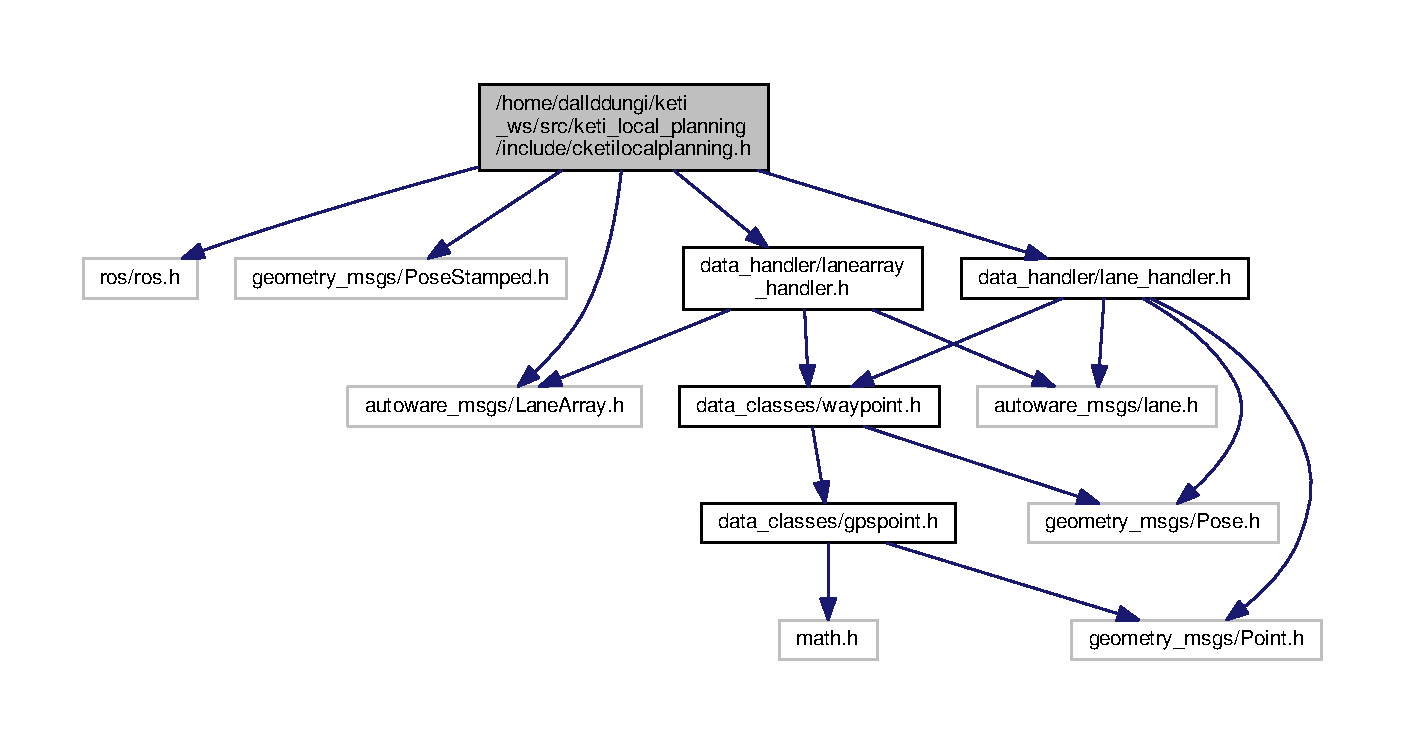
\includegraphics[width=350pt]{cketilocalplanning_8h__incl}
\end{center}
\end{figure}
이 그래프는 이 파일을 직/간접적으로 include 하는 파일들을 보여줍니다.\+:\nopagebreak
\begin{figure}[H]
\begin{center}
\leavevmode
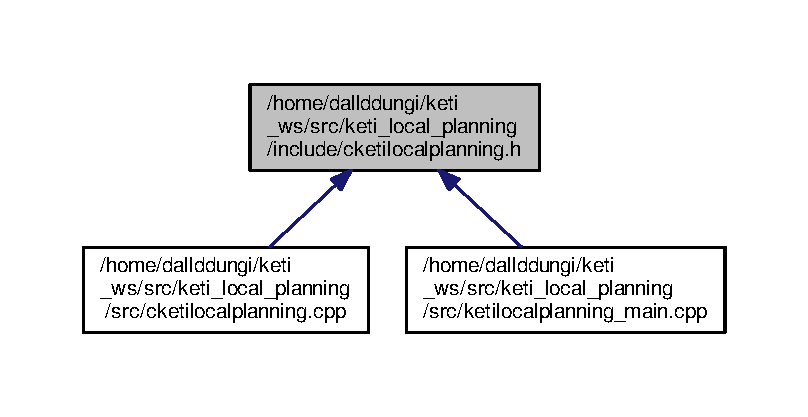
\includegraphics[width=350pt]{cketilocalplanning_8h__dep__incl}
\end{center}
\end{figure}
\subsection*{클래스}
\begin{DoxyCompactItemize}
\item 
class \hyperlink{class_c_keti_local_planning}{C\+Keti\+Local\+Planning}
\begin{DoxyCompactList}\small\item\em Planning local path avoiding obstacle and following lane. \end{DoxyCompactList}\end{DoxyCompactItemize}

\hypertarget{gpspoint_8h}{}\section{/home/dallddungi/keti\+\_\+ws/src/keti\+\_\+local\+\_\+planning/include/data\+\_\+classes/gpspoint.h 파일 참조}
\label{gpspoint_8h}\index{/home/dallddungi/keti\+\_\+ws/src/keti\+\_\+local\+\_\+planning/include/data\+\_\+classes/gpspoint.\+h@{/home/dallddungi/keti\+\_\+ws/src/keti\+\_\+local\+\_\+planning/include/data\+\_\+classes/gpspoint.\+h}}
{\ttfamily \#include $<$math.\+h$>$}\\*
{\ttfamily \#include $<$geometry\+\_\+msgs/\+Point.\+h$>$}\\*
gpspoint.\+h에 대한 include 의존 그래프\nopagebreak
\begin{figure}[H]
\begin{center}
\leavevmode
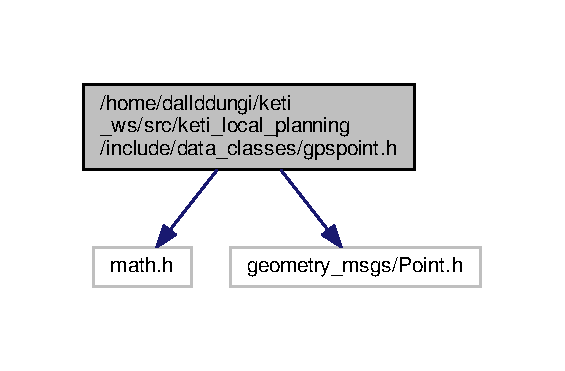
\includegraphics[width=271pt]{gpspoint_8h__incl}
\end{center}
\end{figure}
이 그래프는 이 파일을 직/간접적으로 include 하는 파일들을 보여줍니다.\+:\nopagebreak
\begin{figure}[H]
\begin{center}
\leavevmode
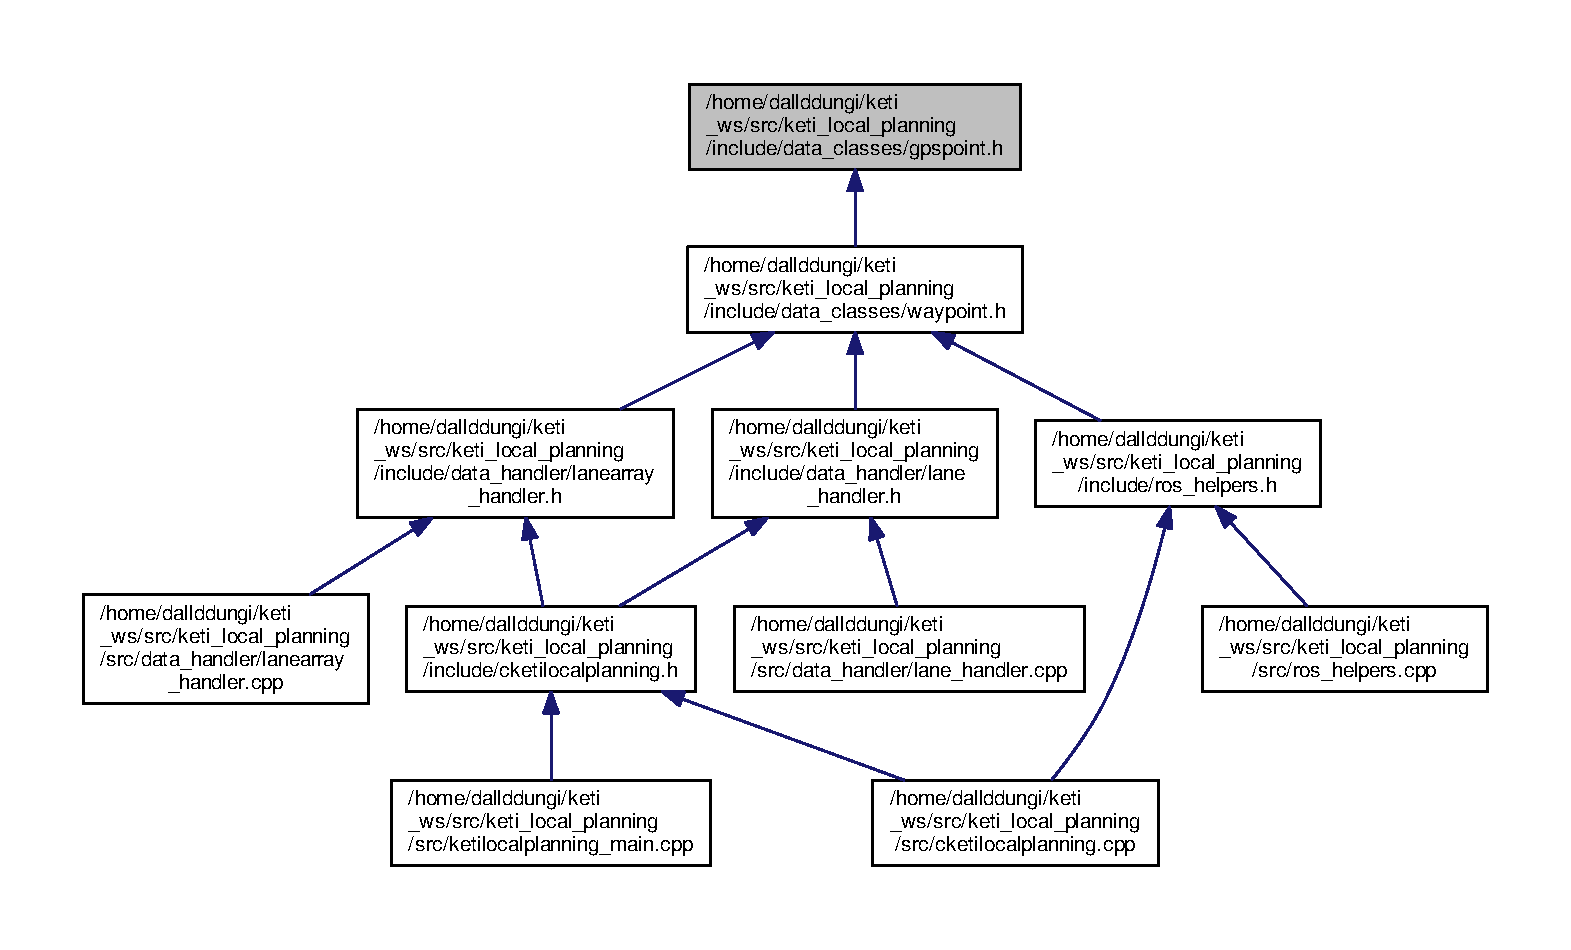
\includegraphics[width=350pt]{gpspoint_8h__dep__incl}
\end{center}
\end{figure}
\subsection*{클래스}
\begin{DoxyCompactItemize}
\item 
class \hyperlink{class_g_p_s_point}{G\+P\+S\+Point}
\begin{DoxyCompactList}\small\item\em type representing class containing (x,y,z,a) \end{DoxyCompactList}\end{DoxyCompactItemize}

\hypertarget{waypoint_8h}{}\section{/home/dallddungi/keti\+\_\+ws/src/keti\+\_\+local\+\_\+planning/include/data\+\_\+classes/waypoint.h 파일 참조}
\label{waypoint_8h}\index{/home/dallddungi/keti\+\_\+ws/src/keti\+\_\+local\+\_\+planning/include/data\+\_\+classes/waypoint.\+h@{/home/dallddungi/keti\+\_\+ws/src/keti\+\_\+local\+\_\+planning/include/data\+\_\+classes/waypoint.\+h}}
{\ttfamily \#include \char`\"{}data\+\_\+classes/gpspoint.\+h\char`\"{}}\\*
{\ttfamily \#include \char`\"{}geometry\+\_\+msgs/\+Pose.\+h\char`\"{}}\\*
waypoint.\+h에 대한 include 의존 그래프\nopagebreak
\begin{figure}[H]
\begin{center}
\leavevmode
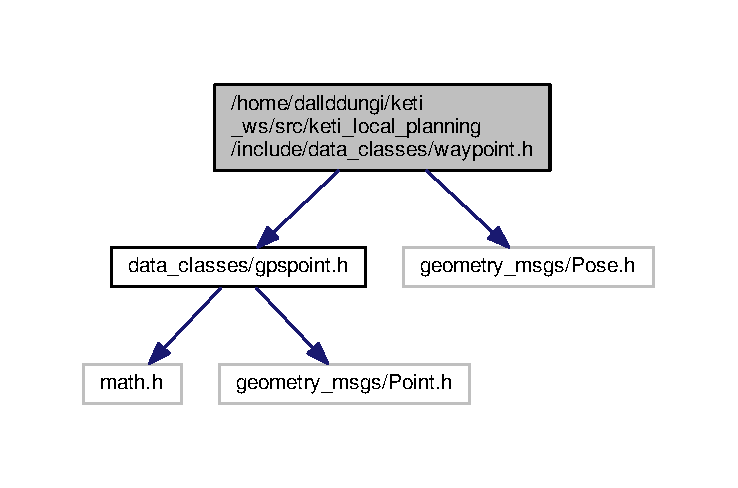
\includegraphics[width=350pt]{waypoint_8h__incl}
\end{center}
\end{figure}
이 그래프는 이 파일을 직/간접적으로 include 하는 파일들을 보여줍니다.\+:\nopagebreak
\begin{figure}[H]
\begin{center}
\leavevmode
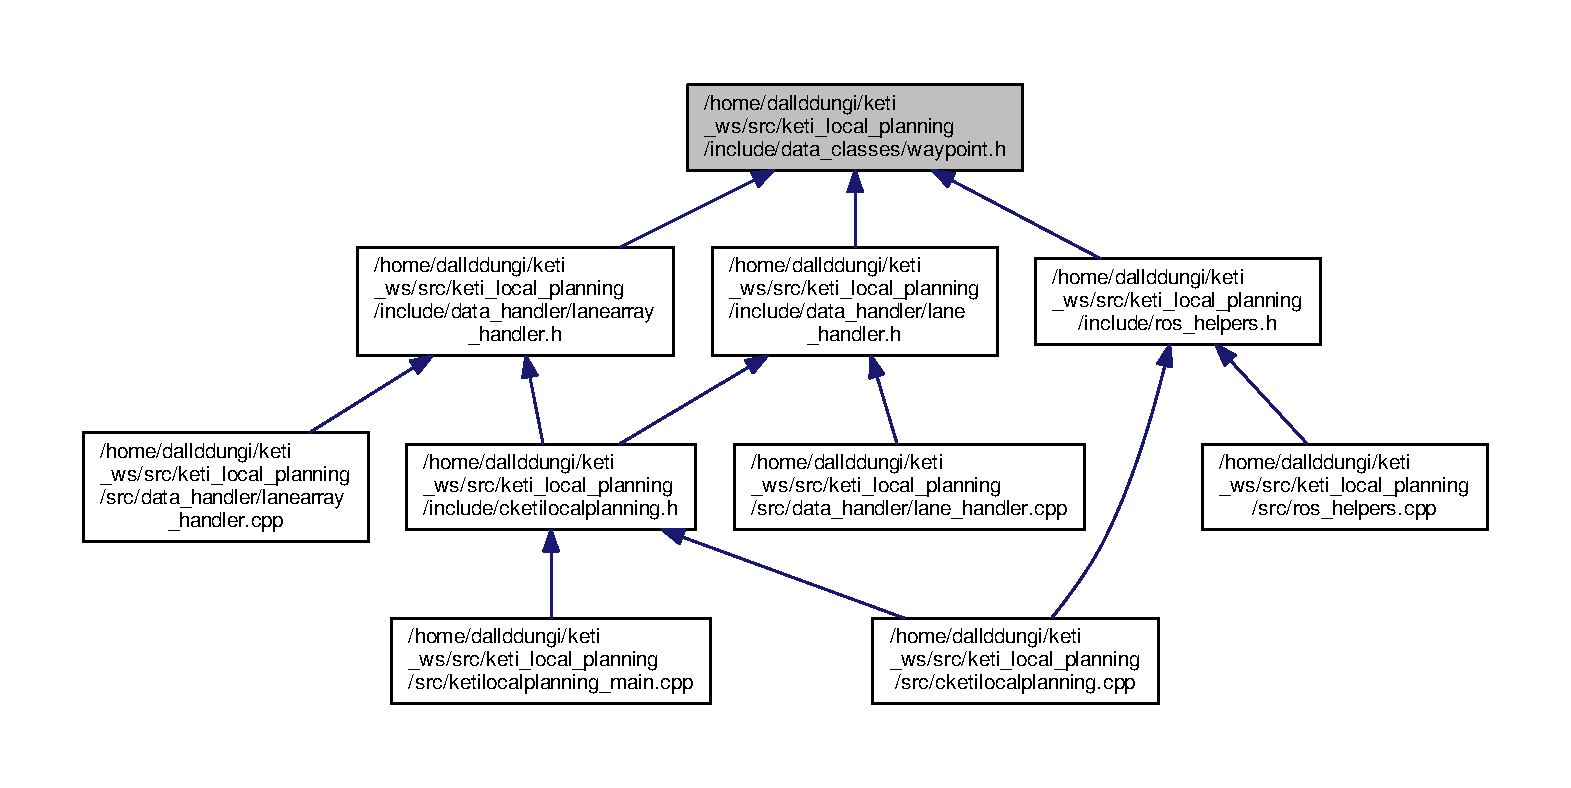
\includegraphics[width=350pt]{waypoint_8h__dep__incl}
\end{center}
\end{figure}
\subsection*{클래스}
\begin{DoxyCompactItemize}
\item 
class \hyperlink{class_way_point}{Way\+Point}
\begin{DoxyCompactList}\small\item\em type representing class containing (\hyperlink{class_g_p_s_point}{G\+P\+S\+Point}, v) \end{DoxyCompactList}\end{DoxyCompactItemize}

\hypertarget{lane__handler_8h}{}\section{/home/dallddungi/keti\+\_\+ws/src/keti\+\_\+local\+\_\+planning/include/data\+\_\+handler/lane\+\_\+handler.h 파일 참조}
\label{lane__handler_8h}\index{/home/dallddungi/keti\+\_\+ws/src/keti\+\_\+local\+\_\+planning/include/data\+\_\+handler/lane\+\_\+handler.\+h@{/home/dallddungi/keti\+\_\+ws/src/keti\+\_\+local\+\_\+planning/include/data\+\_\+handler/lane\+\_\+handler.\+h}}
{\ttfamily \#include \char`\"{}autoware\+\_\+msgs/lane.\+h\char`\"{}}\\*
{\ttfamily \#include \char`\"{}data\+\_\+classes/waypoint.\+h\char`\"{}}\\*
{\ttfamily \#include $<$geometry\+\_\+msgs/\+Point.\+h$>$}\\*
{\ttfamily \#include $<$geometry\+\_\+msgs/\+Pose.\+h$>$}\\*
lane\+\_\+handler.\+h에 대한 include 의존 그래프\nopagebreak
\begin{figure}[H]
\begin{center}
\leavevmode
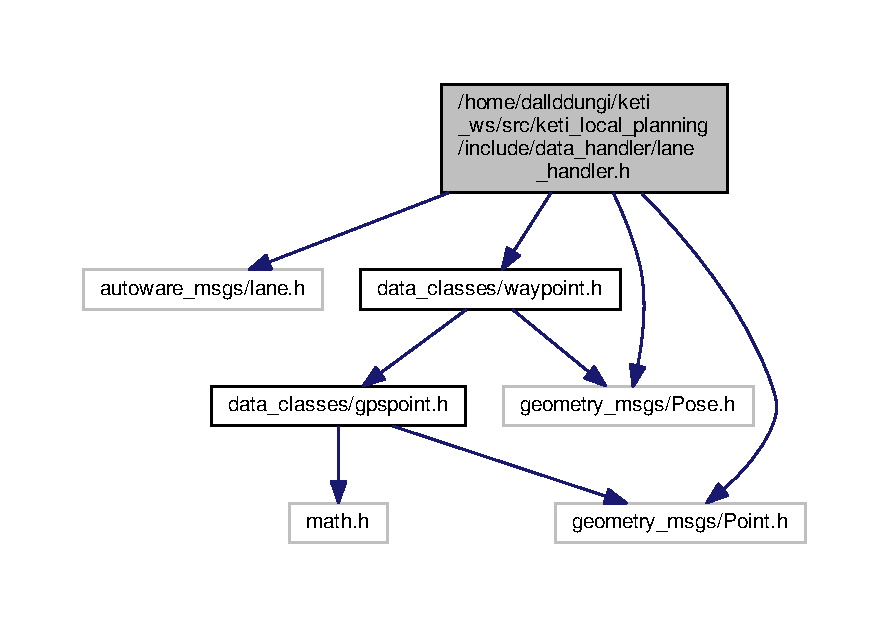
\includegraphics[width=350pt]{lane__handler_8h__incl}
\end{center}
\end{figure}
이 그래프는 이 파일을 직/간접적으로 include 하는 파일들을 보여줍니다.\+:\nopagebreak
\begin{figure}[H]
\begin{center}
\leavevmode
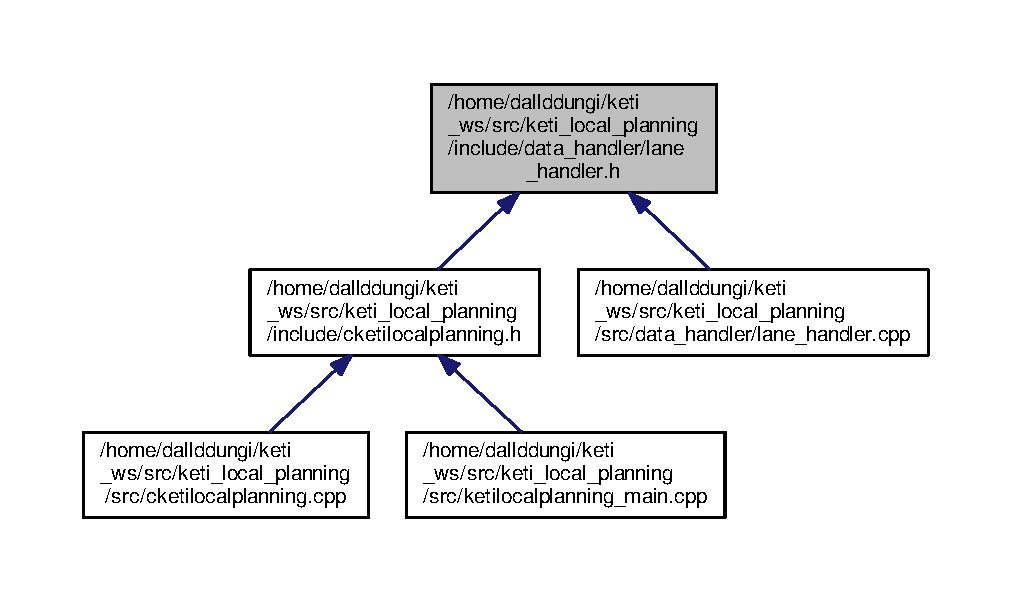
\includegraphics[width=350pt]{lane__handler_8h__dep__incl}
\end{center}
\end{figure}
\subsection*{클래스}
\begin{DoxyCompactItemize}
\item 
class \hyperlink{class_lane_handler}{Lane\+Handler}
\begin{DoxyCompactList}\small\item\em This class treats lane information with autowar\+\_\+msgs\+::lane and std\+::vector$<$\+Way\+Point$>$ \end{DoxyCompactList}\end{DoxyCompactItemize}

\hypertarget{lanearray__handler_8h}{}\section{/home/dallddungi/keti\+\_\+ws/src/keti\+\_\+local\+\_\+planning/include/data\+\_\+handler/lanearray\+\_\+handler.h 파일 참조}
\label{lanearray__handler_8h}\index{/home/dallddungi/keti\+\_\+ws/src/keti\+\_\+local\+\_\+planning/include/data\+\_\+handler/lanearray\+\_\+handler.\+h@{/home/dallddungi/keti\+\_\+ws/src/keti\+\_\+local\+\_\+planning/include/data\+\_\+handler/lanearray\+\_\+handler.\+h}}
{\ttfamily \#include \char`\"{}autoware\+\_\+msgs/\+Lane\+Array.\+h\char`\"{}}\\*
{\ttfamily \#include \char`\"{}autoware\+\_\+msgs/lane.\+h\char`\"{}}\\*
{\ttfamily \#include \char`\"{}data\+\_\+classes/waypoint.\+h\char`\"{}}\\*
lanearray\+\_\+handler.\+h에 대한 include 의존 그래프\nopagebreak
\begin{figure}[H]
\begin{center}
\leavevmode
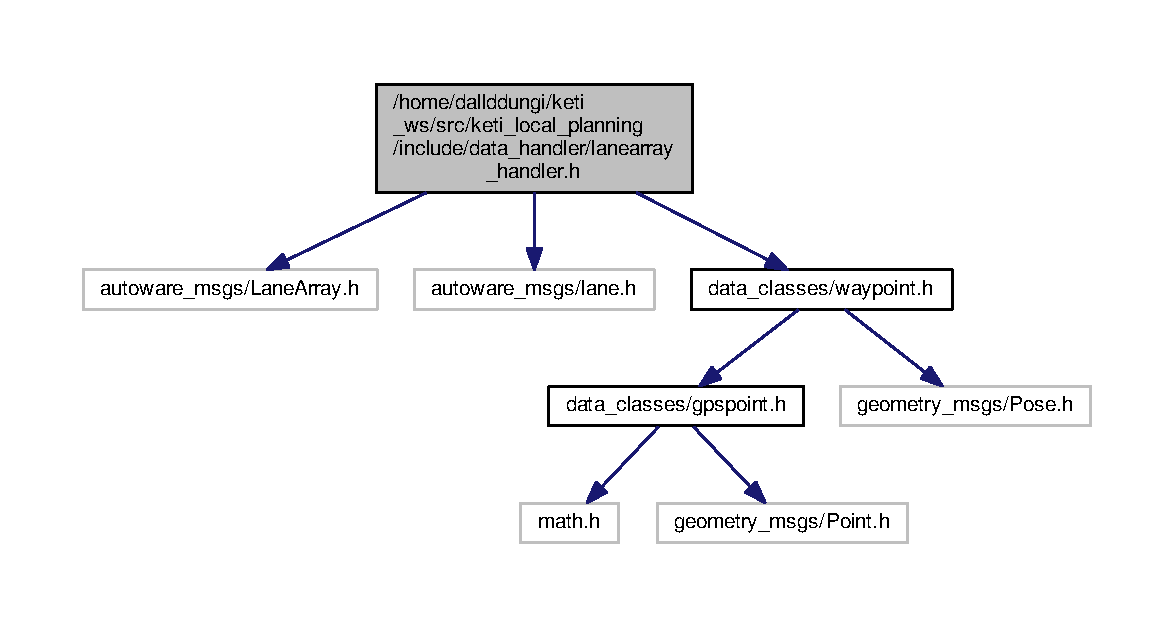
\includegraphics[width=350pt]{lanearray__handler_8h__incl}
\end{center}
\end{figure}
이 그래프는 이 파일을 직/간접적으로 include 하는 파일들을 보여줍니다.\+:\nopagebreak
\begin{figure}[H]
\begin{center}
\leavevmode
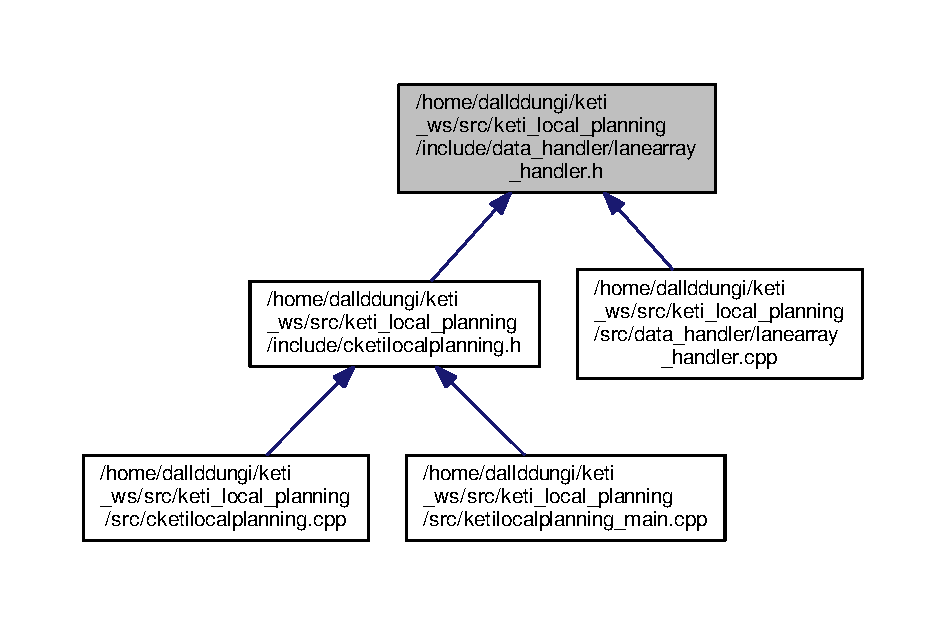
\includegraphics[width=350pt]{lanearray__handler_8h__dep__incl}
\end{center}
\end{figure}
\subsection*{클래스}
\begin{DoxyCompactItemize}
\item 
class \hyperlink{class_lane_array_handler}{Lane\+Array\+Handler}
\begin{DoxyCompactList}\small\item\em The Type\+Conversion class This class is handling lane array information. \end{DoxyCompactList}\end{DoxyCompactItemize}

\hypertarget{point__handler_8h}{}\section{/home/dallddungi/keti\+\_\+ws/src/keti\+\_\+local\+\_\+planning/include/data\+\_\+handler/point\+\_\+handler.h 파일 참조}
\label{point__handler_8h}\index{/home/dallddungi/keti\+\_\+ws/src/keti\+\_\+local\+\_\+planning/include/data\+\_\+handler/point\+\_\+handler.\+h@{/home/dallddungi/keti\+\_\+ws/src/keti\+\_\+local\+\_\+planning/include/data\+\_\+handler/point\+\_\+handler.\+h}}
{\ttfamily \#include $<$geometry\+\_\+msgs/\+Point.\+h$>$}\\*
point\+\_\+handler.\+h에 대한 include 의존 그래프\nopagebreak
\begin{figure}[H]
\begin{center}
\leavevmode
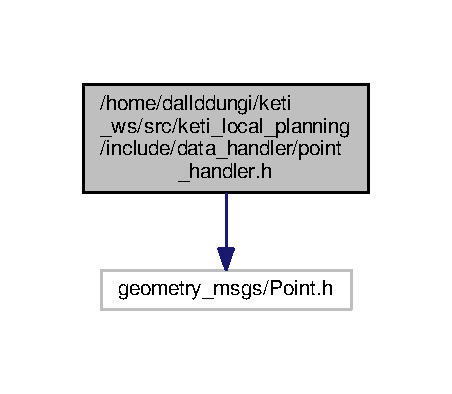
\includegraphics[width=217pt]{point__handler_8h__incl}
\end{center}
\end{figure}
\subsection*{클래스}
\begin{DoxyCompactItemize}
\item 
class \hyperlink{class_point_handler}{Point\+Handler}
\begin{DoxyCompactList}\small\item\em Point handling class. \end{DoxyCompactList}\item 
class \hyperlink{class_point_handler}{Point\+Handler}
\begin{DoxyCompactList}\small\item\em Point handling class. \end{DoxyCompactList}\end{DoxyCompactItemize}

\hypertarget{pose__point__handler_8h}{}\section{/home/dallddungi/keti\+\_\+ws/src/keti\+\_\+local\+\_\+planning/include/data\+\_\+handler/pose\+\_\+point\+\_\+handler.h 파일 참조}
\label{pose__point__handler_8h}\index{/home/dallddungi/keti\+\_\+ws/src/keti\+\_\+local\+\_\+planning/include/data\+\_\+handler/pose\+\_\+point\+\_\+handler.\+h@{/home/dallddungi/keti\+\_\+ws/src/keti\+\_\+local\+\_\+planning/include/data\+\_\+handler/pose\+\_\+point\+\_\+handler.\+h}}
{\ttfamily \#include $<$geometry\+\_\+msgs/\+Pose.\+h$>$}\\*
pose\+\_\+point\+\_\+handler.\+h에 대한 include 의존 그래프\nopagebreak
\begin{figure}[H]
\begin{center}
\leavevmode
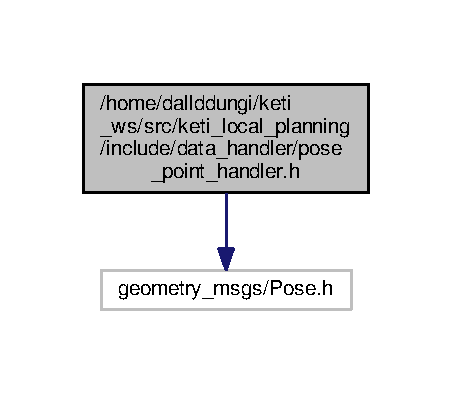
\includegraphics[width=217pt]{pose__point__handler_8h__incl}
\end{center}
\end{figure}
이 그래프는 이 파일을 직/간접적으로 include 하는 파일들을 보여줍니다.\+:\nopagebreak
\begin{figure}[H]
\begin{center}
\leavevmode
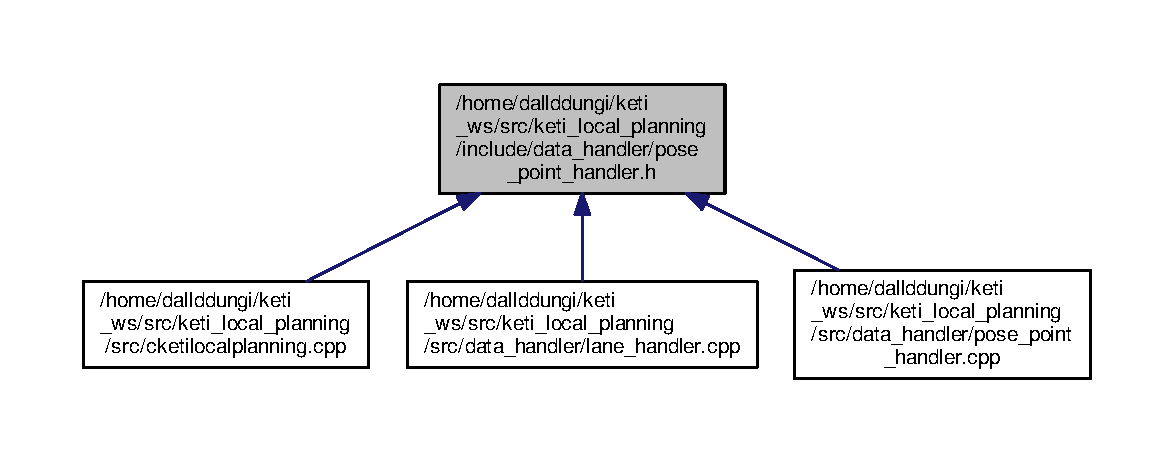
\includegraphics[width=350pt]{pose__point__handler_8h__dep__incl}
\end{center}
\end{figure}
\subsection*{클래스}
\begin{DoxyCompactItemize}
\item 
class \hyperlink{class_pose_point_handler}{Pose\+Point\+Handler}
\begin{DoxyCompactList}\small\item\em The Pose\+Position\+Handler class. \end{DoxyCompactList}\end{DoxyCompactItemize}

\hypertarget{projectinfo_8h}{}\section{/home/dallddungi/keti\+\_\+ws/src/keti\+\_\+local\+\_\+planning/include/projectinfo.h 파일 참조}
\label{projectinfo_8h}\index{/home/dallddungi/keti\+\_\+ws/src/keti\+\_\+local\+\_\+planning/include/projectinfo.\+h@{/home/dallddungi/keti\+\_\+ws/src/keti\+\_\+local\+\_\+planning/include/projectinfo.\+h}}

\hypertarget{ros__helpers_8h}{}\section{/home/dallddungi/keti\+\_\+ws/src/keti\+\_\+local\+\_\+planning/include/ros\+\_\+helpers.h 파일 참조}
\label{ros__helpers_8h}\index{/home/dallddungi/keti\+\_\+ws/src/keti\+\_\+local\+\_\+planning/include/ros\+\_\+helpers.\+h@{/home/dallddungi/keti\+\_\+ws/src/keti\+\_\+local\+\_\+planning/include/ros\+\_\+helpers.\+h}}
{\ttfamily \#include $<$visualization\+\_\+msgs/\+Marker\+Array.\+h$>$}\\*
{\ttfamily \#include \char`\"{}autoware\+\_\+msgs/lane.\+h\char`\"{}}\\*
{\ttfamily \#include $<$tf/tf.\+h$>$}\\*
{\ttfamily \#include \char`\"{}data\+\_\+classes/waypoint.\+h\char`\"{}}\\*
ros\+\_\+helpers.\+h에 대한 include 의존 그래프\nopagebreak
\begin{figure}[H]
\begin{center}
\leavevmode
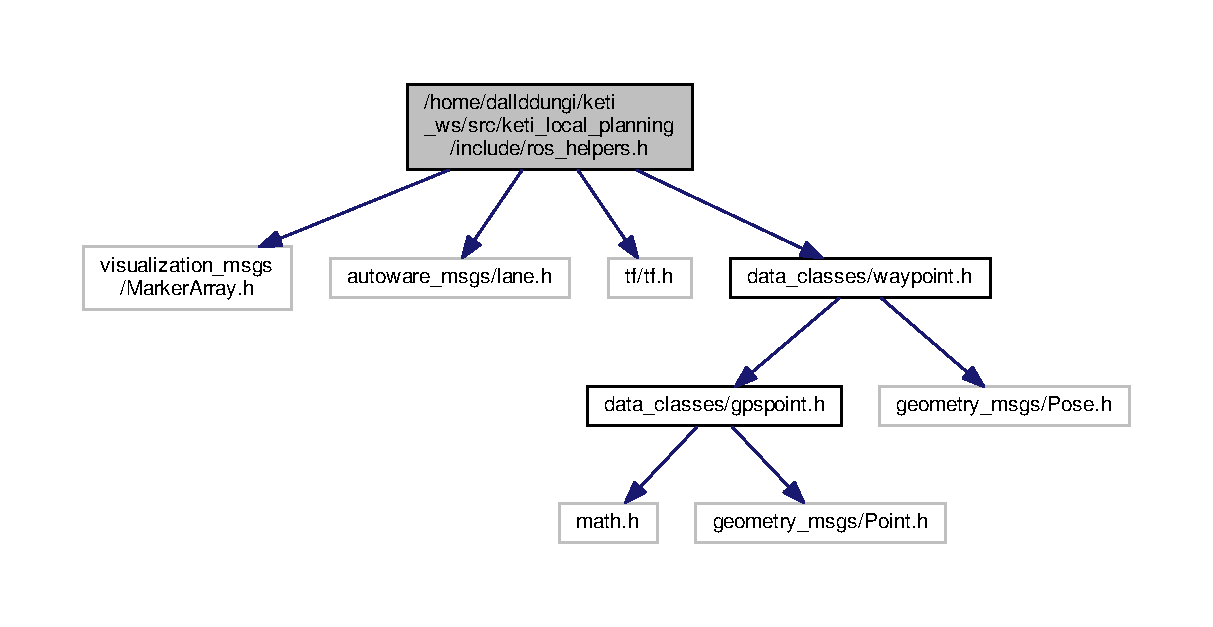
\includegraphics[width=350pt]{ros__helpers_8h__incl}
\end{center}
\end{figure}
이 그래프는 이 파일을 직/간접적으로 include 하는 파일들을 보여줍니다.\+:\nopagebreak
\begin{figure}[H]
\begin{center}
\leavevmode
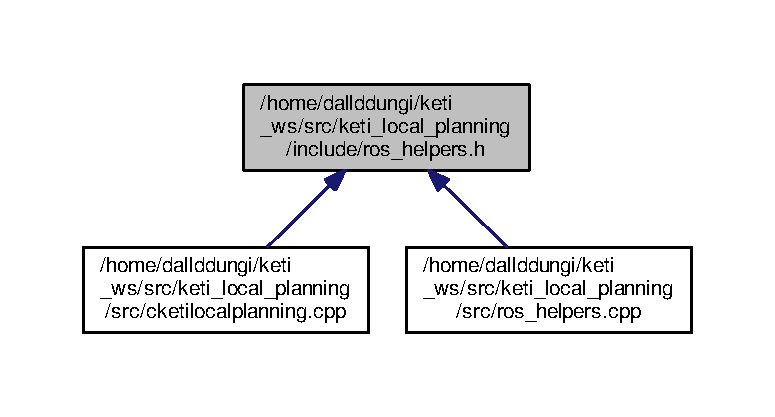
\includegraphics[width=350pt]{ros__helpers_8h__dep__incl}
\end{center}
\end{figure}
\subsection*{클래스}
\begin{DoxyCompactItemize}
\item 
class \hyperlink{class_ros_helpers}{Ros\+Helpers}
\end{DoxyCompactItemize}

\hypertarget{angle__utils_8h}{}\section{/home/dallddungi/keti\+\_\+ws/src/keti\+\_\+local\+\_\+planning/include/utils/angle\+\_\+utils.h 파일 참조}
\label{angle__utils_8h}\index{/home/dallddungi/keti\+\_\+ws/src/keti\+\_\+local\+\_\+planning/include/utils/angle\+\_\+utils.\+h@{/home/dallddungi/keti\+\_\+ws/src/keti\+\_\+local\+\_\+planning/include/utils/angle\+\_\+utils.\+h}}
{\ttfamily \#include $<$assert.\+h$>$}\\*
{\ttfamily \#include $<$string$>$}\\*
{\ttfamily \#include $<$math.\+h$>$}\\*
angle\+\_\+utils.\+h에 대한 include 의존 그래프\nopagebreak
\begin{figure}[H]
\begin{center}
\leavevmode
\includegraphics[width=257pt]{angle__utils_8h__incl}
\end{center}
\end{figure}
이 그래프는 이 파일을 직/간접적으로 include 하는 파일들을 보여줍니다.\+:\nopagebreak
\begin{figure}[H]
\begin{center}
\leavevmode
\includegraphics[width=350pt]{angle__utils_8h__dep__incl}
\end{center}
\end{figure}
\subsection*{클래스}
\begin{DoxyCompactItemize}
\item 
class \hyperlink{class_angle_utils}{Angle\+Utils}
\end{DoxyCompactItemize}

\hypertarget{math__constant_8h}{}\section{/home/dallddungi/keti\+\_\+ws/src/keti\+\_\+local\+\_\+planning/include/utils/math\+\_\+constant.h 파일 참조}
\label{math__constant_8h}\index{/home/dallddungi/keti\+\_\+ws/src/keti\+\_\+local\+\_\+planning/include/utils/math\+\_\+constant.\+h@{/home/dallddungi/keti\+\_\+ws/src/keti\+\_\+local\+\_\+planning/include/utils/math\+\_\+constant.\+h}}
{\ttfamily \#include $<$math.\+h$>$}\\*
math\+\_\+constant.\+h에 대한 include 의존 그래프\nopagebreak
\begin{figure}[H]
\begin{center}
\leavevmode
\includegraphics[width=227pt]{math__constant_8h__incl}
\end{center}
\end{figure}
\subsection*{함수}
\begin{DoxyCompactItemize}
\item 
{\footnotesize template$<$typename T $>$ }\\bool \hyperlink{math__constant_8h_a5e195fe2ba1896ebf32b3c92c0995315}{sign} (const T \&x)
\item 
{\footnotesize template$<$typename T $>$ }\\T \hyperlink{math__constant_8h_a83c0028e8e5f11951b04025d01ffe408}{min} (const T \&x, const T \&y)
\item 
{\footnotesize template$<$typename T $>$ }\\T \hyperlink{math__constant_8h_a0ddaec2f52f526234b051c9dff699a5f}{max} (const T \&x, const T \&y)
\end{DoxyCompactItemize}
\subsection*{변수}
\begin{DoxyCompactItemize}
\item 
const double \hyperlink{math__constant_8h_a3990c92eaf1a7084542e083950900d47}{D\+E\+G2\+R\+AD} = M\+\_\+\+PI / 180
\item 
const double \hyperlink{math__constant_8h_ada7628b7b7ccf0546436b9904cd76cd1}{R\+A\+D2\+D\+EG} = 180. / M\+\_\+\+PI
\end{DoxyCompactItemize}


\subsection{함수 문서화}
\index{math\+\_\+constant.\+h@{math\+\_\+constant.\+h}!max@{max}}
\index{max@{max}!math\+\_\+constant.\+h@{math\+\_\+constant.\+h}}
\subsubsection[{\texorpdfstring{max(const T \&x, const T \&y)}{max(const T &x, const T &y)}}]{\setlength{\rightskip}{0pt plus 5cm}template$<$typename T $>$ T max (
\begin{DoxyParamCaption}
\item[{const T \&}]{x, }
\item[{const T \&}]{y}
\end{DoxyParamCaption}
)\hspace{0.3cm}{\ttfamily [inline]}}\hypertarget{math__constant_8h_a0ddaec2f52f526234b051c9dff699a5f}{}\label{math__constant_8h_a0ddaec2f52f526234b051c9dff699a5f}


math\+\_\+constant.\+h 파일의 20 번째 라인에서 정의되었습니다.


\begin{DoxyCode}
21 \{
22   \textcolor{keywordflow}{return} (x >= y ? x : y);
23 \}
\end{DoxyCode}
\index{math\+\_\+constant.\+h@{math\+\_\+constant.\+h}!min@{min}}
\index{min@{min}!math\+\_\+constant.\+h@{math\+\_\+constant.\+h}}
\subsubsection[{\texorpdfstring{min(const T \&x, const T \&y)}{min(const T &x, const T &y)}}]{\setlength{\rightskip}{0pt plus 5cm}template$<$typename T $>$ T min (
\begin{DoxyParamCaption}
\item[{const T \&}]{x, }
\item[{const T \&}]{y}
\end{DoxyParamCaption}
)\hspace{0.3cm}{\ttfamily [inline]}}\hypertarget{math__constant_8h_a83c0028e8e5f11951b04025d01ffe408}{}\label{math__constant_8h_a83c0028e8e5f11951b04025d01ffe408}


math\+\_\+constant.\+h 파일의 14 번째 라인에서 정의되었습니다.


\begin{DoxyCode}
15 \{
16   \textcolor{keywordflow}{return} (x <= y ? x : y);
17 \}
\end{DoxyCode}
\index{math\+\_\+constant.\+h@{math\+\_\+constant.\+h}!sign@{sign}}
\index{sign@{sign}!math\+\_\+constant.\+h@{math\+\_\+constant.\+h}}
\subsubsection[{\texorpdfstring{sign(const T \&x)}{sign(const T &x)}}]{\setlength{\rightskip}{0pt plus 5cm}template$<$typename T $>$ bool sign (
\begin{DoxyParamCaption}
\item[{const T \&}]{x}
\end{DoxyParamCaption}
)\hspace{0.3cm}{\ttfamily [inline]}}\hypertarget{math__constant_8h_a5e195fe2ba1896ebf32b3c92c0995315}{}\label{math__constant_8h_a5e195fe2ba1896ebf32b3c92c0995315}


math\+\_\+constant.\+h 파일의 9 번째 라인에서 정의되었습니다.


\begin{DoxyCode}
9                             \{
10   \textcolor{keywordflow}{return} (x > 0) ? 1 : ((x < 0) ? -1 : 0);
11 \}
\end{DoxyCode}


\subsection{변수 문서화}
\index{math\+\_\+constant.\+h@{math\+\_\+constant.\+h}!D\+E\+G2\+R\+AD@{D\+E\+G2\+R\+AD}}
\index{D\+E\+G2\+R\+AD@{D\+E\+G2\+R\+AD}!math\+\_\+constant.\+h@{math\+\_\+constant.\+h}}
\subsubsection[{\texorpdfstring{D\+E\+G2\+R\+AD}{DEG2RAD}}]{\setlength{\rightskip}{0pt plus 5cm}const double D\+E\+G2\+R\+AD = M\+\_\+\+PI / 180}\hypertarget{math__constant_8h_a3990c92eaf1a7084542e083950900d47}{}\label{math__constant_8h_a3990c92eaf1a7084542e083950900d47}


math\+\_\+constant.\+h 파일의 5 번째 라인에서 정의되었습니다.

\index{math\+\_\+constant.\+h@{math\+\_\+constant.\+h}!R\+A\+D2\+D\+EG@{R\+A\+D2\+D\+EG}}
\index{R\+A\+D2\+D\+EG@{R\+A\+D2\+D\+EG}!math\+\_\+constant.\+h@{math\+\_\+constant.\+h}}
\subsubsection[{\texorpdfstring{R\+A\+D2\+D\+EG}{RAD2DEG}}]{\setlength{\rightskip}{0pt plus 5cm}const double R\+A\+D2\+D\+EG = 180. / M\+\_\+\+PI}\hypertarget{math__constant_8h_ada7628b7b7ccf0546436b9904cd76cd1}{}\label{math__constant_8h_ada7628b7b7ccf0546436b9904cd76cd1}


math\+\_\+constant.\+h 파일의 6 번째 라인에서 정의되었습니다.


\hypertarget{cketilocalplanning_8cpp}{}\section{/home/dallddungi/keti\+\_\+ws/src/keti\+\_\+local\+\_\+planning/src/cketilocalplanning.cpp 파일 참조}
\label{cketilocalplanning_8cpp}\index{/home/dallddungi/keti\+\_\+ws/src/keti\+\_\+local\+\_\+planning/src/cketilocalplanning.\+cpp@{/home/dallddungi/keti\+\_\+ws/src/keti\+\_\+local\+\_\+planning/src/cketilocalplanning.\+cpp}}
{\ttfamily \#include \char`\"{}cketilocalplanning.\+h\char`\"{}}\\*
{\ttfamily \#include $<$visualization\+\_\+msgs/\+Marker\+Array.\+h$>$}\\*
{\ttfamily \#include \char`\"{}data\+\_\+handler/pose\+\_\+point\+\_\+handler.\+h\char`\"{}}\\*
{\ttfamily \#include \char`\"{}ros\+\_\+helpers.\+h\char`\"{}}\\*
cketilocalplanning.\+cpp에 대한 include 의존 그래프\nopagebreak
\begin{figure}[H]
\begin{center}
\leavevmode
\includegraphics[width=350pt]{cketilocalplanning_8cpp__incl}
\end{center}
\end{figure}

\hypertarget{lane__handler_8cpp}{}\section{/home/dallddungi/keti\+\_\+ws/src/keti\+\_\+local\+\_\+planning/src/data\+\_\+handler/lane\+\_\+handler.cpp 파일 참조}
\label{lane__handler_8cpp}\index{/home/dallddungi/keti\+\_\+ws/src/keti\+\_\+local\+\_\+planning/src/data\+\_\+handler/lane\+\_\+handler.\+cpp@{/home/dallddungi/keti\+\_\+ws/src/keti\+\_\+local\+\_\+planning/src/data\+\_\+handler/lane\+\_\+handler.\+cpp}}
{\ttfamily \#include \char`\"{}data\+\_\+handler/lane\+\_\+handler.\+h\char`\"{}}\\*
{\ttfamily \#include $<$tf/tf.\+h$>$}\\*
{\ttfamily \#include \char`\"{}utils/angle\+\_\+utils.\+h\char`\"{}}\\*
{\ttfamily \#include \char`\"{}data\+\_\+handler/pose\+\_\+point\+\_\+handler.\+h\char`\"{}}\\*
lane\+\_\+handler.\+cpp에 대한 include 의존 그래프\nopagebreak
\begin{figure}[H]
\begin{center}
\leavevmode
\includegraphics[width=350pt]{lane__handler_8cpp__incl}
\end{center}
\end{figure}

\hypertarget{lanearray__handler_8cpp}{}\section{/home/dallddungi/keti\+\_\+ws/src/keti\+\_\+local\+\_\+planning/src/data\+\_\+handler/lanearray\+\_\+handler.cpp 파일 참조}
\label{lanearray__handler_8cpp}\index{/home/dallddungi/keti\+\_\+ws/src/keti\+\_\+local\+\_\+planning/src/data\+\_\+handler/lanearray\+\_\+handler.\+cpp@{/home/dallddungi/keti\+\_\+ws/src/keti\+\_\+local\+\_\+planning/src/data\+\_\+handler/lanearray\+\_\+handler.\+cpp}}
{\ttfamily \#include \char`\"{}data\+\_\+handler/lanearray\+\_\+handler.\+h\char`\"{}}\\*
{\ttfamily \#include $<$tf/tf.\+h$>$}\\*
lanearray\+\_\+handler.\+cpp에 대한 include 의존 그래프\nopagebreak
\begin{figure}[H]
\begin{center}
\leavevmode
\includegraphics[width=350pt]{lanearray__handler_8cpp__incl}
\end{center}
\end{figure}

\hypertarget{pose__point__handler_8cpp}{}\section{/home/dallddungi/keti\+\_\+ws/src/keti\+\_\+local\+\_\+planning/src/data\+\_\+handler/pose\+\_\+point\+\_\+handler.cpp 파일 참조}
\label{pose__point__handler_8cpp}\index{/home/dallddungi/keti\+\_\+ws/src/keti\+\_\+local\+\_\+planning/src/data\+\_\+handler/pose\+\_\+point\+\_\+handler.\+cpp@{/home/dallddungi/keti\+\_\+ws/src/keti\+\_\+local\+\_\+planning/src/data\+\_\+handler/pose\+\_\+point\+\_\+handler.\+cpp}}
{\ttfamily \#include \char`\"{}data\+\_\+handler/pose\+\_\+point\+\_\+handler.\+h\char`\"{}}\\*
{\ttfamily \#include \char`\"{}tf/tf.\+h\char`\"{}}\\*
pose\+\_\+point\+\_\+handler.\+cpp에 대한 include 의존 그래프\nopagebreak
\begin{figure}[H]
\begin{center}
\leavevmode
\includegraphics[width=261pt]{pose__point__handler_8cpp__incl}
\end{center}
\end{figure}

\hypertarget{ketilocalplanning__main_8cpp}{}\section{/home/dallddungi/keti\+\_\+ws/src/keti\+\_\+local\+\_\+planning/src/ketilocalplanning\+\_\+main.cpp 파일 참조}
\label{ketilocalplanning__main_8cpp}\index{/home/dallddungi/keti\+\_\+ws/src/keti\+\_\+local\+\_\+planning/src/ketilocalplanning\+\_\+main.\+cpp@{/home/dallddungi/keti\+\_\+ws/src/keti\+\_\+local\+\_\+planning/src/ketilocalplanning\+\_\+main.\+cpp}}
{\ttfamily \#include \char`\"{}cketilocalplanning.\+h\char`\"{}}\\*
{\ttfamily \#include $<$iostream$>$}\\*
ketilocalplanning\+\_\+main.\+cpp에 대한 include 의존 그래프\nopagebreak
\begin{figure}[H]
\begin{center}
\leavevmode
\includegraphics[width=350pt]{ketilocalplanning__main_8cpp__incl}
\end{center}
\end{figure}
\subsection*{함수}
\begin{DoxyCompactItemize}
\item 
int \hyperlink{ketilocalplanning__main_8cpp_a3c04138a5bfe5d72780bb7e82a18e627}{main} (int argc, char $\ast$$\ast$argv)
\end{DoxyCompactItemize}


\subsection{함수 문서화}
\index{ketilocalplanning\+\_\+main.\+cpp@{ketilocalplanning\+\_\+main.\+cpp}!main@{main}}
\index{main@{main}!ketilocalplanning\+\_\+main.\+cpp@{ketilocalplanning\+\_\+main.\+cpp}}
\subsubsection[{\texorpdfstring{main(int argc, char $\ast$$\ast$argv)}{main(int argc, char **argv)}}]{\setlength{\rightskip}{0pt plus 5cm}int main (
\begin{DoxyParamCaption}
\item[{int}]{argc, }
\item[{char $\ast$$\ast$}]{argv}
\end{DoxyParamCaption}
)}\hypertarget{ketilocalplanning__main_8cpp_a3c04138a5bfe5d72780bb7e82a18e627}{}\label{ketilocalplanning__main_8cpp_a3c04138a5bfe5d72780bb7e82a18e627}


ketilocalplanning\+\_\+main.\+cpp 파일의 7 번째 라인에서 정의되었습니다.


\begin{DoxyCode}
8 \{
9   ros::init(argc, argv, \textcolor{stringliteral}{"keti\_local\_planning"});
10   \hyperlink{class_c_keti_local_planning}{CKetiLocalPlanning} local\_planner;
11   local\_planner.\hyperlink{class_c_keti_local_planning_a3286318e734e7441036b43cec169978c}{PlannerMainLoop}();
12   \textcolor{keywordflow}{return} 0;
13 \}
\end{DoxyCode}


이 함수 내부에서 호출하는 함수들에 대한 그래프입니다.\+:\nopagebreak
\begin{figure}[H]
\begin{center}
\leavevmode
\includegraphics[width=350pt]{ketilocalplanning__main_8cpp_a3c04138a5bfe5d72780bb7e82a18e627_cgraph}
\end{center}
\end{figure}



\hypertarget{ros__helpers_8cpp}{}\section{/home/dallddungi/keti\+\_\+ws/src/keti\+\_\+local\+\_\+planning/src/ros\+\_\+helpers.cpp 파일 참조}
\label{ros__helpers_8cpp}\index{/home/dallddungi/keti\+\_\+ws/src/keti\+\_\+local\+\_\+planning/src/ros\+\_\+helpers.\+cpp@{/home/dallddungi/keti\+\_\+ws/src/keti\+\_\+local\+\_\+planning/src/ros\+\_\+helpers.\+cpp}}
{\ttfamily \#include \char`\"{}ros\+\_\+helpers.\+h\char`\"{}}\\*
ros\+\_\+helpers.\+cpp에 대한 include 의존 그래프\nopagebreak
\begin{figure}[H]
\begin{center}
\leavevmode
\includegraphics[width=350pt]{ros__helpers_8cpp__incl}
\end{center}
\end{figure}

\hypertarget{angle__utils_8cpp}{}\section{/home/dallddungi/keti\+\_\+ws/src/keti\+\_\+local\+\_\+planning/src/utils/angle\+\_\+utils.cpp 파일 참조}
\label{angle__utils_8cpp}\index{/home/dallddungi/keti\+\_\+ws/src/keti\+\_\+local\+\_\+planning/src/utils/angle\+\_\+utils.\+cpp@{/home/dallddungi/keti\+\_\+ws/src/keti\+\_\+local\+\_\+planning/src/utils/angle\+\_\+utils.\+cpp}}
{\ttfamily \#include \char`\"{}utils/angle\+\_\+utils.\+h\char`\"{}}\\*
angle\+\_\+utils.\+cpp에 대한 include 의존 그래프\nopagebreak
\begin{figure}[H]
\begin{center}
\leavevmode
\includegraphics[width=257pt]{angle__utils_8cpp__incl}
\end{center}
\end{figure}

%--- End generated contents ---

% Index
\backmatter
\newpage
\phantomsection
\clearemptydoublepage
\addcontentsline{toc}{chapter}{색인}
\printindex

\end{document}
